\documentclass[twoside]{book}

% Packages required by doxygen
\usepackage{fixltx2e}
\usepackage{calc}
\usepackage{doxygen}
\usepackage[export]{adjustbox} % also loads graphicx
\usepackage{graphicx}
\usepackage[utf8]{inputenc}
\usepackage{makeidx}
\usepackage{multicol}
\usepackage{multirow}
\PassOptionsToPackage{warn}{textcomp}
\usepackage{textcomp}
\usepackage[nointegrals]{wasysym}
\usepackage[table]{xcolor}

% Font selection
\usepackage[T1]{fontenc}
\usepackage[scaled=.90]{helvet}
\usepackage{courier}
\usepackage{amssymb}
\usepackage{sectsty}
\renewcommand{\familydefault}{\sfdefault}
\allsectionsfont{%
  \fontseries{bc}\selectfont%
  \color{darkgray}%
}
\renewcommand{\DoxyLabelFont}{%
  \fontseries{bc}\selectfont%
  \color{darkgray}%
}
\newcommand{\+}{\discretionary{\mbox{\scriptsize$\hookleftarrow$}}{}{}}

% Page & text layout
\usepackage{geometry}
\geometry{%
  a4paper,%
  top=2.5cm,%
  bottom=2.5cm,%
  left=2.5cm,%
  right=2.5cm%
}
\tolerance=750
\hfuzz=15pt
\hbadness=750
\setlength{\emergencystretch}{15pt}
\setlength{\parindent}{0cm}
\setlength{\parskip}{3ex plus 2ex minus 2ex}
\makeatletter
\renewcommand{\paragraph}{%
  \@startsection{paragraph}{4}{0ex}{-1.0ex}{1.0ex}{%
    \normalfont\normalsize\bfseries\SS@parafont%
  }%
}
\renewcommand{\subparagraph}{%
  \@startsection{subparagraph}{5}{0ex}{-1.0ex}{1.0ex}{%
    \normalfont\normalsize\bfseries\SS@subparafont%
  }%
}
\makeatother

% Headers & footers
\usepackage{fancyhdr}
\pagestyle{fancyplain}
\fancyhead[LE]{\fancyplain{}{\bfseries\thepage}}
\fancyhead[CE]{\fancyplain{}{}}
\fancyhead[RE]{\fancyplain{}{\bfseries\leftmark}}
\fancyhead[LO]{\fancyplain{}{\bfseries\rightmark}}
\fancyhead[CO]{\fancyplain{}{}}
\fancyhead[RO]{\fancyplain{}{\bfseries\thepage}}
\fancyfoot[LE]{\fancyplain{}{}}
\fancyfoot[CE]{\fancyplain{}{}}
\fancyfoot[RE]{\fancyplain{}{\bfseries\scriptsize 構築\+: Doxygen }}
\fancyfoot[LO]{\fancyplain{}{\bfseries\scriptsize 構築\+: Doxygen }}
\fancyfoot[CO]{\fancyplain{}{}}
\fancyfoot[RO]{\fancyplain{}{}}
\renewcommand{\footrulewidth}{0.4pt}
\renewcommand{\chaptermark}[1]{%
  \markboth{#1}{}%
}
\renewcommand{\sectionmark}[1]{%
  \markright{\thesection\ #1}%
}

% Indices & bibliography
\usepackage{natbib}
\usepackage[titles]{tocloft}
\setcounter{tocdepth}{3}
\setcounter{secnumdepth}{5}
\makeindex

% Hyperlinks (required, but should be loaded last)
\usepackage{ifpdf}
\ifpdf
  \usepackage[pdftex,pagebackref=true]{hyperref}
\else
  \usepackage[ps2pdf,pagebackref=true]{hyperref}
\fi
\hypersetup{%
  colorlinks=true,%
  linkcolor=blue,%
  citecolor=blue,%
  unicode%
}

% Custom commands
\newcommand{\clearemptydoublepage}{%
  \newpage{\pagestyle{empty}\cleardoublepage}%
}

\usepackage{caption}
\captionsetup{labelsep=space,justification=centering,font={bf},singlelinecheck=off,skip=4pt,position=top}

%===== C O N T E N T S =====

\begin{document}

% Titlepage & ToC
\hypersetup{pageanchor=false,
             bookmarksnumbered=true,
             pdfencoding=unicode
            }
\pagenumbering{alph}
\begin{titlepage}
\vspace*{7cm}
\begin{center}%
{\Large M\+C\+MS }\\
\vspace*{1cm}
{\large 構築\+: Doxygen 1.8.13}\\
\end{center}
\end{titlepage}
\clearemptydoublepage
\pagenumbering{roman}
\tableofcontents
\clearemptydoublepage
\pagenumbering{arabic}
\hypersetup{pageanchor=true}

%--- Begin generated contents ---
\chapter{todo一覧}
\label{todo}
\Hypertarget{todo}

\begin{DoxyRefList}
\item[\label{todo__todo000002}%
\Hypertarget{todo__todo000002}%
メンバ \hyperlink{class_t_k_a_d_c_c_o_n_t_r_o_l_afa385509f61162198950676d279f4c3c}{T\+K\+A\+D\+C\+C\+O\+N\+T\+R\+OL\+:\+:Delete} (std\+::string file\+\_\+name)]許されないファイル名を拒否する  
\item[\label{todo__todo000003}%
\Hypertarget{todo__todo000003}%
メンバ \hyperlink{class_t_k_a_d_c_c_o_n_t_r_o_l_afbeba1999b1d5afeda2d3b755d20b2ce}{T\+K\+A\+D\+C\+C\+O\+N\+T\+R\+OL\+:\+:Get\+Last\+Local\+Shot\+Number} ()]A\+D\+Cコントロールクラスに存在するのは不適当なので別のクラスに移動させる  
\item[\label{todo__todo000001}%
\Hypertarget{todo__todo000001}%
メンバ \hyperlink{class_t_k_a_d_c_c_o_n_t_r_o_l_a832915af5a7240efeef5c3fa139b99af}{T\+K\+A\+D\+C\+C\+O\+N\+T\+R\+OL\+:\+:Save\+Shot} (std\+::string file\+\_\+name)]保存されたファイル名の取得 

許されないファイル名を拒否する  
\item[\label{todo__todo000004}%
\Hypertarget{todo__todo000004}%
メンバ \hyperlink{class_t_k_a_n_a_l_y_z_e_ae7ea90bd92b92e5e75f89a5c5c6bbabb}{T\+K\+A\+N\+A\+L\+Y\+ZE\+:\+:calc\+Surface\+Area} (T\+K\+Charged\+Particle\+Type particle\+\_\+type)]計算手法を\+P\+R\+E\+D\+A\+T\+A\+P\+R\+O\+C\+E\+S\+S同様enum化する。~\newline
 引数が不適切であるので廃止してラッパ関数を用意する。 
\end{DoxyRefList}
\chapter{名前空間索引}
\section{名前空間一覧}
詳解が付いた名前空間の一覧です。\begin{DoxyCompactList}
\item\contentsline{section}{\hyperlink{namespace_t_k_f_i_l_e_u_t_i_l}{T\+K\+F\+I\+L\+E\+U\+T\+IL} \\*便利な汎用関数等です。 }{\pageref{namespace_t_k_f_i_l_e_u_t_i_l}}{}
\item\contentsline{section}{\hyperlink{namespace_t_k_u_t_i_l}{T\+K\+U\+T\+IL} \\*便利な汎用関数等です。 }{\pageref{namespace_t_k_u_t_i_l}}{}
\item\contentsline{section}{\hyperlink{namespace_t_k_u_t_i_l_1_1_literals}{T\+K\+U\+T\+I\+L\+::\+Literals} }{\pageref{namespace_t_k_u_t_i_l_1_1_literals}}{}
\end{DoxyCompactList}

\chapter{階層索引}
\section{クラス階層}
クラス階層一覧です。大雑把に文字符号順で並べられています。\begin{DoxyCompactList}
\item \contentsline{section}{\+\_\+\+Devicelist}{\pageref{struct___devicelist}}{}
\item \contentsline{section}{\+\_\+\+Devicelist\+Ex}{\pageref{struct___devicelist_ex}}{}
\item bad\+\_\+cast\begin{DoxyCompactList}
\item \contentsline{section}{Project1\+:\+:My\+Form\+:\+:clx\+:\+:bad\+\_\+lexical\+\_\+cast}{\pageref{class_project1_1_1_my_form_1_1clx_1_1bad__lexical__cast}}{}
\end{DoxyCompactList}
\item \contentsline{section}{Project1\+:\+:My\+Form\+:\+:clx\+:\+:cast\+\_\+stream$<$ Type, Source $>$}{\pageref{class_project1_1_1_my_form_1_1clx_1_1cast__stream}}{}
\item \contentsline{section}{Project1\+:\+:My\+Form\+:\+:clx\+:\+:charset\+\_\+functor$<$ CharT $>$}{\pageref{class_project1_1_1_my_form_1_1clx_1_1charset__functor}}{}
\item \contentsline{section}{Project1\+:\+:My\+Form\+:\+:clx\+:\+:classified\+\_\+functor}{\pageref{class_project1_1_1_my_form_1_1clx_1_1classified__functor}}{}
\item \contentsline{section}{D\+E\+V\+I\+CE}{\pageref{struct_d_e_v_i_c_e}}{}
\item \contentsline{section}{exadcstart}{\pageref{classexadcstart}}{}
\item \contentsline{section}{exfunctor}{\pageref{classexfunctor}}{}
\item Form\begin{DoxyCompactList}
\item \contentsline{section}{Project1\+:\+:My\+Form}{\pageref{class_project1_1_1_my_form}}{}
\item \contentsline{section}{Project1\+:\+:Setup\+A\+D\+C\+Connection}{\pageref{class_project1_1_1_setup_a_d_c_connection}}{}
\item \contentsline{section}{Project1\+:\+:Setup\+A\+D\+C\+Measurement}{\pageref{class_project1_1_1_setup_a_d_c_measurement}}{}
\item \contentsline{section}{Project1\+:\+:Setup\+Analyze\+SP}{\pageref{class_project1_1_1_setup_analyze_s_p}}{}
\item \contentsline{section}{Project1\+:\+:Setup\+Plot}{\pageref{class_project1_1_1_setup_plot}}{}
\end{DoxyCompactList}
\item \contentsline{section}{T\+K\+P\+L\+OT\+:\+:P\+L\+O\+T\+I\+N\+FO}{\pageref{struct_t_k_p_l_o_t_1_1_p_l_o_t_i_n_f_o}}{}
\item \contentsline{section}{T\+K\+P\+L\+OT\+:\+:P\+O\+S\+I\+T\+I\+ON$<$ T $>$}{\pageref{class_t_k_p_l_o_t_1_1_p_o_s_i_t_i_o_n}}{}
\item \contentsline{section}{T\+K\+P\+L\+OT\+:\+:P\+O\+S\+I\+T\+I\+ON$<$ int $>$}{\pageref{class_t_k_p_l_o_t_1_1_p_o_s_i_t_i_o_n}}{}
\item \contentsline{section}{T\+K\+P\+L\+OT\+:\+:R\+A\+N\+GE$<$ T $>$}{\pageref{class_t_k_p_l_o_t_1_1_r_a_n_g_e}}{}
\item \contentsline{section}{T\+K\+P\+L\+OT\+:\+:R\+A\+N\+GE$<$ float $>$}{\pageref{class_t_k_p_l_o_t_1_1_r_a_n_g_e}}{}
\item \contentsline{section}{T\+K\+P\+L\+OT\+:\+:S\+I\+ZE$<$ T $>$}{\pageref{class_t_k_p_l_o_t_1_1_s_i_z_e}}{}
\item \contentsline{section}{T\+K\+P\+L\+OT\+:\+:S\+I\+ZE$<$ int $>$}{\pageref{class_t_k_p_l_o_t_1_1_s_i_z_e}}{}
\item \contentsline{section}{Project1\+:\+:My\+Form\+:\+:clx\+:\+:detail\+:\+:stream\+\_\+char$<$ Type $>$}{\pageref{struct_project1_1_1_my_form_1_1clx_1_1detail_1_1stream__char}}{}
\item \contentsline{section}{T\+K\+A\+DC}{\pageref{class_t_k_a_d_c}}{}
\begin{DoxyCompactList}
\item \contentsline{section}{T\+K\+A\+D\+C\+\_\+\+D\+L750}{\pageref{class_t_k_a_d_c___d_l750}}{}
\item \contentsline{section}{T\+K\+A\+D\+C\+\_\+\+D\+L850}{\pageref{class_t_k_a_d_c___d_l850}}{}
\end{DoxyCompactList}
\item \contentsline{section}{T\+K\+A\+N\+A\+L\+Y\+Z\+E\+SP}{\pageref{class_t_k_a_n_a_l_y_z_e_s_p}}{}
\item \contentsline{section}{T\+K\+D\+A\+TA}{\pageref{class_t_k_d_a_t_a}}{}
\item \contentsline{section}{T\+K\+Particle\+Palameter}{\pageref{class_t_k_particle_palameter}}{}
\item \contentsline{section}{T\+K\+Plasma}{\pageref{class_t_k_plasma}}{}
\item \contentsline{section}{T\+K\+Plasma\+Parameter}{\pageref{class_t_k_plasma_parameter}}{}
\item \contentsline{section}{T\+K\+P\+L\+OT}{\pageref{class_t_k_p_l_o_t}}{}
\item \contentsline{section}{T\+K\+S\+H\+OT}{\pageref{class_t_k_s_h_o_t}}{}
\item \contentsline{section}{Project1\+:\+:My\+Form\+:\+:clx\+:\+:detail\+:\+:widest\+\_\+char$<$ Type\+Char, Source\+Char $>$}{\pageref{struct_project1_1_1_my_form_1_1clx_1_1detail_1_1widest__char}}{}
\end{DoxyCompactList}

\chapter{クラス索引}
\section{クラス一覧}
クラス・構造体・共用体・インターフェースの一覧です。\begin{DoxyCompactList}
\item\contentsline{section}{\hyperlink{struct___devicelist}{\+\_\+\+Devicelist} }{\pageref{struct___devicelist}}{}
\item\contentsline{section}{\hyperlink{struct___devicelist_ex}{\+\_\+\+Devicelist\+Ex} }{\pageref{struct___devicelist_ex}}{}
\item\contentsline{section}{\hyperlink{class_project1_1_1_dialog_quick_load_shot}{Project1\+::\+Dialog\+Quick\+Load\+Shot} \\*\hyperlink{class_project1_1_1_dialog_quick_load_shot}{Dialog\+Quick\+Load\+Shot} の概要 }{\pageref{class_project1_1_1_dialog_quick_load_shot}}{}
\item\contentsline{section}{\hyperlink{classtinyxml2_1_1_dyn_array}{tinyxml2\+::\+Dyn\+Array$<$ T, I\+N\+I\+T\+I\+A\+L\+\_\+\+S\+I\+Z\+E $>$} }{\pageref{classtinyxml2_1_1_dyn_array}}{}
\item\contentsline{section}{\hyperlink{structtinyxml2_1_1_entity}{tinyxml2\+::\+Entity} }{\pageref{structtinyxml2_1_1_entity}}{}
\item\contentsline{section}{\hyperlink{classexadcstart}{exadcstart} }{\pageref{classexadcstart}}{}
\item\contentsline{section}{\hyperlink{class_t_k_a_d_c_c_o_n_t_r_o_l_1_1_exception}{T\+K\+A\+D\+C\+C\+O\+N\+T\+R\+O\+L\+::\+Exception} }{\pageref{class_t_k_a_d_c_c_o_n_t_r_o_l_1_1_exception}}{}
\item\contentsline{section}{\hyperlink{classexfunctor}{exfunctor} }{\pageref{classexfunctor}}{}
\item\contentsline{section}{\hyperlink{class_t_k_a_n_a_l_y_z_e_1_1_f_i_t_r_a_n_g_e}{T\+K\+A\+N\+A\+L\+Y\+Z\+E\+::\+F\+I\+T\+R\+A\+N\+GE} }{\pageref{class_t_k_a_n_a_l_y_z_e_1_1_f_i_t_r_a_n_g_e}}{}
\item\contentsline{section}{\hyperlink{structtinyxml2_1_1_long_fits_into_size_t_minus_one}{tinyxml2\+::\+Long\+Fits\+Into\+Size\+T\+Minus\+One$<$ bool $>$} }{\pageref{structtinyxml2_1_1_long_fits_into_size_t_minus_one}}{}
\item\contentsline{section}{\hyperlink{structtinyxml2_1_1_long_fits_into_size_t_minus_one_3_01false_01_4}{tinyxml2\+::\+Long\+Fits\+Into\+Size\+T\+Minus\+One$<$ false $>$} }{\pageref{structtinyxml2_1_1_long_fits_into_size_t_minus_one_3_01false_01_4}}{}
\item\contentsline{section}{\hyperlink{classtinyxml2_1_1_mem_pool}{tinyxml2\+::\+Mem\+Pool} }{\pageref{classtinyxml2_1_1_mem_pool}}{}
\item\contentsline{section}{\hyperlink{classtinyxml2_1_1_mem_pool_t}{tinyxml2\+::\+Mem\+Pool\+T$<$ I\+T\+E\+M\+\_\+\+S\+I\+Z\+E $>$} }{\pageref{classtinyxml2_1_1_mem_pool_t}}{}
\item\contentsline{section}{\hyperlink{class_project1_1_1_my_form}{Project1\+::\+My\+Form} \\*\hyperlink{class_project1_1_1_my_form}{My\+Form} の概要 }{\pageref{class_project1_1_1_my_form}}{}
\item\contentsline{section}{\hyperlink{class_project1_1_1_setup_a_d_c_connection}{Project1\+::\+Setup\+A\+D\+C\+Connection} \\*\hyperlink{class_project1_1_1_setup_a_d_c_connection}{Setup\+A\+D\+C\+Connection} の概要 }{\pageref{class_project1_1_1_setup_a_d_c_connection}}{}
\item\contentsline{section}{\hyperlink{class_project1_1_1_setup_a_d_c_measurement}{Project1\+::\+Setup\+A\+D\+C\+Measurement} \\*\hyperlink{class_project1_1_1_setup_a_d_c_measurement}{Setup\+A\+D\+C\+Measurement} の概要 }{\pageref{class_project1_1_1_setup_a_d_c_measurement}}{}
\item\contentsline{section}{\hyperlink{class_project1_1_1_setup_analyze_s_p}{Project1\+::\+Setup\+Analyze\+SP} \\*\hyperlink{class_project1_1_1_setup_analyze_s_p}{Setup\+Analyze\+SP} の概要 }{\pageref{class_project1_1_1_setup_analyze_s_p}}{}
\item\contentsline{section}{\hyperlink{class_project1_1_1_setup_plot}{Project1\+::\+Setup\+Plot} \\*\hyperlink{class_project1_1_1_setup_plot}{Setup\+Plot} の概要 }{\pageref{class_project1_1_1_setup_plot}}{}
\item\contentsline{section}{\hyperlink{class_t_k_f_i_l_e_u_t_i_l_1_1_s_h_o_t_f_i_l_e_n_a_m_e}{T\+K\+F\+I\+L\+E\+U\+T\+I\+L\+::\+S\+H\+O\+T\+F\+I\+L\+E\+N\+A\+ME} }{\pageref{class_t_k_f_i_l_e_u_t_i_l_1_1_s_h_o_t_f_i_l_e_n_a_m_e}}{}
\item\contentsline{section}{\hyperlink{classtinyxml2_1_1_str_pair}{tinyxml2\+::\+Str\+Pair} }{\pageref{classtinyxml2_1_1_str_pair}}{}
\item\contentsline{section}{\hyperlink{class_t_k_a_d_c_c_o_n_t_r_o_l}{T\+K\+A\+D\+C\+C\+O\+N\+T\+R\+OL} }{\pageref{class_t_k_a_d_c_c_o_n_t_r_o_l}}{}
\item\contentsline{section}{\hyperlink{class_t_k_a_d_c_c_o_n_t_r_o_l___d_l750}{T\+K\+A\+D\+C\+C\+O\+N\+T\+R\+O\+L\+\_\+\+D\+L750} }{\pageref{class_t_k_a_d_c_c_o_n_t_r_o_l___d_l750}}{}
\item\contentsline{section}{\hyperlink{class_t_k_a_d_c_c_o_n_t_r_o_l___d_l850}{T\+K\+A\+D\+C\+C\+O\+N\+T\+R\+O\+L\+\_\+\+D\+L850} }{\pageref{class_t_k_a_d_c_c_o_n_t_r_o_l___d_l850}}{}
\item\contentsline{section}{\hyperlink{class_t_k_a_n_a_l_y_z_e}{T\+K\+A\+N\+A\+L\+Y\+ZE} }{\pageref{class_t_k_a_n_a_l_y_z_e}}{}
\item\contentsline{section}{\hyperlink{class_t_k_d_a_t_a}{T\+K\+D\+A\+TA} }{\pageref{class_t_k_d_a_t_a}}{}
\item\contentsline{section}{\hyperlink{class_t_k_particle_palameter}{T\+K\+Particle\+Palameter} }{\pageref{class_t_k_particle_palameter}}{}
\item\contentsline{section}{\hyperlink{class_t_k_plasma}{T\+K\+Plasma} }{\pageref{class_t_k_plasma}}{}
\item\contentsline{section}{\hyperlink{class_t_k_plasma_parameter}{T\+K\+Plasma\+Parameter} }{\pageref{class_t_k_plasma_parameter}}{}
\item\contentsline{section}{\hyperlink{class_t_k_s_h_o_t}{T\+K\+S\+H\+OT} }{\pageref{class_t_k_s_h_o_t}}{}
\item\contentsline{section}{\hyperlink{classtinyxml2_1_1_x_m_l_attribute}{tinyxml2\+::\+X\+M\+L\+Attribute} }{\pageref{classtinyxml2_1_1_x_m_l_attribute}}{}
\item\contentsline{section}{\hyperlink{classtinyxml2_1_1_x_m_l_comment}{tinyxml2\+::\+X\+M\+L\+Comment} }{\pageref{classtinyxml2_1_1_x_m_l_comment}}{}
\item\contentsline{section}{\hyperlink{classtinyxml2_1_1_x_m_l_const_handle}{tinyxml2\+::\+X\+M\+L\+Const\+Handle} }{\pageref{classtinyxml2_1_1_x_m_l_const_handle}}{}
\item\contentsline{section}{\hyperlink{classtinyxml2_1_1_x_m_l_declaration}{tinyxml2\+::\+X\+M\+L\+Declaration} }{\pageref{classtinyxml2_1_1_x_m_l_declaration}}{}
\item\contentsline{section}{\hyperlink{classtinyxml2_1_1_x_m_l_document}{tinyxml2\+::\+X\+M\+L\+Document} }{\pageref{classtinyxml2_1_1_x_m_l_document}}{}
\item\contentsline{section}{\hyperlink{classtinyxml2_1_1_x_m_l_element}{tinyxml2\+::\+X\+M\+L\+Element} }{\pageref{classtinyxml2_1_1_x_m_l_element}}{}
\item\contentsline{section}{\hyperlink{classtinyxml2_1_1_x_m_l_handle}{tinyxml2\+::\+X\+M\+L\+Handle} }{\pageref{classtinyxml2_1_1_x_m_l_handle}}{}
\item\contentsline{section}{\hyperlink{classtinyxml2_1_1_x_m_l_node}{tinyxml2\+::\+X\+M\+L\+Node} }{\pageref{classtinyxml2_1_1_x_m_l_node}}{}
\item\contentsline{section}{\hyperlink{classtinyxml2_1_1_x_m_l_printer}{tinyxml2\+::\+X\+M\+L\+Printer} }{\pageref{classtinyxml2_1_1_x_m_l_printer}}{}
\item\contentsline{section}{\hyperlink{classtinyxml2_1_1_x_m_l_text}{tinyxml2\+::\+X\+M\+L\+Text} }{\pageref{classtinyxml2_1_1_x_m_l_text}}{}
\item\contentsline{section}{\hyperlink{classtinyxml2_1_1_x_m_l_unknown}{tinyxml2\+::\+X\+M\+L\+Unknown} }{\pageref{classtinyxml2_1_1_x_m_l_unknown}}{}
\item\contentsline{section}{\hyperlink{classtinyxml2_1_1_x_m_l_util}{tinyxml2\+::\+X\+M\+L\+Util} }{\pageref{classtinyxml2_1_1_x_m_l_util}}{}
\item\contentsline{section}{\hyperlink{classtinyxml2_1_1_x_m_l_visitor}{tinyxml2\+::\+X\+M\+L\+Visitor} }{\pageref{classtinyxml2_1_1_x_m_l_visitor}}{}
\end{DoxyCompactList}

\chapter{ファイル索引}
\section{ファイル一覧}
詳解が付けられているファイルの一覧です。\begin{DoxyCompactList}
\item\contentsline{section}{U\+I/\+Project1/{\bfseries My\+Form.\+h} }{\pageref{_my_form_8h}}{}
\item\contentsline{section}{U\+I/\+Project1/{\bfseries resource.\+h} }{\pageref{resource_8h}}{}
\item\contentsline{section}{U\+I/\+Project1/{\bfseries resource1.\+h} }{\pageref{resource1_8h}}{}
\item\contentsline{section}{U\+I/\+Project1/{\bfseries Setup\+A\+D\+C\+Connection.\+h} }{\pageref{_setup_a_d_c_connection_8h}}{}
\item\contentsline{section}{U\+I/\+Project1/{\bfseries Setup\+A\+D\+C\+Measurement.\+h} }{\pageref{_setup_a_d_c_measurement_8h}}{}
\item\contentsline{section}{U\+I/\+Project1/{\bfseries Setup\+Analyze\+S\+P.\+h} }{\pageref{_setup_analyze_s_p_8h}}{}
\item\contentsline{section}{U\+I/\+Project1/{\bfseries Setup\+Plot.\+h} }{\pageref{_setup_plot_8h}}{}
\item\contentsline{section}{U\+I/\+Project1/\hyperlink{tkadc_8h}{tkadc.\+h} \\*A\+D\+Cをコントロールするためのクラスを宣言しています。 A\+D\+Cの制御に関して、モデルに依存する部分はここに記述してください。 }{\pageref{tkadc_8h}}{}
\item\contentsline{section}{U\+I/\+Project1/{\bfseries tkadcinfo.\+h} }{\pageref{tkadcinfo_8h}}{}
\item\contentsline{section}{U\+I/\+Project1/{\bfseries tkanalyze.\+h} }{\pageref{tkanalyze_8h}}{}
\item\contentsline{section}{U\+I/\+Project1/{\bfseries tkanalyzeisp.\+h} }{\pageref{tkanalyzeisp_8h}}{}
\item\contentsline{section}{U\+I/\+Project1/{\bfseries tkanalyzesp.\+h} }{\pageref{tkanalyzesp_8h}}{}
\item\contentsline{section}{U\+I/\+Project1/{\bfseries tkphysics.\+h} }{\pageref{tkphysics_8h}}{}
\item\contentsline{section}{U\+I/\+Project1/{\bfseries tkplot.\+h} }{\pageref{tkplot_8h}}{}
\item\contentsline{section}{U\+I/\+Project1/{\bfseries tkshotinfo.\+h} }{\pageref{tkshotinfo_8h}}{}
\item\contentsline{section}{U\+I/\+Project1/{\bfseries tkshotno.\+h} }{\pageref{tkshotno_8h}}{}
\item\contentsline{section}{U\+I/\+Project1/{\bfseries tkthread.\+h} }{\pageref{tkthread_8h}}{}
\item\contentsline{section}{U\+I/\+Project1/\hyperlink{tkutil_8h}{tkutil.\+h} \\*�֗��Ȕėp�֐����ł��B }{\pageref{tkutil_8h}}{}
\item\contentsline{section}{U\+I/\+Project1/{\bfseries tmctl.\+h} }{\pageref{tmctl_8h}}{}
\end{DoxyCompactList}

\chapter{名前空間詳解}
\hypertarget{namespace_t_k_f_i_l_e_u_t_i_l}{}\section{T\+K\+F\+I\+L\+E\+U\+T\+IL 名前空間}
\label{namespace_t_k_f_i_l_e_u_t_i_l}\index{T\+K\+F\+I\+L\+E\+U\+T\+IL@{T\+K\+F\+I\+L\+E\+U\+T\+IL}}


便利な汎用関数等です。  


\subsection*{クラス}
\begin{DoxyCompactItemize}
\item 
class \hyperlink{class_t_k_f_i_l_e_u_t_i_l_1_1_s_h_o_t_f_i_l_e_n_a_m_e}{S\+H\+O\+T\+F\+I\+L\+E\+N\+A\+ME}
\end{DoxyCompactItemize}
\subsection*{関数}
\begin{DoxyCompactItemize}
\item 
std\+::string \hyperlink{namespace_t_k_f_i_l_e_u_t_i_l_afb1f2be7ac9b585fc688a2c9a0e50094}{Binary\+To\+C\+SV} (std\+::string file\+\_\+path, bool force\+\_\+over\+\_\+write=false)
\item 
std\+::string \hyperlink{namespace_t_k_f_i_l_e_u_t_i_l_a021f69b1dbf05a9501e30326b836c2a9}{Extract\+W\+DF} (std\+::string file\+\_\+path, bool force\+\_\+over\+\_\+write=false)
\item 
std\+::vector$<$ std\+::string $>$ \hyperlink{namespace_t_k_f_i_l_e_u_t_i_l_a378ed1b7bfa3028b922a122f72f38b28}{Get\+Same\+Shot\+File\+Name} (std\+::string file\+\_\+path)
\item 
std\+::string \hyperlink{namespace_t_k_f_i_l_e_u_t_i_l_ae7b4e47d9221322ea5dbaaaefd83b2b6}{Remove\+Extension} (std\+::string file\+\_\+path)
\end{DoxyCompactItemize}


\subsection{詳解}
便利な汎用関数等です。 

\begin{DoxyAuthor}{著者}
Kobayashi Takahiko 
\end{DoxyAuthor}
\begin{DoxyDate}{日付}
2017.\+5.\+14 
\end{DoxyDate}


\subsection{関数詳解}
\mbox{\Hypertarget{namespace_t_k_f_i_l_e_u_t_i_l_afb1f2be7ac9b585fc688a2c9a0e50094}\label{namespace_t_k_f_i_l_e_u_t_i_l_afb1f2be7ac9b585fc688a2c9a0e50094}} 
\index{T\+K\+F\+I\+L\+E\+U\+T\+IL@{T\+K\+F\+I\+L\+E\+U\+T\+IL}!Binary\+To\+C\+SV@{Binary\+To\+C\+SV}}
\index{Binary\+To\+C\+SV@{Binary\+To\+C\+SV}!T\+K\+F\+I\+L\+E\+U\+T\+IL@{T\+K\+F\+I\+L\+E\+U\+T\+IL}}
\subsubsection{\texorpdfstring{Binary\+To\+C\+S\+V()}{BinaryToCSV()}}
{\footnotesize\ttfamily std\+::string T\+K\+F\+I\+L\+E\+U\+T\+I\+L\+::\+Binary\+To\+C\+SV (\begin{DoxyParamCaption}\item[{std\+::string}]{file\+\_\+path,  }\item[{bool}]{force\+\_\+over\+\_\+write = {\ttfamily false} }\end{DoxyParamCaption})}

Y\+O\+K\+O\+G\+A\+WA DL シリーズの B\+I\+N\+A\+RY ファイルを A\+S\+C\+II C\+SV ファイルへ変換します。 
\begin{DoxyParams}[1]{引数}
\mbox{\tt in}  & {\em file\+\_\+path} & 対象となる\+B\+I\+N\+A\+R\+Yファイルパスです。拡張子を含みます。 \\
\hline
\mbox{\tt in}  & {\em force\+\_\+over\+\_\+write} & 変換後のファイルと同じ名前のファイルが既に存在した場合、変換を行うかを指定します。 デフォルトではfalseで、変換は行われません。 \\
\hline
\end{DoxyParams}
\begin{DoxyReturn}{戻り値}
生成された\+C\+S\+Vファイルパスが返されます。拡張子を含みません。 
\end{DoxyReturn}
\begin{DoxyNote}{覚え書き}
変換が実行されたかによらず変換後のファイル名が返されます。 
\end{DoxyNote}
\mbox{\Hypertarget{namespace_t_k_f_i_l_e_u_t_i_l_a021f69b1dbf05a9501e30326b836c2a9}\label{namespace_t_k_f_i_l_e_u_t_i_l_a021f69b1dbf05a9501e30326b836c2a9}} 
\index{T\+K\+F\+I\+L\+E\+U\+T\+IL@{T\+K\+F\+I\+L\+E\+U\+T\+IL}!Extract\+W\+DF@{Extract\+W\+DF}}
\index{Extract\+W\+DF@{Extract\+W\+DF}!T\+K\+F\+I\+L\+E\+U\+T\+IL@{T\+K\+F\+I\+L\+E\+U\+T\+IL}}
\subsubsection{\texorpdfstring{Extract\+W\+D\+F()}{ExtractWDF()}}
{\footnotesize\ttfamily std\+::string T\+K\+F\+I\+L\+E\+U\+T\+I\+L\+::\+Extract\+W\+DF (\begin{DoxyParamCaption}\item[{std\+::string}]{file\+\_\+path,  }\item[{bool}]{force\+\_\+over\+\_\+write = {\ttfamily false} }\end{DoxyParamCaption})}

Y\+O\+K\+O\+G\+A\+WA D\+L850 の W\+DF ファイルを W\+VF + H\+DR ファイルへ変換します。 
\begin{DoxyParams}[1]{引数}
\mbox{\tt in}  & {\em file\+\_\+path} & 対象となる\+W\+D\+Fファイルパスです。拡張子を含みます。 \\
\hline
\mbox{\tt in}  & {\em force\+\_\+over\+\_\+write} & 変換後のファイルと同じ名前のファイルが既に存在した場合、変換を行うかを指定します。 デフォルトではfalseで、変換は行われません。 \\
\hline
\end{DoxyParams}
\begin{DoxyReturn}{戻り値}
生成された\+W\+V\+Fファイルパスが返されます。拡張子を含みません。 
\end{DoxyReturn}
\begin{DoxyNote}{覚え書き}
同時に出力される\+H\+D\+Rファイルは波形情報を取得する際に必要となります。 

変換が実行されたかによらず変換後のファイル名が返されます。 
\end{DoxyNote}
\mbox{\Hypertarget{namespace_t_k_f_i_l_e_u_t_i_l_a378ed1b7bfa3028b922a122f72f38b28}\label{namespace_t_k_f_i_l_e_u_t_i_l_a378ed1b7bfa3028b922a122f72f38b28}} 
\index{T\+K\+F\+I\+L\+E\+U\+T\+IL@{T\+K\+F\+I\+L\+E\+U\+T\+IL}!Get\+Same\+Shot\+File\+Name@{Get\+Same\+Shot\+File\+Name}}
\index{Get\+Same\+Shot\+File\+Name@{Get\+Same\+Shot\+File\+Name}!T\+K\+F\+I\+L\+E\+U\+T\+IL@{T\+K\+F\+I\+L\+E\+U\+T\+IL}}
\subsubsection{\texorpdfstring{Get\+Same\+Shot\+File\+Name()}{GetSameShotFileName()}}
{\footnotesize\ttfamily std\+::vector$<$ std\+::string $>$ T\+K\+F\+I\+L\+E\+U\+T\+I\+L\+::\+Get\+Same\+Shot\+File\+Name (\begin{DoxyParamCaption}\item[{std\+::string}]{file\+\_\+path }\end{DoxyParamCaption})}

同一ショットのファイル名を取得します。 
\begin{DoxyParams}[1]{引数}
\mbox{\tt in}  & {\em file\+\_\+path} & 対象となる\+B\+I\+N\+A\+R\+Yファイルパスです。拡張子を含みます。 \\
\hline
\end{DoxyParams}
\begin{DoxyReturn}{戻り値}
同一ショットの\+B\+I\+N\+A\+R\+Yファイルパスのvectorです。拡張子を含みます。 
\end{DoxyReturn}
\begin{DoxyNote}{覚え書き}
同一ショットが他に存在しない場合は元のファイルだけを要素に持つvectorが返されます。 
\end{DoxyNote}
\mbox{\Hypertarget{namespace_t_k_f_i_l_e_u_t_i_l_ae7b4e47d9221322ea5dbaaaefd83b2b6}\label{namespace_t_k_f_i_l_e_u_t_i_l_ae7b4e47d9221322ea5dbaaaefd83b2b6}} 
\index{T\+K\+F\+I\+L\+E\+U\+T\+IL@{T\+K\+F\+I\+L\+E\+U\+T\+IL}!Remove\+Extension@{Remove\+Extension}}
\index{Remove\+Extension@{Remove\+Extension}!T\+K\+F\+I\+L\+E\+U\+T\+IL@{T\+K\+F\+I\+L\+E\+U\+T\+IL}}
\subsubsection{\texorpdfstring{Remove\+Extension()}{RemoveExtension()}}
{\footnotesize\ttfamily std\+::string T\+K\+F\+I\+L\+E\+U\+T\+I\+L\+::\+Remove\+Extension (\begin{DoxyParamCaption}\item[{std\+::string}]{file\+\_\+path }\end{DoxyParamCaption})}

ファイル名またはファイルパスから拡張子を除きます。 \begin{DoxyReturn}{戻り値}
拡張子を除いたファイル名またはファイルパスです。 
\end{DoxyReturn}
\begin{DoxyNote}{覚え書き}
複数拡張子を持たないファイルでは入力がそのまま返されます。 

複数拡張子を持つ(.\+tar.\+gzのような)ファイルでは末尾の拡張子だけが除かれます。 
\end{DoxyNote}

\hypertarget{namespace_t_k_u_t_i_l}{}\section{T\+K\+U\+T\+IL 名前空間}
\label{namespace_t_k_u_t_i_l}\index{T\+K\+U\+T\+IL@{T\+K\+U\+T\+IL}}


便利な汎用関数等です。  


\subsection*{名前空間}
\begin{DoxyCompactItemize}
\item 
 \hyperlink{namespace_t_k_u_t_i_l_1_1_literals}{Literals}
\end{DoxyCompactItemize}
\subsection*{関数}
\begin{DoxyCompactItemize}
\item 
std\+::string \hyperlink{namespace_t_k_u_t_i_l_a02b37f2f23e258b7a44b83e1ac5b81b7}{Zero\+Fill} (int const number, int const length)
\item 
bool \hyperlink{namespace_t_k_u_t_i_l_ab26eef58ef280f33492f52cb4fbe6b5d}{Is\+Exist\+File} (std\+::string const file\+\_\+name)
\end{DoxyCompactItemize}


\subsection{詳解}
便利な汎用関数等です。 

\begin{DoxyAuthor}{著者}
Kobayashi Takahiko 
\end{DoxyAuthor}
\begin{DoxyDate}{日付}
2017 
\end{DoxyDate}


\subsection{関数詳解}
\mbox{\Hypertarget{namespace_t_k_u_t_i_l_ab26eef58ef280f33492f52cb4fbe6b5d}\label{namespace_t_k_u_t_i_l_ab26eef58ef280f33492f52cb4fbe6b5d}} 
\index{T\+K\+U\+T\+IL@{T\+K\+U\+T\+IL}!Is\+Exist\+File@{Is\+Exist\+File}}
\index{Is\+Exist\+File@{Is\+Exist\+File}!T\+K\+U\+T\+IL@{T\+K\+U\+T\+IL}}
\subsubsection{\texorpdfstring{Is\+Exist\+File()}{IsExistFile()}}
{\footnotesize\ttfamily bool T\+K\+U\+T\+I\+L\+::\+Is\+Exist\+File (\begin{DoxyParamCaption}\item[{std\+::string const}]{file\+\_\+name }\end{DoxyParamCaption})}

指定したファイルが存在するかどうかを確かめます。 
\begin{DoxyParams}[1]{引数}
\mbox{\tt in}  & {\em file\+\_\+name} & 存在を確認するファイル名です。 \\
\hline
\end{DoxyParams}
\begin{DoxyReturn}{戻り値}
true\+: ファイルは存在します。 

false\+: ファイルは存在しません。 
\end{DoxyReturn}
\begin{DoxyNote}{覚え書き}
開くことのできないファイルは存在しないとみなされます。 
\end{DoxyNote}
\mbox{\Hypertarget{namespace_t_k_u_t_i_l_a02b37f2f23e258b7a44b83e1ac5b81b7}\label{namespace_t_k_u_t_i_l_a02b37f2f23e258b7a44b83e1ac5b81b7}} 
\index{T\+K\+U\+T\+IL@{T\+K\+U\+T\+IL}!Zero\+Fill@{Zero\+Fill}}
\index{Zero\+Fill@{Zero\+Fill}!T\+K\+U\+T\+IL@{T\+K\+U\+T\+IL}}
\subsubsection{\texorpdfstring{Zero\+Fill()}{ZeroFill()}}
{\footnotesize\ttfamily std\+::string T\+K\+U\+T\+I\+L\+::\+Zero\+Fill (\begin{DoxyParamCaption}\item[{int const}]{number,  }\item[{int const}]{length }\end{DoxyParamCaption})}

整数を任意桁数で0で埋めた文字列を生成します。 
\begin{DoxyParams}[1]{引数}
\mbox{\tt in}  & {\em number} & 対象となる整数です。 \\
\hline
\mbox{\tt in}  & {\em length} & 最終的な桁数です。 \\
\hline
\end{DoxyParams}
\begin{DoxyReturn}{戻り値}
生成されたstd\+::string型の文字列が返されます。 
\end{DoxyReturn}

\hypertarget{namespace_t_k_u_t_i_l_1_1_literals}{}\section{T\+K\+U\+T\+IL\+:\+:Literals 名前空間}
\label{namespace_t_k_u_t_i_l_1_1_literals}\index{T\+K\+U\+T\+I\+L\+::\+Literals@{T\+K\+U\+T\+I\+L\+::\+Literals}}


\subsection{詳解}
ユーザー定義リテラルを定義します。

\begin{DoxyNote}{覚え書き}
この機能を使用しない場合は\+T\+K\+U\+T\+I\+L\+\_\+\+N\+O\+\_\+\+U\+S\+E\+R\+\_\+\+L\+I\+T\+E\+R\+A\+L\+Sを定義してください 
\end{DoxyNote}

\chapter{クラス詳解}
\hypertarget{struct___devicelist}{}\section{\+\_\+\+Devicelist 構造体}
\label{struct___devicelist}\index{\+\_\+\+Devicelist@{\+\_\+\+Devicelist}}
\subsection*{公開変数類}
\begin{DoxyCompactItemize}
\item 
\mbox{\Hypertarget{struct___devicelist_a9a7c1d6e49926f29e7b0d45717c7891c}\label{struct___devicelist_a9a7c1d6e49926f29e7b0d45717c7891c}} 
char {\bfseries adr} \mbox{[}A\+D\+R\+M\+A\+X\+L\+EN\mbox{]}
\end{DoxyCompactItemize}


この構造体詳解は次のファイルから抽出されました\+:\begin{DoxyCompactItemize}
\item 
U\+I/\+Project1/tmctl.\+h\end{DoxyCompactItemize}

\hypertarget{struct___devicelist_ex}{}\section{\+\_\+\+Devicelist\+Ex 構造体}
\label{struct___devicelist_ex}\index{\+\_\+\+Devicelist\+Ex@{\+\_\+\+Devicelist\+Ex}}
\subsection*{公開変数類}
\begin{DoxyCompactItemize}
\item 
\mbox{\Hypertarget{struct___devicelist_ex_a55f7e0697a1e58d416aa850c6ea0d714}\label{struct___devicelist_ex_a55f7e0697a1e58d416aa850c6ea0d714}} 
char {\bfseries adr} \mbox{[}A\+D\+R\+M\+A\+X\+L\+EN\mbox{]}
\item 
\mbox{\Hypertarget{struct___devicelist_ex_a317a5a5f731db982846589f5ad4f7a03}\label{struct___devicelist_ex_a317a5a5f731db982846589f5ad4f7a03}} 
unsigned short {\bfseries vendor\+ID}
\item 
\mbox{\Hypertarget{struct___devicelist_ex_a38a0533aaba6b8dc583d90363f351481}\label{struct___devicelist_ex_a38a0533aaba6b8dc583d90363f351481}} 
unsigned short {\bfseries product\+ID}
\item 
\mbox{\Hypertarget{struct___devicelist_ex_a0105c187ba3ff2943e32c9f040d7d6fc}\label{struct___devicelist_ex_a0105c187ba3ff2943e32c9f040d7d6fc}} 
char {\bfseries dummy} \mbox{[}188\mbox{]}
\end{DoxyCompactItemize}


この構造体詳解は次のファイルから抽出されました\+:\begin{DoxyCompactItemize}
\item 
tmctl.\+h\end{DoxyCompactItemize}

\hypertarget{classexadcstart}{}\section{exadcstart クラス}
\label{classexadcstart}\index{exadcstart@{exadcstart}}
\subsection*{公開メンバ関数}
\begin{DoxyCompactItemize}
\item 
\mbox{\Hypertarget{classexadcstart_aebb1382ce90d77c855319da9087fdf25}\label{classexadcstart_aebb1382ce90d77c855319da9087fdf25}} 
{\bfseries exadcstart} (T\+K\+A\+D\+C\+I\+N\+F\+O\+::\+A\+D\+C\+ID const adcid\+\_\+, \hyperlink{class_t_k_a_d_c_c_o_n_t_r_o_l_a4ec8bb3e68a489f7a757d08a855ffb61}{T\+K\+A\+D\+C\+C\+O\+N\+T\+R\+O\+L\+::\+C\+O\+N\+D\+I\+T\+I\+O\+N\+F\+L\+AG} flag\+\_\+)
\item 
\mbox{\Hypertarget{classexadcstart_aaf643294d3a2081a502affb98baf7d8d}\label{classexadcstart_aaf643294d3a2081a502affb98baf7d8d}} 
void {\bfseries operator()} ()
\end{DoxyCompactItemize}


このクラス詳解は次のファイルから抽出されました\+:\begin{DoxyCompactItemize}
\item 
U\+I/\+Project1/My\+Form.\+h\end{DoxyCompactItemize}

\hypertarget{classexfunctor}{}\section{exfunctor クラス}
\label{classexfunctor}\index{exfunctor@{exfunctor}}
\subsection*{公開メンバ関数}
\begin{DoxyCompactItemize}
\item 
\mbox{\Hypertarget{classexfunctor_a046e03c5618e10bc3a3145af0fe97c6d}\label{classexfunctor_a046e03c5618e10bc3a3145af0fe97c6d}} 
{\bfseries exfunctor} (clx\+::ini $\ast$const Setting\+\_\+, T\+K\+A\+D\+C\+I\+N\+F\+O\+::\+A\+D\+C\+ID const adcid\+\_\+, \hyperlink{class_t_k_a_d_c_c_o_n_t_r_o_l_a4ec8bb3e68a489f7a757d08a855ffb61}{T\+K\+A\+D\+C\+C\+O\+N\+T\+R\+O\+L\+::\+C\+O\+N\+D\+I\+T\+I\+O\+N\+F\+L\+AG} flag\+\_\+)
\item 
\mbox{\Hypertarget{classexfunctor_add31fc15807f9bc3efe7761173213c44}\label{classexfunctor_add31fc15807f9bc3efe7761173213c44}} 
void {\bfseries operator()} ()
\end{DoxyCompactItemize}


このクラス詳解は次のファイルから抽出されました\+:\begin{DoxyCompactItemize}
\item 
U\+I/\+Project1/My\+Form.\+h\end{DoxyCompactItemize}

\hypertarget{class_t_k_a_n_a_l_y_z_e_1_1_f_i_t_r_a_n_g_e}{}\section{T\+K\+A\+N\+A\+L\+Y\+ZE\+:\+:F\+I\+T\+R\+A\+N\+GE クラス}
\label{class_t_k_a_n_a_l_y_z_e_1_1_f_i_t_r_a_n_g_e}\index{T\+K\+A\+N\+A\+L\+Y\+Z\+E\+::\+F\+I\+T\+R\+A\+N\+GE@{T\+K\+A\+N\+A\+L\+Y\+Z\+E\+::\+F\+I\+T\+R\+A\+N\+GE}}
\subsection*{公開メンバ関数}
\begin{DoxyCompactItemize}
\item 
\mbox{\Hypertarget{class_t_k_a_n_a_l_y_z_e_1_1_f_i_t_r_a_n_g_e_a5c329b0c3f0c0326809c71c460d7cee8}\label{class_t_k_a_n_a_l_y_z_e_1_1_f_i_t_r_a_n_g_e_a5c329b0c3f0c0326809c71c460d7cee8}} 
{\bfseries F\+I\+T\+R\+A\+N\+GE} (T\+K\+P\+L\+O\+T\+::\+R\+A\+N\+GE$<$ double $>$ Iis\+\_\+, T\+K\+P\+L\+O\+T\+::\+R\+A\+N\+GE$<$ double $>$ Ie\+\_\+, T\+K\+P\+L\+O\+T\+::\+R\+A\+N\+GE$<$ double $>$ Ies\+\_\+)
\end{DoxyCompactItemize}
\subsection*{公開変数類}
\begin{DoxyCompactItemize}
\item 
\mbox{\Hypertarget{class_t_k_a_n_a_l_y_z_e_1_1_f_i_t_r_a_n_g_e_ab11e12d473ea08ccf5d5fd46e6cd8e75}\label{class_t_k_a_n_a_l_y_z_e_1_1_f_i_t_r_a_n_g_e_ab11e12d473ea08ccf5d5fd46e6cd8e75}} 
T\+K\+P\+L\+O\+T\+::\+R\+A\+N\+GE$<$ double $>$ {\bfseries Iis}
\item 
\mbox{\Hypertarget{class_t_k_a_n_a_l_y_z_e_1_1_f_i_t_r_a_n_g_e_ad5e58e58eb386f890c9fab2b6cc47849}\label{class_t_k_a_n_a_l_y_z_e_1_1_f_i_t_r_a_n_g_e_ad5e58e58eb386f890c9fab2b6cc47849}} 
T\+K\+P\+L\+O\+T\+::\+R\+A\+N\+GE$<$ double $>$ {\bfseries Ie}
\item 
\mbox{\Hypertarget{class_t_k_a_n_a_l_y_z_e_1_1_f_i_t_r_a_n_g_e_afee8e472d8fbb46d3112b0b6ba0f2edd}\label{class_t_k_a_n_a_l_y_z_e_1_1_f_i_t_r_a_n_g_e_afee8e472d8fbb46d3112b0b6ba0f2edd}} 
T\+K\+P\+L\+O\+T\+::\+R\+A\+N\+GE$<$ double $>$ {\bfseries Ies}
\end{DoxyCompactItemize}


このクラス詳解は次のファイルから抽出されました\+:\begin{DoxyCompactItemize}
\item 
\hyperlink{tkanalyze_8h}{tkanalyze.\+h}\end{DoxyCompactItemize}

\hypertarget{class_project1_1_1_my_form}{}\section{Project1\+:\+:My\+Form クラス}
\label{class_project1_1_1_my_form}\index{Project1\+::\+My\+Form@{Project1\+::\+My\+Form}}


\hyperlink{class_project1_1_1_my_form}{My\+Form} の概要  




{\ttfamily \#include $<$My\+Form.\+h$>$}

Project1\+:\+:My\+Form の継承関係図\begin{figure}[H]
\begin{center}
\leavevmode
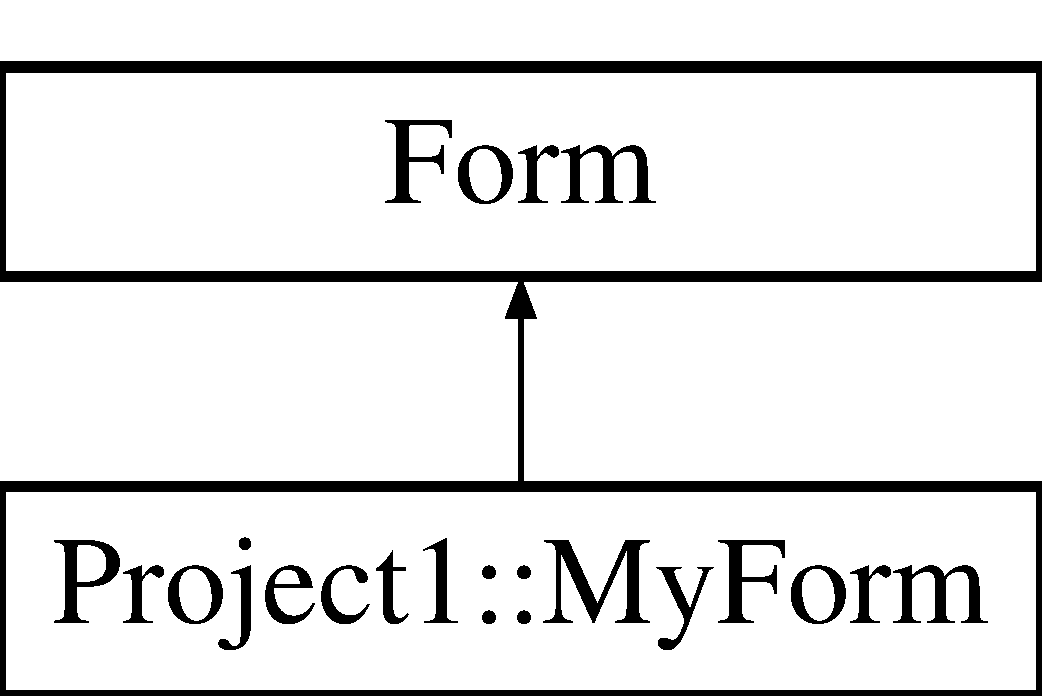
\includegraphics[height=2.000000cm]{class_project1_1_1_my_form}
\end{center}
\end{figure}
\subsection*{公開メンバ関数}
\begin{DoxyCompactItemize}
\item 
\mbox{\Hypertarget{class_project1_1_1_my_form_a2d96004e6380e1bdfffe4675083b6769}\label{class_project1_1_1_my_form_a2d96004e6380e1bdfffe4675083b6769}} 
{\bfseries My\+Form} (clx\+::ini $\ast$Setting\+\_\+, \hyperlink{class_t_k_s_h_o_t}{T\+K\+S\+H\+OT} $\ast$this\+Shot\+\_\+, \hyperlink{class_t_k_p_l_o_t}{T\+K\+P\+L\+OT} $\ast$this\+Plot\+\_\+, \hyperlink{class_t_k_a_d_c_c_o_n_t_r_o_l___d_l750}{T\+K\+A\+D\+C\+C\+O\+N\+T\+R\+O\+L\+\_\+\+D\+L750} $\ast$D\+L750\+\_\+, \hyperlink{class_t_k_a_d_c_c_o_n_t_r_o_l___d_l850}{T\+K\+A\+D\+C\+C\+O\+N\+T\+R\+O\+L\+\_\+\+D\+L850} $\ast$D\+L850\+\_\+)
\end{DoxyCompactItemize}
\subsection*{限定公開メンバ関数}
\begin{DoxyCompactItemize}
\item 
\hyperlink{class_project1_1_1_my_form_a501b2b4481b72877fc73101f1d6f26be}{$\sim$\+My\+Form} ()
\begin{DoxyCompactList}\small\item\em 使用中のリソースをすべてクリーンアップします。 \end{DoxyCompactList}\end{DoxyCompactItemize}


\subsection{詳解}
\hyperlink{class_project1_1_1_my_form}{My\+Form} の概要 



\subsection{構築子と解体子}
\mbox{\Hypertarget{class_project1_1_1_my_form_a501b2b4481b72877fc73101f1d6f26be}\label{class_project1_1_1_my_form_a501b2b4481b72877fc73101f1d6f26be}} 
\index{Project1\+::\+My\+Form@{Project1\+::\+My\+Form}!````~My\+Form@{$\sim$\+My\+Form}}
\index{````~My\+Form@{$\sim$\+My\+Form}!Project1\+::\+My\+Form@{Project1\+::\+My\+Form}}
\subsubsection{\texorpdfstring{$\sim$\+My\+Form()}{~MyForm()}}
{\footnotesize\ttfamily Project1\+::\+My\+Form\+::$\sim$\+My\+Form (\begin{DoxyParamCaption}{ }\end{DoxyParamCaption})\hspace{0.3cm}{\ttfamily [inline]}, {\ttfamily [protected]}}



使用中のリソースをすべてクリーンアップします。 



このクラス詳解は次のファイルから抽出されました\+:\begin{DoxyCompactItemize}
\item 
U\+I/\+Project1/My\+Form.\+h\item 
U\+I/\+Project1/My\+Form.\+cpp\end{DoxyCompactItemize}

\hypertarget{class_t_k_p_l_o_t_1_1_p_l_o_t_i_n_f_o}{}\section{T\+K\+P\+L\+OT\+:\+:P\+L\+O\+T\+I\+N\+FO クラス}
\label{class_t_k_p_l_o_t_1_1_p_l_o_t_i_n_f_o}\index{T\+K\+P\+L\+O\+T\+::\+P\+L\+O\+T\+I\+N\+FO@{T\+K\+P\+L\+O\+T\+::\+P\+L\+O\+T\+I\+N\+FO}}


{\ttfamily \#include $<$tkplot.\+h$>$}

\subsection*{公開メンバ関数}
\begin{DoxyCompactItemize}
\item 
std\+::string \hyperlink{class_t_k_p_l_o_t_1_1_p_l_o_t_i_n_f_o_aa5593f16a8756e42b0ba5e82f79ffd11}{Generate\+Plot\+File\+Name} (const std\+::string prefix)
\begin{DoxyCompactList}\small\item\em gnuplotのコマンドファイルの、拡張子を除いたファイルパスを生成します。出力されるグラフのファイルパスも同じパスとなります。~\newline
同時に plot\+\_\+file\+\_\+nameを初期化します。 \end{DoxyCompactList}\item 
unsigned int \hyperlink{class_t_k_p_l_o_t_1_1_p_l_o_t_i_n_f_o_aba014d5ce5807ab0e1c1a2bfb2aca7dd}{Calc\+Every\+Value} (const unsigned int point\+\_\+per\+\_\+pixel)
\begin{DoxyCompactList}\small\item\em グラフ情報を元にファイルデータの間引き量を計算します。~\newline
同時に everyを初期化します。 \end{DoxyCompactList}\end{DoxyCompactItemize}
\subsection*{公開変数類}
\begin{DoxyCompactItemize}
\item 
\mbox{\Hypertarget{class_t_k_p_l_o_t_1_1_p_l_o_t_i_n_f_o_ac1dae6b6cd429f4276f5a4491af8c24d}\label{class_t_k_p_l_o_t_1_1_p_l_o_t_i_n_f_o_ac1dae6b6cd429f4276f5a4491af8c24d}} 
std\+::string \hyperlink{class_t_k_p_l_o_t_1_1_p_l_o_t_i_n_f_o_ac1dae6b6cd429f4276f5a4491af8c24d}{plot\+\_\+file\+\_\+name}
\begin{DoxyCompactList}\small\item\em gnuplotのコマンドファイルの、拡張子を除いたファイルパスです。出力されるグラフのファイルパスも同じパスとなります。~\newline
 データファイルの拡張子は.\+pltとなります。~\newline
 \hyperlink{class_t_k_p_l_o_t_1_1_p_l_o_t_i_n_f_o_aa5593f16a8756e42b0ba5e82f79ffd11}{Generate\+Plot\+File\+Name()}によって自動的に初期化されます。 \end{DoxyCompactList}\item 
\mbox{\Hypertarget{class_t_k_p_l_o_t_1_1_p_l_o_t_i_n_f_o_ad8458a0719e051e6e3ee9166fffbf311}\label{class_t_k_p_l_o_t_1_1_p_l_o_t_i_n_f_o_ad8458a0719e051e6e3ee9166fffbf311}} 
std\+::string {\bfseries out\+\_\+file\+\_\+name}
\item 
std\+::string \hyperlink{class_t_k_p_l_o_t_1_1_p_l_o_t_i_n_f_o_a18a67313f8bb54564f35f6e6eddef899}{data\+\_\+file\+\_\+name}
\begin{DoxyCompactList}\small\item\em プロットすべきデータファイルの、拡張子を除いたファイルパスです。絶対参照、相対参照ともに使えます。~\newline
 データファイルの拡張子は、\+A\+S\+C\+I\+Iの場合.\+C\+S\+V、バイナリの場合.\+W\+V\+Fである必要があります。 \end{DoxyCompactList}\item 
\mbox{\Hypertarget{class_t_k_p_l_o_t_1_1_p_l_o_t_i_n_f_o_a027ef6fcbaf4b3356926d853e2223e64}\label{class_t_k_p_l_o_t_1_1_p_l_o_t_i_n_f_o_a027ef6fcbaf4b3356926d853e2223e64}} 
int \hyperlink{class_t_k_p_l_o_t_1_1_p_l_o_t_i_n_f_o_a027ef6fcbaf4b3356926d853e2223e64}{data\+\_\+index}
\begin{DoxyCompactList}\small\item\em T\+K\+S\+H\+O\+Tに格納された全\+A\+D\+C、全トレースのデータを順番に並べたときのトレースの番号です。 data\+\_\+indexは一意なトレースを指します。 \end{DoxyCompactList}\item 
int \hyperlink{class_t_k_p_l_o_t_1_1_p_l_o_t_i_n_f_o_a48ef8281322bf15a1e48cca923d34eeb}{trace\+\_\+index}
\begin{DoxyCompactList}\small\item\em そのトレースが含まれる\+A\+D\+Cの、全トレースのデータを順番に並べたときのトレースの番号です。 trace\+\_\+indexはその\+A\+D\+Cにおいて一意なトレースを指します。 \end{DoxyCompactList}\item 
\mbox{\Hypertarget{class_t_k_p_l_o_t_1_1_p_l_o_t_i_n_f_o_a54f1fba1318e3fdb099900839253777e}\label{class_t_k_p_l_o_t_1_1_p_l_o_t_i_n_f_o_a54f1fba1318e3fdb099900839253777e}} 
int \hyperlink{class_t_k_p_l_o_t_1_1_p_l_o_t_i_n_f_o_a54f1fba1318e3fdb099900839253777e}{data\+\_\+source\+\_\+point\+\_\+number}
\begin{DoxyCompactList}\small\item\em データファイルの1列あたりのデータ点数です。 \end{DoxyCompactList}\item 
\mbox{\Hypertarget{class_t_k_p_l_o_t_1_1_p_l_o_t_i_n_f_o_acd0e9a0e12d7679f93004dcb6bbaa489}\label{class_t_k_p_l_o_t_1_1_p_l_o_t_i_n_f_o_acd0e9a0e12d7679f93004dcb6bbaa489}} 
int \hyperlink{class_t_k_p_l_o_t_1_1_p_l_o_t_i_n_f_o_acd0e9a0e12d7679f93004dcb6bbaa489}{point\+\_\+number}
\begin{DoxyCompactList}\small\item\em 最終的に描画される1列あたりのデータ点数です。 \end{DoxyCompactList}\item 
\mbox{\Hypertarget{class_t_k_p_l_o_t_1_1_p_l_o_t_i_n_f_o_a8f7e0649b327f69db18c9bac7315a4e7}\label{class_t_k_p_l_o_t_1_1_p_l_o_t_i_n_f_o_a8f7e0649b327f69db18c9bac7315a4e7}} 
\hyperlink{class_t_k_p_l_o_t_a28dfea1dd78dfc49c1926518da615bfa}{D\+A\+T\+A\+S\+O\+U\+R\+CE} \hyperlink{class_t_k_p_l_o_t_1_1_p_l_o_t_i_n_f_o_a8f7e0649b327f69db18c9bac7315a4e7}{data\+\_\+source}
\begin{DoxyCompactList}\small\item\em ファイルデータのデータ形式を指定します。指定できるデータ形式は D\+A\+T\+A\+S\+O\+U\+R\+C\+Eを参照してくださいs。 \end{DoxyCompactList}\item 
\mbox{\Hypertarget{class_t_k_p_l_o_t_1_1_p_l_o_t_i_n_f_o_a13b0235f3544b9d875af92ce3ac247ab}\label{class_t_k_p_l_o_t_1_1_p_l_o_t_i_n_f_o_a13b0235f3544b9d875af92ce3ac247ab}} 
\hyperlink{class_t_k_p_l_o_t_1_1_r_a_n_g_e}{T\+K\+P\+L\+O\+T\+::\+R\+A\+N\+GE}$<$ float $>$ \hyperlink{class_t_k_p_l_o_t_1_1_p_l_o_t_i_n_f_o_a13b0235f3544b9d875af92ce3ac247ab}{xrange}
\begin{DoxyCompactList}\small\item\em 描画される、あるいは描画された、グラフのx軸の領域です。 \end{DoxyCompactList}\item 
\mbox{\Hypertarget{class_t_k_p_l_o_t_1_1_p_l_o_t_i_n_f_o_a5ce7809252eb582e3fae0a554bcdb65d}\label{class_t_k_p_l_o_t_1_1_p_l_o_t_i_n_f_o_a5ce7809252eb582e3fae0a554bcdb65d}} 
\hyperlink{class_t_k_p_l_o_t_1_1_r_a_n_g_e}{T\+K\+P\+L\+O\+T\+::\+R\+A\+N\+GE}$<$ float $>$ \hyperlink{class_t_k_p_l_o_t_1_1_p_l_o_t_i_n_f_o_a5ce7809252eb582e3fae0a554bcdb65d}{yrange}
\begin{DoxyCompactList}\small\item\em 描画される、あるいは描画された、グラフのy軸の領域です。 \end{DoxyCompactList}\item 
\mbox{\Hypertarget{class_t_k_p_l_o_t_1_1_p_l_o_t_i_n_f_o_a9b6c85908a1a6d8ab8371ea75aec8902}\label{class_t_k_p_l_o_t_1_1_p_l_o_t_i_n_f_o_a9b6c85908a1a6d8ab8371ea75aec8902}} 
unsigned int \hyperlink{class_t_k_p_l_o_t_1_1_p_l_o_t_i_n_f_o_a9b6c85908a1a6d8ab8371ea75aec8902}{every} = 0
\begin{DoxyCompactList}\small\item\em データの間引き量です。データファイルのevery点に対して1点の描画を行います。 \end{DoxyCompactList}\item 
std\+::string \hyperlink{class_t_k_p_l_o_t_1_1_p_l_o_t_i_n_f_o_ae98bf84fdf14074b4f7804f0617aa902}{model\+\_\+name}
\begin{DoxyCompactList}\small\item\em A\+D\+Cのモデル名です。 T\+K\+S\+H\+O\+Tのインスタンスと同じです。 \end{DoxyCompactList}\item 
int \hyperlink{class_t_k_p_l_o_t_1_1_p_l_o_t_i_n_f_o_a801d16eb357241d4f4eeef8c6393bbc4}{channel\+\_\+number}
\begin{DoxyCompactList}\small\item\em チャンネル番号です。 T\+K\+S\+H\+O\+Tのインスタンスと同じです。 \end{DoxyCompactList}\item 
\mbox{\Hypertarget{class_t_k_p_l_o_t_1_1_p_l_o_t_i_n_f_o_afe6df040b952e6ab1e234d17de6023d0}\label{class_t_k_p_l_o_t_1_1_p_l_o_t_i_n_f_o_afe6df040b952e6ab1e234d17de6023d0}} 
\hyperlink{class_t_k_p_l_o_t_1_1_s_i_z_e}{S\+I\+ZE}$<$ int $>$ \hyperlink{class_t_k_p_l_o_t_1_1_p_l_o_t_i_n_f_o_afe6df040b952e6ab1e234d17de6023d0}{terminal\+\_\+size}
\begin{DoxyCompactList}\small\item\em 描画されるグラフの、余白を含めた1枚の大きさです。 \end{DoxyCompactList}\item 
\mbox{\Hypertarget{class_t_k_p_l_o_t_1_1_p_l_o_t_i_n_f_o_a27451bd9ddcd548bff9f91cdda6ed812}\label{class_t_k_p_l_o_t_1_1_p_l_o_t_i_n_f_o_a27451bd9ddcd548bff9f91cdda6ed812}} 
\hyperlink{class_t_k_p_l_o_t_1_1_s_i_z_e}{S\+I\+ZE}$<$ int $>$ \hyperlink{class_t_k_p_l_o_t_1_1_p_l_o_t_i_n_f_o_a27451bd9ddcd548bff9f91cdda6ed812}{drawing\+\_\+size}
\begin{DoxyCompactList}\small\item\em 描画されるグラフの、グラフが描画される部分の大きさです。 \end{DoxyCompactList}\item 
\mbox{\Hypertarget{class_t_k_p_l_o_t_1_1_p_l_o_t_i_n_f_o_ad5e1f688a044784cf24846d04fd48116}\label{class_t_k_p_l_o_t_1_1_p_l_o_t_i_n_f_o_ad5e1f688a044784cf24846d04fd48116}} 
\hyperlink{class_t_k_p_l_o_t_1_1_p_o_s_i_t_i_o_n}{P\+O\+S\+I\+T\+I\+ON}$<$ int $>$ \hyperlink{class_t_k_p_l_o_t_1_1_p_l_o_t_i_n_f_o_ad5e1f688a044784cf24846d04fd48116}{drawing\+\_\+origin}
\begin{DoxyCompactList}\small\item\em 描画されるグラフの、グラフが描画される部分の基点座標です。 \end{DoxyCompactList}\item 
\mbox{\Hypertarget{class_t_k_p_l_o_t_1_1_p_l_o_t_i_n_f_o_a4266fd64b26c45e727843dc017ba2a3d}\label{class_t_k_p_l_o_t_1_1_p_l_o_t_i_n_f_o_a4266fd64b26c45e727843dc017ba2a3d}} 
std\+::vector$<$ \hyperlink{class_t_k_p_l_o_t_1_1_p_o_s_i_t_i_o_n}{P\+O\+S\+I\+T\+I\+ON}$<$ float $>$ $>$ \hyperlink{class_t_k_p_l_o_t_1_1_p_l_o_t_i_n_f_o_a4266fd64b26c45e727843dc017ba2a3d}{label\+\_\+position}
\begin{DoxyCompactList}\small\item\em 描画されるグラフの、ラベル描画の基点座標です。 \end{DoxyCompactList}\end{DoxyCompactItemize}


\subsection{詳解}
\begin{DoxyRefDesc}{todo}
\item[\hyperlink{todo__todo000004}{todo}]ショット情報に関する\+P\+L\+O\+T\+I\+N\+F\+Oインスタンスは廃止し、\+T\+K\+S\+H\+O\+Tを直接参照する \end{DoxyRefDesc}


プロット情報クラス

プロット情報クラスはグラフの描画に必要な情報を集めたクラスです。 

\subsection{関数詳解}
\mbox{\Hypertarget{class_t_k_p_l_o_t_1_1_p_l_o_t_i_n_f_o_aba014d5ce5807ab0e1c1a2bfb2aca7dd}\label{class_t_k_p_l_o_t_1_1_p_l_o_t_i_n_f_o_aba014d5ce5807ab0e1c1a2bfb2aca7dd}} 
\index{T\+K\+P\+L\+O\+T\+::\+P\+L\+O\+T\+I\+N\+FO@{T\+K\+P\+L\+O\+T\+::\+P\+L\+O\+T\+I\+N\+FO}!Calc\+Every\+Value@{Calc\+Every\+Value}}
\index{Calc\+Every\+Value@{Calc\+Every\+Value}!T\+K\+P\+L\+O\+T\+::\+P\+L\+O\+T\+I\+N\+FO@{T\+K\+P\+L\+O\+T\+::\+P\+L\+O\+T\+I\+N\+FO}}
\subsubsection{\texorpdfstring{Calc\+Every\+Value()}{CalcEveryValue()}}
{\footnotesize\ttfamily unsigned int T\+K\+P\+L\+O\+T\+::\+P\+L\+O\+T\+I\+N\+F\+O\+::\+Calc\+Every\+Value (\begin{DoxyParamCaption}\item[{const unsigned int}]{point\+\_\+per\+\_\+pixel }\end{DoxyParamCaption})\hspace{0.3cm}{\ttfamily [inline]}}



グラフ情報を元にファイルデータの間引き量を計算します。~\newline
同時に everyを初期化します。 


\begin{DoxyParams}[1]{引数}
\mbox{\tt in}  & {\em point\+\_\+per\+\_\+pixel} & 1ピクセルあたりの描画点数を指定します。 \\
\hline
\end{DoxyParams}
\begin{DoxyReturn}{戻り値}
every 間引き量を返します。 
\end{DoxyReturn}
\mbox{\Hypertarget{class_t_k_p_l_o_t_1_1_p_l_o_t_i_n_f_o_aa5593f16a8756e42b0ba5e82f79ffd11}\label{class_t_k_p_l_o_t_1_1_p_l_o_t_i_n_f_o_aa5593f16a8756e42b0ba5e82f79ffd11}} 
\index{T\+K\+P\+L\+O\+T\+::\+P\+L\+O\+T\+I\+N\+FO@{T\+K\+P\+L\+O\+T\+::\+P\+L\+O\+T\+I\+N\+FO}!Generate\+Plot\+File\+Name@{Generate\+Plot\+File\+Name}}
\index{Generate\+Plot\+File\+Name@{Generate\+Plot\+File\+Name}!T\+K\+P\+L\+O\+T\+::\+P\+L\+O\+T\+I\+N\+FO@{T\+K\+P\+L\+O\+T\+::\+P\+L\+O\+T\+I\+N\+FO}}
\subsubsection{\texorpdfstring{Generate\+Plot\+File\+Name()}{GeneratePlotFileName()}}
{\footnotesize\ttfamily std\+::string T\+K\+P\+L\+O\+T\+::\+P\+L\+O\+T\+I\+N\+F\+O\+::\+Generate\+Plot\+File\+Name (\begin{DoxyParamCaption}\item[{const std\+::string}]{prefix }\end{DoxyParamCaption})\hspace{0.3cm}{\ttfamily [inline]}}



gnuplotのコマンドファイルの、拡張子を除いたファイルパスを生成します。出力されるグラフのファイルパスも同じパスとなります。~\newline
同時に plot\+\_\+file\+\_\+nameを初期化します。 


\begin{DoxyParams}[1]{引数}
\mbox{\tt in}  & {\em prefix} & ファイル先頭に付けるプレフィックスを指定します。 \\
\hline
\end{DoxyParams}
\begin{DoxyReturn}{戻り値}
plot\+\_\+file\+\_\+name 生成されたファイルパスを返します。 
\end{DoxyReturn}


\subsection{メンバ詳解}
\mbox{\Hypertarget{class_t_k_p_l_o_t_1_1_p_l_o_t_i_n_f_o_a801d16eb357241d4f4eeef8c6393bbc4}\label{class_t_k_p_l_o_t_1_1_p_l_o_t_i_n_f_o_a801d16eb357241d4f4eeef8c6393bbc4}} 
\index{T\+K\+P\+L\+O\+T\+::\+P\+L\+O\+T\+I\+N\+FO@{T\+K\+P\+L\+O\+T\+::\+P\+L\+O\+T\+I\+N\+FO}!channel\+\_\+number@{channel\+\_\+number}}
\index{channel\+\_\+number@{channel\+\_\+number}!T\+K\+P\+L\+O\+T\+::\+P\+L\+O\+T\+I\+N\+FO@{T\+K\+P\+L\+O\+T\+::\+P\+L\+O\+T\+I\+N\+FO}}
\subsubsection{\texorpdfstring{channel\+\_\+number}{channel\_number}}
{\footnotesize\ttfamily int T\+K\+P\+L\+O\+T\+::\+P\+L\+O\+T\+I\+N\+F\+O\+::channel\+\_\+number}



チャンネル番号です。 T\+K\+S\+H\+O\+Tのインスタンスと同じです。 

\begin{DoxyRefDesc}{todo}
\item[\hyperlink{todo__todo000007}{todo}]このインスタンスは廃止し、\+T\+K\+S\+H\+O\+Tを直接参照する \end{DoxyRefDesc}
\mbox{\Hypertarget{class_t_k_p_l_o_t_1_1_p_l_o_t_i_n_f_o_a18a67313f8bb54564f35f6e6eddef899}\label{class_t_k_p_l_o_t_1_1_p_l_o_t_i_n_f_o_a18a67313f8bb54564f35f6e6eddef899}} 
\index{T\+K\+P\+L\+O\+T\+::\+P\+L\+O\+T\+I\+N\+FO@{T\+K\+P\+L\+O\+T\+::\+P\+L\+O\+T\+I\+N\+FO}!data\+\_\+file\+\_\+name@{data\+\_\+file\+\_\+name}}
\index{data\+\_\+file\+\_\+name@{data\+\_\+file\+\_\+name}!T\+K\+P\+L\+O\+T\+::\+P\+L\+O\+T\+I\+N\+FO@{T\+K\+P\+L\+O\+T\+::\+P\+L\+O\+T\+I\+N\+FO}}
\subsubsection{\texorpdfstring{data\+\_\+file\+\_\+name}{data\_file\_name}}
{\footnotesize\ttfamily std\+::string T\+K\+P\+L\+O\+T\+::\+P\+L\+O\+T\+I\+N\+F\+O\+::data\+\_\+file\+\_\+name}



プロットすべきデータファイルの、拡張子を除いたファイルパスです。絶対参照、相対参照ともに使えます。~\newline
 データファイルの拡張子は、\+A\+S\+C\+I\+Iの場合.\+C\+S\+V、バイナリの場合.\+W\+V\+Fである必要があります。 

\begin{DoxyNote}{覚え書き}
データファイルが\+A\+S\+C\+I\+Iの場合、最終的に参照されるのは data\+\_\+file\+\_\+nameの末尾に(大文字の).\+C\+S\+Vを足したファイルになります。この仕様によって、大文字と小文字を区別する(例えば\+Unix系の)環境では data\+\_\+file\+\_\+nameの末尾に(小文字の).\+csvを足したファイルをデータファイルとして参照することはできません。大文字と小文字を区別しない (例えば\+Windowsのような)環境ではどちらか存在する方のファイルが参照される事になります。 

データファイルの拡張子が大文字なのは、横河電機の\+A\+D\+Cの仕様に沿うためです。 
\end{DoxyNote}
\begin{DoxyRefDesc}{todo}
\item[\hyperlink{todo__todo000005}{todo}]このインスタンスは廃止し、\+T\+K\+S\+H\+O\+Tを直接参照する \end{DoxyRefDesc}
\mbox{\Hypertarget{class_t_k_p_l_o_t_1_1_p_l_o_t_i_n_f_o_ae98bf84fdf14074b4f7804f0617aa902}\label{class_t_k_p_l_o_t_1_1_p_l_o_t_i_n_f_o_ae98bf84fdf14074b4f7804f0617aa902}} 
\index{T\+K\+P\+L\+O\+T\+::\+P\+L\+O\+T\+I\+N\+FO@{T\+K\+P\+L\+O\+T\+::\+P\+L\+O\+T\+I\+N\+FO}!model\+\_\+name@{model\+\_\+name}}
\index{model\+\_\+name@{model\+\_\+name}!T\+K\+P\+L\+O\+T\+::\+P\+L\+O\+T\+I\+N\+FO@{T\+K\+P\+L\+O\+T\+::\+P\+L\+O\+T\+I\+N\+FO}}
\subsubsection{\texorpdfstring{model\+\_\+name}{model\_name}}
{\footnotesize\ttfamily std\+::string T\+K\+P\+L\+O\+T\+::\+P\+L\+O\+T\+I\+N\+F\+O\+::model\+\_\+name}



A\+D\+Cのモデル名です。 T\+K\+S\+H\+O\+Tのインスタンスと同じです。 

\begin{DoxyRefDesc}{todo}
\item[\hyperlink{todo__todo000006}{todo}]このインスタンスは廃止し、\+T\+K\+S\+H\+O\+Tを直接参照する \end{DoxyRefDesc}
\mbox{\Hypertarget{class_t_k_p_l_o_t_1_1_p_l_o_t_i_n_f_o_a48ef8281322bf15a1e48cca923d34eeb}\label{class_t_k_p_l_o_t_1_1_p_l_o_t_i_n_f_o_a48ef8281322bf15a1e48cca923d34eeb}} 
\index{T\+K\+P\+L\+O\+T\+::\+P\+L\+O\+T\+I\+N\+FO@{T\+K\+P\+L\+O\+T\+::\+P\+L\+O\+T\+I\+N\+FO}!trace\+\_\+index@{trace\+\_\+index}}
\index{trace\+\_\+index@{trace\+\_\+index}!T\+K\+P\+L\+O\+T\+::\+P\+L\+O\+T\+I\+N\+FO@{T\+K\+P\+L\+O\+T\+::\+P\+L\+O\+T\+I\+N\+FO}}
\subsubsection{\texorpdfstring{trace\+\_\+index}{trace\_index}}
{\footnotesize\ttfamily int T\+K\+P\+L\+O\+T\+::\+P\+L\+O\+T\+I\+N\+F\+O\+::trace\+\_\+index}



そのトレースが含まれる\+A\+D\+Cの、全トレースのデータを順番に並べたときのトレースの番号です。 trace\+\_\+indexはその\+A\+D\+Cにおいて一意なトレースを指します。 

\begin{DoxyNote}{覚え書き}
例えばある\+A\+D\+Cで C\+H2, C\+H5, C\+H8 を用いて計測が行われていたとき、\+C\+H5の trace\+\_\+indexは 1 になります。 

計測器を1台しか用いないショットではdata\+\_\+indexと trace\+\_\+indexの値は等しくなります。 
\end{DoxyNote}


このクラス詳解は次のファイルから抽出されました\+:\begin{DoxyCompactItemize}
\item 
tkplot.\+h\end{DoxyCompactItemize}

\hypertarget{class_t_k_p_l_o_t_1_1_p_o_s_i_t_i_o_n}{}\section{T\+K\+P\+L\+OT\+:\+:P\+O\+S\+I\+T\+I\+ON$<$ T $>$ クラステンプレート}
\label{class_t_k_p_l_o_t_1_1_p_o_s_i_t_i_o_n}\index{T\+K\+P\+L\+O\+T\+::\+P\+O\+S\+I\+T\+I\+O\+N$<$ T $>$@{T\+K\+P\+L\+O\+T\+::\+P\+O\+S\+I\+T\+I\+O\+N$<$ T $>$}}
\subsection*{公開メンバ関数}
\begin{DoxyCompactItemize}
\item 
\mbox{\Hypertarget{class_t_k_p_l_o_t_1_1_p_o_s_i_t_i_o_n_abce2e3b6b659c15133abef1c6e35fe1c}\label{class_t_k_p_l_o_t_1_1_p_o_s_i_t_i_o_n_abce2e3b6b659c15133abef1c6e35fe1c}} 
{\bfseries P\+O\+S\+I\+T\+I\+ON} (T x\+\_\+, T y\+\_\+)
\item 
\mbox{\Hypertarget{class_t_k_p_l_o_t_1_1_p_o_s_i_t_i_o_n_a715ead8ec7884aaca1ec220e77c83b03}\label{class_t_k_p_l_o_t_1_1_p_o_s_i_t_i_o_n_a715ead8ec7884aaca1ec220e77c83b03}} 
std\+::string {\bfseries str} ()
\end{DoxyCompactItemize}
\subsection*{公開変数類}
\begin{DoxyCompactItemize}
\item 
\mbox{\Hypertarget{class_t_k_p_l_o_t_1_1_p_o_s_i_t_i_o_n_a260fc49a5e31e7dd5d42fc01b05a88f7}\label{class_t_k_p_l_o_t_1_1_p_o_s_i_t_i_o_n_a260fc49a5e31e7dd5d42fc01b05a88f7}} 
T {\bfseries x}
\item 
\mbox{\Hypertarget{class_t_k_p_l_o_t_1_1_p_o_s_i_t_i_o_n_ae84c7221f133098571c5389d76285591}\label{class_t_k_p_l_o_t_1_1_p_o_s_i_t_i_o_n_ae84c7221f133098571c5389d76285591}} 
T {\bfseries y}
\item 
\mbox{\Hypertarget{class_t_k_p_l_o_t_1_1_p_o_s_i_t_i_o_n_a023ad2c7a8239540613a5b18c70772ff}\label{class_t_k_p_l_o_t_1_1_p_o_s_i_t_i_o_n_a023ad2c7a8239540613a5b18c70772ff}} 
T \& {\bfseries u} = x
\item 
\mbox{\Hypertarget{class_t_k_p_l_o_t_1_1_p_o_s_i_t_i_o_n_a776d51b19318a7177128c435eae80a48}\label{class_t_k_p_l_o_t_1_1_p_o_s_i_t_i_o_n_a776d51b19318a7177128c435eae80a48}} 
T \& {\bfseries v} = y
\end{DoxyCompactItemize}


このクラス詳解は次のファイルから抽出されました\+:\begin{DoxyCompactItemize}
\item 
tkplot.\+h\end{DoxyCompactItemize}

\hypertarget{class_t_k_p_l_o_t_1_1_r_a_n_g_e}{}\section{T\+K\+P\+L\+OT\+:\+:R\+A\+N\+GE$<$ T $>$ クラステンプレート}
\label{class_t_k_p_l_o_t_1_1_r_a_n_g_e}\index{T\+K\+P\+L\+O\+T\+::\+R\+A\+N\+G\+E$<$ T $>$@{T\+K\+P\+L\+O\+T\+::\+R\+A\+N\+G\+E$<$ T $>$}}
\subsection*{公開メンバ関数}
\begin{DoxyCompactItemize}
\item 
\mbox{\Hypertarget{class_t_k_p_l_o_t_1_1_r_a_n_g_e_a15cccdb1c926b077c9f06173a5d144a5}\label{class_t_k_p_l_o_t_1_1_r_a_n_g_e_a15cccdb1c926b077c9f06173a5d144a5}} 
{\bfseries R\+A\+N\+GE} (T min\+\_\+, T max\+\_\+)
\item 
\mbox{\Hypertarget{class_t_k_p_l_o_t_1_1_r_a_n_g_e_aada3563138773d6575a67eed99dc8c1b}\label{class_t_k_p_l_o_t_1_1_r_a_n_g_e_aada3563138773d6575a67eed99dc8c1b}} 
std\+::string {\bfseries str} ()
\item 
\mbox{\Hypertarget{class_t_k_p_l_o_t_1_1_r_a_n_g_e_ace282f2a0952d3cca69702556ef92836}\label{class_t_k_p_l_o_t_1_1_r_a_n_g_e_ace282f2a0952d3cca69702556ef92836}} 
T {\bfseries median} ()
\end{DoxyCompactItemize}
\subsection*{公開変数類}
\begin{DoxyCompactItemize}
\item 
\mbox{\Hypertarget{class_t_k_p_l_o_t_1_1_r_a_n_g_e_af83dec2420b2e2d8629d212475a49fee}\label{class_t_k_p_l_o_t_1_1_r_a_n_g_e_af83dec2420b2e2d8629d212475a49fee}} 
T {\bfseries min}
\item 
\mbox{\Hypertarget{class_t_k_p_l_o_t_1_1_r_a_n_g_e_a7100fa300f2cffeed4e5f0657afea787}\label{class_t_k_p_l_o_t_1_1_r_a_n_g_e_a7100fa300f2cffeed4e5f0657afea787}} 
T {\bfseries max}
\end{DoxyCompactItemize}


このクラス詳解は次のファイルから抽出されました\+:\begin{DoxyCompactItemize}
\item 
U\+I/\+Project1/tkplot.\+h\end{DoxyCompactItemize}

\hypertarget{class_project1_1_1_setup_a_d_c_connection}{}\section{Project1\+:\+:Setup\+A\+D\+C\+Connection クラス}
\label{class_project1_1_1_setup_a_d_c_connection}\index{Project1\+::\+Setup\+A\+D\+C\+Connection@{Project1\+::\+Setup\+A\+D\+C\+Connection}}


\hyperlink{class_project1_1_1_setup_a_d_c_connection}{Setup\+A\+D\+C\+Connection} �̊\+T�v  




{\ttfamily \#include $<$Setup\+A\+D\+C\+Connection.\+h$>$}

Project1\+:\+:Setup\+A\+D\+C\+Connection の継承関係図\begin{figure}[H]
\begin{center}
\leavevmode
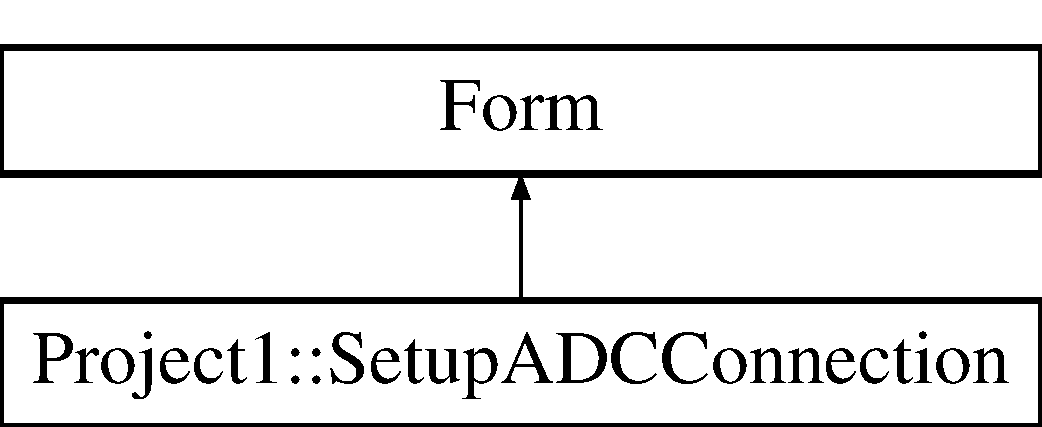
\includegraphics[height=2.000000cm]{class_project1_1_1_setup_a_d_c_connection}
\end{center}
\end{figure}
\subsection*{公開メンバ関数}
\begin{DoxyCompactItemize}
\item 
\mbox{\Hypertarget{class_project1_1_1_setup_a_d_c_connection_ace927052e2be7c56f451eb04559d34d6}\label{class_project1_1_1_setup_a_d_c_connection_ace927052e2be7c56f451eb04559d34d6}} 
{\bfseries Setup\+A\+D\+C\+Connection} (clx\+::ini $\ast$Setting\+\_\+)
\end{DoxyCompactItemize}
\subsection*{限定公開メンバ関数}
\begin{DoxyCompactItemize}
\item 
\hyperlink{class_project1_1_1_setup_a_d_c_connection_a866e7e75c329629e9f2d18ff382a7dc4}{$\sim$\+Setup\+A\+D\+C\+Connection} ()
\begin{DoxyCompactList}\small\item\em �g�p���̃��\textbackslash{}�\mbox{[}�\+X�����ׂă\+N���\mbox{[}���\+A�b�v���܂��B \end{DoxyCompactList}\end{DoxyCompactItemize}


\subsection{詳解}
\hyperlink{class_project1_1_1_setup_a_d_c_connection}{Setup\+A\+D\+C\+Connection} �̊\+T�v 



\subsection{構築子と解体子}
\mbox{\Hypertarget{class_project1_1_1_setup_a_d_c_connection_a866e7e75c329629e9f2d18ff382a7dc4}\label{class_project1_1_1_setup_a_d_c_connection_a866e7e75c329629e9f2d18ff382a7dc4}} 
\index{Project1\+::\+Setup\+A\+D\+C\+Connection@{Project1\+::\+Setup\+A\+D\+C\+Connection}!````~Setup\+A\+D\+C\+Connection@{$\sim$\+Setup\+A\+D\+C\+Connection}}
\index{````~Setup\+A\+D\+C\+Connection@{$\sim$\+Setup\+A\+D\+C\+Connection}!Project1\+::\+Setup\+A\+D\+C\+Connection@{Project1\+::\+Setup\+A\+D\+C\+Connection}}
\subsubsection{\texorpdfstring{$\sim$\+Setup\+A\+D\+C\+Connection()}{~SetupADCConnection()}}
{\footnotesize\ttfamily Project1\+::\+Setup\+A\+D\+C\+Connection\+::$\sim$\+Setup\+A\+D\+C\+Connection (\begin{DoxyParamCaption}{ }\end{DoxyParamCaption})\hspace{0.3cm}{\ttfamily [inline]}, {\ttfamily [protected]}}



�g�p���̃��\textbackslash{}�\mbox{[}�\+X�����ׂă\+N���\mbox{[}���\+A�b�v���܂��B 



このクラス詳解は次のファイルから抽出されました\+:\begin{DoxyCompactItemize}
\item 
Setup\+A\+D\+C\+Connection.\+h\end{DoxyCompactItemize}

\hypertarget{class_project1_1_1_setup_a_d_c_measurement}{}\section{Project1\+:\+:Setup\+A\+D\+C\+Measurement クラス}
\label{class_project1_1_1_setup_a_d_c_measurement}\index{Project1\+::\+Setup\+A\+D\+C\+Measurement@{Project1\+::\+Setup\+A\+D\+C\+Measurement}}


\hyperlink{class_project1_1_1_setup_a_d_c_measurement}{Setup\+A\+D\+C\+Measurement} の概要  




{\ttfamily \#include $<$Setup\+A\+D\+C\+Measurement.\+h$>$}

Project1\+:\+:Setup\+A\+D\+C\+Measurement の継承関係図\begin{figure}[H]
\begin{center}
\leavevmode
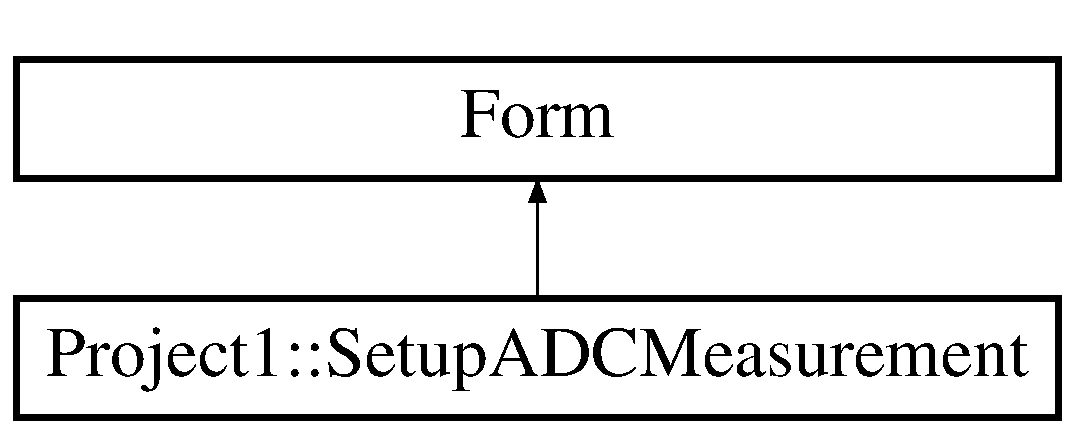
\includegraphics[height=2.000000cm]{class_project1_1_1_setup_a_d_c_measurement}
\end{center}
\end{figure}
\subsection*{限定公開メンバ関数}
\begin{DoxyCompactItemize}
\item 
\hyperlink{class_project1_1_1_setup_a_d_c_measurement_a63b1935cc1f23fc96d175fdb9f1f2fd3}{$\sim$\+Setup\+A\+D\+C\+Measurement} ()
\begin{DoxyCompactList}\small\item\em 使用中のリソースをすべてクリーンアップします。 \end{DoxyCompactList}\end{DoxyCompactItemize}


\subsection{詳解}
\hyperlink{class_project1_1_1_setup_a_d_c_measurement}{Setup\+A\+D\+C\+Measurement} の概要 



\subsection{構築子と解体子}
\mbox{\Hypertarget{class_project1_1_1_setup_a_d_c_measurement_a63b1935cc1f23fc96d175fdb9f1f2fd3}\label{class_project1_1_1_setup_a_d_c_measurement_a63b1935cc1f23fc96d175fdb9f1f2fd3}} 
\index{Project1\+::\+Setup\+A\+D\+C\+Measurement@{Project1\+::\+Setup\+A\+D\+C\+Measurement}!````~Setup\+A\+D\+C\+Measurement@{$\sim$\+Setup\+A\+D\+C\+Measurement}}
\index{````~Setup\+A\+D\+C\+Measurement@{$\sim$\+Setup\+A\+D\+C\+Measurement}!Project1\+::\+Setup\+A\+D\+C\+Measurement@{Project1\+::\+Setup\+A\+D\+C\+Measurement}}
\subsubsection{\texorpdfstring{$\sim$\+Setup\+A\+D\+C\+Measurement()}{~SetupADCMeasurement()}}
{\footnotesize\ttfamily Project1\+::\+Setup\+A\+D\+C\+Measurement\+::$\sim$\+Setup\+A\+D\+C\+Measurement (\begin{DoxyParamCaption}{ }\end{DoxyParamCaption})\hspace{0.3cm}{\ttfamily [inline]}, {\ttfamily [protected]}}



使用中のリソースをすべてクリーンアップします。 



このクラス詳解は次のファイルから抽出されました\+:\begin{DoxyCompactItemize}
\item 
Setup\+A\+D\+C\+Measurement.\+h\end{DoxyCompactItemize}

\hypertarget{class_project1_1_1_setup_analyze_s_p}{}\section{Project1\+:\+:Setup\+Analyze\+SP クラス}
\label{class_project1_1_1_setup_analyze_s_p}\index{Project1\+::\+Setup\+Analyze\+SP@{Project1\+::\+Setup\+Analyze\+SP}}


\hyperlink{class_project1_1_1_setup_analyze_s_p}{Setup\+Analyze\+SP} の概要  




{\ttfamily \#include $<$Setup\+Analyze\+S\+P.\+h$>$}

Project1\+:\+:Setup\+Analyze\+SP の継承関係図\begin{figure}[H]
\begin{center}
\leavevmode
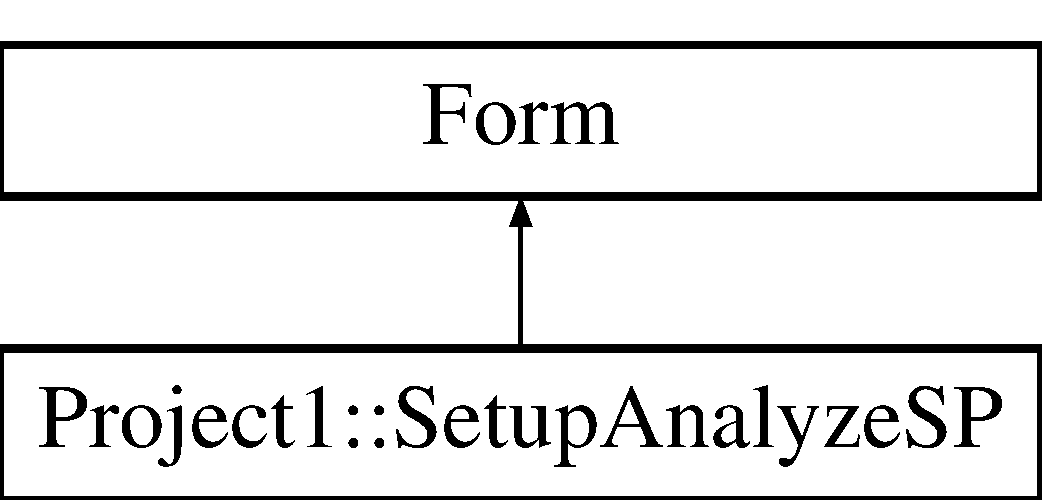
\includegraphics[height=2.000000cm]{class_project1_1_1_setup_analyze_s_p}
\end{center}
\end{figure}
\subsection*{公開メンバ関数}
\begin{DoxyCompactItemize}
\item 
\mbox{\Hypertarget{class_project1_1_1_setup_analyze_s_p_a58fbf31604206da76cead585e94498f2}\label{class_project1_1_1_setup_analyze_s_p_a58fbf31604206da76cead585e94498f2}} 
{\bfseries Setup\+Analyze\+SP} (clx\+::ini $\ast$Setting\+\_\+, \hyperlink{class_t_k_s_h_o_t}{T\+K\+S\+H\+OT} $\ast$this\+Shot\+\_\+, std\+::string group\+\_\+)
\end{DoxyCompactItemize}
\subsection*{限定公開メンバ関数}
\begin{DoxyCompactItemize}
\item 
\hyperlink{class_project1_1_1_setup_analyze_s_p_abb81aeae2341ceec276805a830e94b67}{$\sim$\+Setup\+Analyze\+SP} ()
\begin{DoxyCompactList}\small\item\em 使用中のリソースをすべてクリーンアップします。 \end{DoxyCompactList}\end{DoxyCompactItemize}


\subsection{詳解}
\hyperlink{class_project1_1_1_setup_analyze_s_p}{Setup\+Analyze\+SP} の概要 



\subsection{構築子と解体子}
\mbox{\Hypertarget{class_project1_1_1_setup_analyze_s_p_abb81aeae2341ceec276805a830e94b67}\label{class_project1_1_1_setup_analyze_s_p_abb81aeae2341ceec276805a830e94b67}} 
\index{Project1\+::\+Setup\+Analyze\+SP@{Project1\+::\+Setup\+Analyze\+SP}!````~Setup\+Analyze\+SP@{$\sim$\+Setup\+Analyze\+SP}}
\index{````~Setup\+Analyze\+SP@{$\sim$\+Setup\+Analyze\+SP}!Project1\+::\+Setup\+Analyze\+SP@{Project1\+::\+Setup\+Analyze\+SP}}
\subsubsection{\texorpdfstring{$\sim$\+Setup\+Analyze\+S\+P()}{~SetupAnalyzeSP()}}
{\footnotesize\ttfamily Project1\+::\+Setup\+Analyze\+S\+P\+::$\sim$\+Setup\+Analyze\+SP (\begin{DoxyParamCaption}{ }\end{DoxyParamCaption})\hspace{0.3cm}{\ttfamily [inline]}, {\ttfamily [protected]}}



使用中のリソースをすべてクリーンアップします。 



このクラス詳解は次のファイルから抽出されました\+:\begin{DoxyCompactItemize}
\item 
Setup\+Analyze\+S\+P.\+h\end{DoxyCompactItemize}

\hypertarget{class_project1_1_1_setup_plot}{}\section{Project1\+:\+:Setup\+Plot クラス}
\label{class_project1_1_1_setup_plot}\index{Project1\+::\+Setup\+Plot@{Project1\+::\+Setup\+Plot}}


\hyperlink{class_project1_1_1_setup_plot}{Setup\+Plot} の概要  




{\ttfamily \#include $<$Setup\+Plot.\+h$>$}

Project1\+:\+:Setup\+Plot の継承関係図\begin{figure}[H]
\begin{center}
\leavevmode
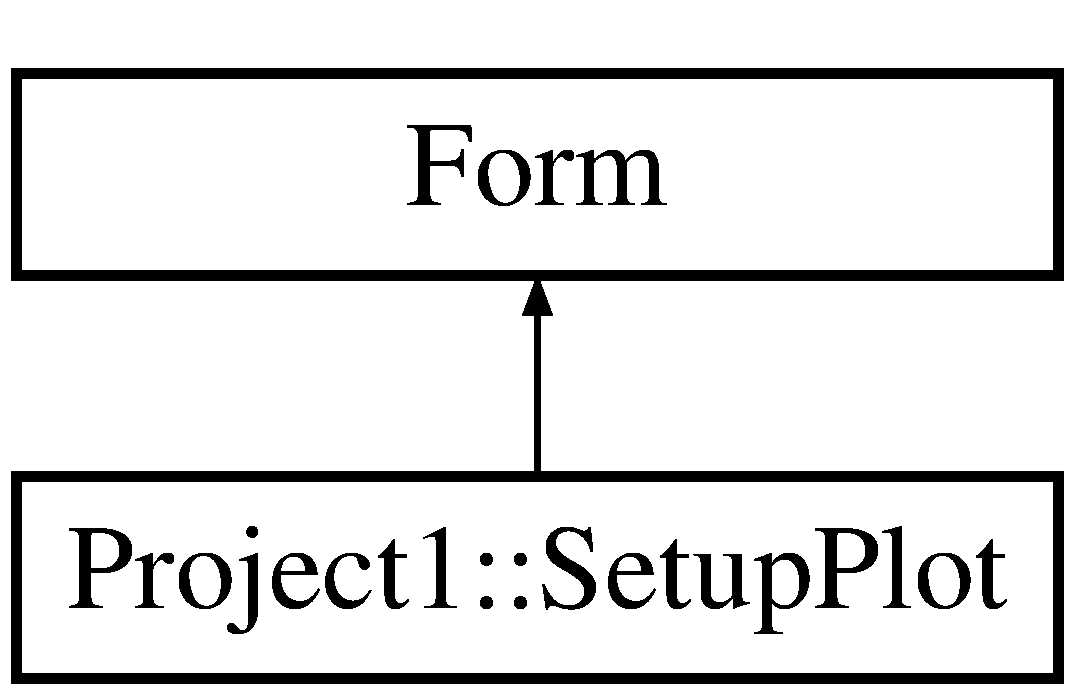
\includegraphics[height=2.000000cm]{class_project1_1_1_setup_plot}
\end{center}
\end{figure}
\subsection*{公開メンバ関数}
\begin{DoxyCompactItemize}
\item 
\mbox{\Hypertarget{class_project1_1_1_setup_plot_a45203c01dce8ca7a6871ff50c10051cd}\label{class_project1_1_1_setup_plot_a45203c01dce8ca7a6871ff50c10051cd}} 
{\bfseries Setup\+Plot} (clx\+::ini $\ast$Shot\+Setting\+\_\+)
\end{DoxyCompactItemize}
\subsection*{限定公開メンバ関数}
\begin{DoxyCompactItemize}
\item 
\hyperlink{class_project1_1_1_setup_plot_a99164cdf31bea63c1f4e01204e381538}{$\sim$\+Setup\+Plot} ()
\begin{DoxyCompactList}\small\item\em 使用中のリソースをすべてクリーンアップします。 \end{DoxyCompactList}\end{DoxyCompactItemize}


\subsection{詳解}
\hyperlink{class_project1_1_1_setup_plot}{Setup\+Plot} の概要 



\subsection{構築子と解体子}
\mbox{\Hypertarget{class_project1_1_1_setup_plot_a99164cdf31bea63c1f4e01204e381538}\label{class_project1_1_1_setup_plot_a99164cdf31bea63c1f4e01204e381538}} 
\index{Project1\+::\+Setup\+Plot@{Project1\+::\+Setup\+Plot}!````~Setup\+Plot@{$\sim$\+Setup\+Plot}}
\index{````~Setup\+Plot@{$\sim$\+Setup\+Plot}!Project1\+::\+Setup\+Plot@{Project1\+::\+Setup\+Plot}}
\subsubsection{\texorpdfstring{$\sim$\+Setup\+Plot()}{~SetupPlot()}}
{\footnotesize\ttfamily Project1\+::\+Setup\+Plot\+::$\sim$\+Setup\+Plot (\begin{DoxyParamCaption}{ }\end{DoxyParamCaption})\hspace{0.3cm}{\ttfamily [inline]}, {\ttfamily [protected]}}



使用中のリソースをすべてクリーンアップします。 



このクラス詳解は次のファイルから抽出されました\+:\begin{DoxyCompactItemize}
\item 
U\+I/\+Project1/Setup\+Plot.\+h\end{DoxyCompactItemize}

\hypertarget{class_t_k_f_i_l_e_u_t_i_l_1_1_s_h_o_t_f_i_l_e_n_a_m_e}{}\section{T\+K\+F\+I\+L\+E\+U\+T\+IL\+:\+:S\+H\+O\+T\+F\+I\+L\+E\+N\+A\+ME クラス}
\label{class_t_k_f_i_l_e_u_t_i_l_1_1_s_h_o_t_f_i_l_e_n_a_m_e}\index{T\+K\+F\+I\+L\+E\+U\+T\+I\+L\+::\+S\+H\+O\+T\+F\+I\+L\+E\+N\+A\+ME@{T\+K\+F\+I\+L\+E\+U\+T\+I\+L\+::\+S\+H\+O\+T\+F\+I\+L\+E\+N\+A\+ME}}
\subsection*{公開メンバ関数}
\begin{DoxyCompactItemize}
\item 
\mbox{\Hypertarget{class_t_k_f_i_l_e_u_t_i_l_1_1_s_h_o_t_f_i_l_e_n_a_m_e_a861f9e8e0995a90ec76f9f256a896edd}\label{class_t_k_f_i_l_e_u_t_i_l_1_1_s_h_o_t_f_i_l_e_n_a_m_e_a861f9e8e0995a90ec76f9f256a896edd}} 
{\bfseries S\+H\+O\+T\+F\+I\+L\+E\+N\+A\+ME} (std\+::string file\+\_\+path\+\_\+)
\item 
\mbox{\Hypertarget{class_t_k_f_i_l_e_u_t_i_l_1_1_s_h_o_t_f_i_l_e_n_a_m_e_a428c708a7e372ff4b4e86e8eff66b3a3}\label{class_t_k_f_i_l_e_u_t_i_l_1_1_s_h_o_t_f_i_l_e_n_a_m_e_a428c708a7e372ff4b4e86e8eff66b3a3}} 
unsigned int \& {\bfseries Shot\+Number} ()
\item 
\mbox{\Hypertarget{class_t_k_f_i_l_e_u_t_i_l_1_1_s_h_o_t_f_i_l_e_n_a_m_e_adc23c9888f4b386bc13232a897b1e08f}\label{class_t_k_f_i_l_e_u_t_i_l_1_1_s_h_o_t_f_i_l_e_n_a_m_e_adc23c9888f4b386bc13232a897b1e08f}} 
std\+::string \& {\bfseries Suffix} ()
\item 
\mbox{\Hypertarget{class_t_k_f_i_l_e_u_t_i_l_1_1_s_h_o_t_f_i_l_e_n_a_m_e_a5feb9f8c9d45ecd63c4a6a3b04d8f0a3}\label{class_t_k_f_i_l_e_u_t_i_l_1_1_s_h_o_t_f_i_l_e_n_a_m_e_a5feb9f8c9d45ecd63c4a6a3b04d8f0a3}} 
std\+::string \& {\bfseries Extension} ()
\item 
\mbox{\Hypertarget{class_t_k_f_i_l_e_u_t_i_l_1_1_s_h_o_t_f_i_l_e_n_a_m_e_a117febf22182245999d54b2275dce157}\label{class_t_k_f_i_l_e_u_t_i_l_1_1_s_h_o_t_f_i_l_e_n_a_m_e_a117febf22182245999d54b2275dce157}} 
std\+::string {\bfseries Get\+File\+Name} ()
\item 
\mbox{\Hypertarget{class_t_k_f_i_l_e_u_t_i_l_1_1_s_h_o_t_f_i_l_e_n_a_m_e_ab86cd404a78edefff8d78910578af6be}\label{class_t_k_f_i_l_e_u_t_i_l_1_1_s_h_o_t_f_i_l_e_n_a_m_e_ab86cd404a78edefff8d78910578af6be}} 
std\+::string {\bfseries Get\+File\+Name\+With\+Extension} ()
\item 
\mbox{\Hypertarget{class_t_k_f_i_l_e_u_t_i_l_1_1_s_h_o_t_f_i_l_e_n_a_m_e_a018228026b6c0bdc2f7e50d084c58393}\label{class_t_k_f_i_l_e_u_t_i_l_1_1_s_h_o_t_f_i_l_e_n_a_m_e_a018228026b6c0bdc2f7e50d084c58393}} 
std\+::string {\bfseries Get\+Directory} ()
\item 
\mbox{\Hypertarget{class_t_k_f_i_l_e_u_t_i_l_1_1_s_h_o_t_f_i_l_e_n_a_m_e_adecbef97489eafba083b43e5118e11ce}\label{class_t_k_f_i_l_e_u_t_i_l_1_1_s_h_o_t_f_i_l_e_n_a_m_e_adecbef97489eafba083b43e5118e11ce}} 
std\+::string {\bfseries Get\+File\+Path} ()
\end{DoxyCompactItemize}


このクラス詳解は次のファイルから抽出されました\+:\begin{DoxyCompactItemize}
\item 
\hyperlink{tkfileutil_8h}{tkfileutil.\+h}\item 
tkfileutil.\+cpp\end{DoxyCompactItemize}

\hypertarget{class_t_k_p_l_o_t_1_1_s_i_z_e}{}\section{T\+K\+P\+L\+OT\+:\+:S\+I\+ZE$<$ T $>$ クラステンプレート}
\label{class_t_k_p_l_o_t_1_1_s_i_z_e}\index{T\+K\+P\+L\+O\+T\+::\+S\+I\+Z\+E$<$ T $>$@{T\+K\+P\+L\+O\+T\+::\+S\+I\+Z\+E$<$ T $>$}}
\subsection*{公開メンバ関数}
\begin{DoxyCompactItemize}
\item 
\mbox{\Hypertarget{class_t_k_p_l_o_t_1_1_s_i_z_e_a876e32d89a46cb96f9020c699b43b9ed}\label{class_t_k_p_l_o_t_1_1_s_i_z_e_a876e32d89a46cb96f9020c699b43b9ed}} 
std\+::string {\bfseries str} ()
\end{DoxyCompactItemize}
\subsection*{公開変数類}
\begin{DoxyCompactItemize}
\item 
\mbox{\Hypertarget{class_t_k_p_l_o_t_1_1_s_i_z_e_a11e6a0ae01e934f1f03cd091a778a4f7}\label{class_t_k_p_l_o_t_1_1_s_i_z_e_a11e6a0ae01e934f1f03cd091a778a4f7}} 
T {\bfseries w}
\item 
\mbox{\Hypertarget{class_t_k_p_l_o_t_1_1_s_i_z_e_af53c6cc5ae8485c0e5842ce59783d39e}\label{class_t_k_p_l_o_t_1_1_s_i_z_e_af53c6cc5ae8485c0e5842ce59783d39e}} 
T {\bfseries h}
\item 
\mbox{\Hypertarget{class_t_k_p_l_o_t_1_1_s_i_z_e_ad01852541685a33ee9ac7fb1fbee13bf}\label{class_t_k_p_l_o_t_1_1_s_i_z_e_ad01852541685a33ee9ac7fb1fbee13bf}} 
T \& {\bfseries u} = w
\item 
\mbox{\Hypertarget{class_t_k_p_l_o_t_1_1_s_i_z_e_ac1fb3da1cbaf26656371b68b1f2955a3}\label{class_t_k_p_l_o_t_1_1_s_i_z_e_ac1fb3da1cbaf26656371b68b1f2955a3}} 
T \& {\bfseries v} = h
\end{DoxyCompactItemize}


このクラス詳解は次のファイルから抽出されました\+:\begin{DoxyCompactItemize}
\item 
U\+I/\+Project1/tkplot.\+h\end{DoxyCompactItemize}

\hypertarget{class_t_k_a_d_c_c_o_n_t_r_o_l}{}\section{T\+K\+A\+D\+C\+C\+O\+N\+T\+R\+OL クラス}
\label{class_t_k_a_d_c_c_o_n_t_r_o_l}\index{T\+K\+A\+D\+C\+C\+O\+N\+T\+R\+OL@{T\+K\+A\+D\+C\+C\+O\+N\+T\+R\+OL}}


{\ttfamily \#include $<$tkadc.\+h$>$}

T\+K\+A\+D\+C\+C\+O\+N\+T\+R\+OL の継承関係図\begin{figure}[H]
\begin{center}
\leavevmode
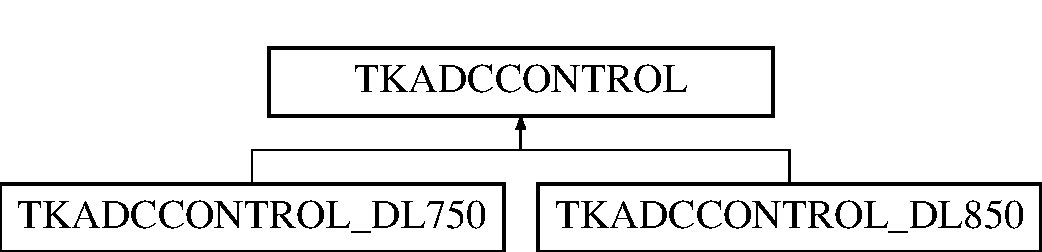
\includegraphics[height=2.000000cm]{class_t_k_a_d_c_c_o_n_t_r_o_l}
\end{center}
\end{figure}
\subsection*{クラス}
\begin{DoxyCompactItemize}
\item 
class \hyperlink{class_t_k_a_d_c_c_o_n_t_r_o_l_1_1_exception}{Exception}
\end{DoxyCompactItemize}
\subsection*{公開型}
\begin{DoxyCompactItemize}
\item 
enum \hyperlink{class_t_k_a_d_c_c_o_n_t_r_o_l_a9a5cfed6c86912f4b9053c8707cf89dd}{A\+D\+C\+M\+O\+D\+EL} \{ {\bfseries D\+L750}, 
{\bfseries D\+L850}
 \}
\item 
enum \hyperlink{class_t_k_a_d_c_c_o_n_t_r_o_l_a4ec8bb3e68a489f7a757d08a855ffb61}{C\+O\+N\+D\+I\+T\+I\+O\+N\+F\+L\+AG} \{ {\bfseries A\+LL} = 0xffff
 \}
\end{DoxyCompactItemize}
\subsection*{公開メンバ関数}
\begin{DoxyCompactItemize}
\item 
\mbox{\Hypertarget{class_t_k_a_d_c_c_o_n_t_r_o_l_a28a8b97f27c62f8bc60f8676f5906320}\label{class_t_k_a_d_c_c_o_n_t_r_o_l_a28a8b97f27c62f8bc60f8676f5906320}} 
{\bfseries T\+K\+A\+D\+C\+C\+O\+N\+T\+R\+OL} (\hyperlink{class_t_k_a_d_c_c_o_n_t_r_o_l_a9a5cfed6c86912f4b9053c8707cf89dd}{A\+D\+C\+M\+O\+D\+EL} adcmodel)
\item 
\mbox{\Hypertarget{class_t_k_a_d_c_c_o_n_t_r_o_l_a1f6c755d05a5d9e3625b6777ccb39ccf}\label{class_t_k_a_d_c_c_o_n_t_r_o_l_a1f6c755d05a5d9e3625b6777ccb39ccf}} 
\hyperlink{class_t_k_a_d_c_c_o_n_t_r_o_l_a9a5cfed6c86912f4b9053c8707cf89dd}{A\+D\+C\+M\+O\+D\+EL} {\bfseries Model} ()
\item 
int \hyperlink{class_t_k_a_d_c_c_o_n_t_r_o_l_a307cc5bd3358c89db6ec7798d47b2840}{Open} (int wire\+\_\+type\+\_\+, const char $\ast$adress\+\_\+)
\item 
int \hyperlink{class_t_k_a_d_c_c_o_n_t_r_o_l_a2f8903ef41b5b97ddf2d2f08a5374402}{Close} ()
\item 
int \hyperlink{class_t_k_a_d_c_c_o_n_t_r_o_l_a2808f2efde28bcfc670d0ddfe2c6791e}{Send\+Message} (const char $\ast$message)
\item 
int \hyperlink{class_t_k_a_d_c_c_o_n_t_r_o_l_afd243c443ca134193acc8a409368aaf3}{Start} ()
\item 
int \hyperlink{class_t_k_a_d_c_c_o_n_t_r_o_l_a3fc45766f6e7f770280f0e165827f86a}{Stop} ()
\item 
int \hyperlink{class_t_k_a_d_c_c_o_n_t_r_o_l_a7d6629217b6f034b9b546f88603d7f58}{Wait\+A\+DC} (\hyperlink{class_t_k_a_d_c_c_o_n_t_r_o_l_a4ec8bb3e68a489f7a757d08a855ffb61}{T\+K\+A\+D\+C\+C\+O\+N\+T\+R\+O\+L\+::\+C\+O\+N\+D\+I\+T\+I\+O\+N\+F\+L\+AG} flag=C\+O\+N\+D\+I\+T\+I\+O\+N\+F\+L\+A\+G\+::\+A\+LL)
\item 
int \hyperlink{class_t_k_a_d_c_c_o_n_t_r_o_l_a832915af5a7240efeef5c3fa139b99af}{Save\+Shot} (std\+::string file\+\_\+name)
\item 
int \hyperlink{class_t_k_a_d_c_c_o_n_t_r_o_l_a63b5da1398f6374705bb5b906e7d23b8}{Get\+Device\+ID} ()
\item 
virtual int \hyperlink{class_t_k_a_d_c_c_o_n_t_r_o_l_ad7009751520eecf10f2fd1aaed28b7df}{Get\+Status\+Condition} (\hyperlink{class_t_k_a_d_c_c_o_n_t_r_o_l_a4ec8bb3e68a489f7a757d08a855ffb61}{T\+K\+A\+D\+C\+C\+O\+N\+T\+R\+O\+L\+::\+C\+O\+N\+D\+I\+T\+I\+O\+N\+F\+L\+AG} flag=C\+O\+N\+D\+I\+T\+I\+O\+N\+F\+L\+A\+G\+::\+A\+LL)
\item 
virtual int \hyperlink{class_t_k_a_d_c_c_o_n_t_r_o_l_afa385509f61162198950676d279f4c3c}{Delete} (std\+::string file\+\_\+name)
\item 
int \hyperlink{class_t_k_a_d_c_c_o_n_t_r_o_l_afbeba1999b1d5afeda2d3b755d20b2ce}{Get\+Last\+Local\+Shot\+Number} ()
\item 
\mbox{\Hypertarget{class_t_k_a_d_c_c_o_n_t_r_o_l_a14b0bfaadfcc3a9e68000da38b34a9ce}\label{class_t_k_a_d_c_c_o_n_t_r_o_l_a14b0bfaadfcc3a9e68000da38b34a9ce}} 
int {\bfseries Get\+Next\+Local\+Shot\+Number} ()
\item 
\mbox{\Hypertarget{class_t_k_a_d_c_c_o_n_t_r_o_l_af2c1452b8d352d610fae97f3f545124b}\label{class_t_k_a_d_c_c_o_n_t_r_o_l_af2c1452b8d352d610fae97f3f545124b}} 
int {\bfseries Set\+Last\+Local\+Shot\+Number} (int new\+\_\+local\+\_\+shot\+\_\+number)
\item 
\mbox{\Hypertarget{class_t_k_a_d_c_c_o_n_t_r_o_l_a424d3c2c41d077dbdc2af5d27e45f76e}\label{class_t_k_a_d_c_c_o_n_t_r_o_l_a424d3c2c41d077dbdc2af5d27e45f76e}} 
int {\bfseries Increment\+Local\+Shot\+Number} ()
\item 
\mbox{\Hypertarget{class_t_k_a_d_c_c_o_n_t_r_o_l_ad75a36e7a3ff1555171addad9dfc1c68}\label{class_t_k_a_d_c_c_o_n_t_r_o_l_ad75a36e7a3ff1555171addad9dfc1c68}} 
int {\bfseries Set\+Local\+Shot\+Number\+Max} (int new\+\_\+local\+\_\+shot\+\_\+number\+\_\+max)
\item 
\mbox{\Hypertarget{class_t_k_a_d_c_c_o_n_t_r_o_l_a997ee62e77c15fc48bf9c7f4deee17f1}\label{class_t_k_a_d_c_c_o_n_t_r_o_l_a997ee62e77c15fc48bf9c7f4deee17f1}} 
int {\bfseries Get\+Local\+Shot\+Number\+Max} ()
\end{DoxyCompactItemize}


\subsection{詳解}
A\+D\+Cコントロールクラス

A\+D\+Cコントロールクラスは\+A\+D\+Cをコントロールするための基底クラスです。~\newline
 A\+D\+Cとのコネクションは排他的であるため、ある\+A\+D\+Cのコントロールには1対1に対応する\+A\+D\+Cコントロールクラスオブジェクトを作成する必要があります。~\newline
 \begin{DoxyParagraph}{この基底クラスが作られた背景}
A\+D\+Cモデルによっては機能が制限されることがあります。例えば\+D\+L750は\+V\+X\+I11に対応していません。\+D\+L1740のコントロールには\+Ethernetを用いることができません。~\newline
 また、\+D\+L750と\+D\+L850のステータスビットの違いのように、\+A\+D\+Cモデルによっては同じ機能でも実装が異なることがあります。~\newline
 このような実装の違いもメソッドをオーバーロードさせることで同様に扱うことができます。~\newline
 
\end{DoxyParagraph}
\begin{DoxyNote}{覚え書き}
もし新たな計測器を追加するようなことがあれば、可能な限り\+A\+D\+Cコントロールクラスを派生させて多態性を持たせてください。 
\end{DoxyNote}


\subsection{列挙型メンバ詳解}
\mbox{\Hypertarget{class_t_k_a_d_c_c_o_n_t_r_o_l_a9a5cfed6c86912f4b9053c8707cf89dd}\label{class_t_k_a_d_c_c_o_n_t_r_o_l_a9a5cfed6c86912f4b9053c8707cf89dd}} 
\index{T\+K\+A\+D\+C\+C\+O\+N\+T\+R\+OL@{T\+K\+A\+D\+C\+C\+O\+N\+T\+R\+OL}!A\+D\+C\+M\+O\+D\+EL@{A\+D\+C\+M\+O\+D\+EL}}
\index{A\+D\+C\+M\+O\+D\+EL@{A\+D\+C\+M\+O\+D\+EL}!T\+K\+A\+D\+C\+C\+O\+N\+T\+R\+OL@{T\+K\+A\+D\+C\+C\+O\+N\+T\+R\+OL}}
\subsubsection{\texorpdfstring{A\+D\+C\+M\+O\+D\+EL}{ADCMODEL}}
{\footnotesize\ttfamily enum \hyperlink{class_t_k_a_d_c_c_o_n_t_r_o_l_a9a5cfed6c86912f4b9053c8707cf89dd}{T\+K\+A\+D\+C\+C\+O\+N\+T\+R\+O\+L\+::\+A\+D\+C\+M\+O\+D\+EL}\hspace{0.3cm}{\ttfamily [strong]}}

A\+D\+Cモデル列挙型

A\+D\+Cのモデルを区別するための型です。~\newline
 A\+D\+Cモデルは多くの場合\+A\+D\+Cの型番を指します(あるいは商品名と呼べるかもしれません)。~\newline
 A\+D\+Cモデルはある\+A\+D\+Cについての固有な名前を意味しません。従って複数の同じ\+A\+D\+Cがシステムに組み込まれている場合は、 それら複数の\+A\+D\+Cが同じ\+A\+D\+Cモデル名を持ちます。~\newline
 A\+D\+Cモデルという呼称は横河電機の流儀に従ったものです。 \mbox{\Hypertarget{class_t_k_a_d_c_c_o_n_t_r_o_l_a4ec8bb3e68a489f7a757d08a855ffb61}\label{class_t_k_a_d_c_c_o_n_t_r_o_l_a4ec8bb3e68a489f7a757d08a855ffb61}} 
\index{T\+K\+A\+D\+C\+C\+O\+N\+T\+R\+OL@{T\+K\+A\+D\+C\+C\+O\+N\+T\+R\+OL}!C\+O\+N\+D\+I\+T\+I\+O\+N\+F\+L\+AG@{C\+O\+N\+D\+I\+T\+I\+O\+N\+F\+L\+AG}}
\index{C\+O\+N\+D\+I\+T\+I\+O\+N\+F\+L\+AG@{C\+O\+N\+D\+I\+T\+I\+O\+N\+F\+L\+AG}!T\+K\+A\+D\+C\+C\+O\+N\+T\+R\+OL@{T\+K\+A\+D\+C\+C\+O\+N\+T\+R\+OL}}
\subsubsection{\texorpdfstring{C\+O\+N\+D\+I\+T\+I\+O\+N\+F\+L\+AG}{CONDITIONFLAG}}
{\footnotesize\ttfamily enum \hyperlink{class_t_k_a_d_c_c_o_n_t_r_o_l_a4ec8bb3e68a489f7a757d08a855ffb61}{T\+K\+A\+D\+C\+C\+O\+N\+T\+R\+O\+L\+::\+C\+O\+N\+D\+I\+T\+I\+O\+N\+F\+L\+AG}\hspace{0.3cm}{\ttfamily [strong]}}

コンディションビットマスク列挙型

ビットマスクはモデルによって異なるため、実際にビットマスクとして使用する為には継承されたクラスで再定義する必要があります。 

\subsection{関数詳解}
\mbox{\Hypertarget{class_t_k_a_d_c_c_o_n_t_r_o_l_a2f8903ef41b5b97ddf2d2f08a5374402}\label{class_t_k_a_d_c_c_o_n_t_r_o_l_a2f8903ef41b5b97ddf2d2f08a5374402}} 
\index{T\+K\+A\+D\+C\+C\+O\+N\+T\+R\+OL@{T\+K\+A\+D\+C\+C\+O\+N\+T\+R\+OL}!Close@{Close}}
\index{Close@{Close}!T\+K\+A\+D\+C\+C\+O\+N\+T\+R\+OL@{T\+K\+A\+D\+C\+C\+O\+N\+T\+R\+OL}}
\subsubsection{\texorpdfstring{Close()}{Close()}}
{\footnotesize\ttfamily T\+K\+A\+D\+C\+C\+O\+N\+T\+R\+O\+L\+::\+Close (\begin{DoxyParamCaption}{ }\end{DoxyParamCaption})}

A\+D\+Cとの通信を閉じます。

デストラクタから呼ばれます。 \begin{DoxyReturn}{戻り値}
0\+: 正常終了 

0以外\+: tmctl.\+hで定義されたエラーコードを返します 
\end{DoxyReturn}
\begin{DoxyNote}{覚え書き}
\hyperlink{class_t_k_a_d_c_c_o_n_t_r_o_l_a2f8903ef41b5b97ddf2d2f08a5374402}{Close()}に失敗すると次の通信が成立しないので、\+Close()できなかった場合は\+A\+D\+Cを再起動させてください。~\newline
 電源の再投入が許されるまでの時間は各\+A\+D\+Cのマニュアルを参照してください。 
\end{DoxyNote}
\mbox{\Hypertarget{class_t_k_a_d_c_c_o_n_t_r_o_l_afa385509f61162198950676d279f4c3c}\label{class_t_k_a_d_c_c_o_n_t_r_o_l_afa385509f61162198950676d279f4c3c}} 
\index{T\+K\+A\+D\+C\+C\+O\+N\+T\+R\+OL@{T\+K\+A\+D\+C\+C\+O\+N\+T\+R\+OL}!Delete@{Delete}}
\index{Delete@{Delete}!T\+K\+A\+D\+C\+C\+O\+N\+T\+R\+OL@{T\+K\+A\+D\+C\+C\+O\+N\+T\+R\+OL}}
\subsubsection{\texorpdfstring{Delete()}{Delete()}}
{\footnotesize\ttfamily T\+K\+A\+D\+C\+C\+O\+N\+T\+R\+O\+L\+::\+Delete (\begin{DoxyParamCaption}\item[{std\+::string}]{file\+\_\+name }\end{DoxyParamCaption})\hspace{0.3cm}{\ttfamily [virtual]}}

A\+D\+Cの内部ストレージから指定したファイル名のバイナリデータを削除します。

存在しないファイル名が指定された場合の挙動は\+A\+D\+Cの仕様によります。 
\begin{DoxyParams}[1]{引数}
\mbox{\tt in}  & {\em file\+\_\+name} & 削除ファイル名を指定します。拡張子は不要です。 \\
\hline
\end{DoxyParams}
\begin{DoxyReturn}{戻り値}
0\+: 正常終了 

0以外\+: tmctl.\+hで定義されたエラーコードを返します 
\end{DoxyReturn}
\begin{DoxyNote}{覚え書き}
D\+L750, D\+L850 では存在しないファイル名が指定された場合、\+A\+D\+Cの画面に警告が出るに留まり、コントロールは継続されます。~\newline
 削除が実行されるとディスクアクセスが発生するため\+Wait\+A\+D\+C()等で待つ必要があります。 
\end{DoxyNote}
\begin{DoxyRefDesc}{todo}
\item[\hyperlink{todo__todo000002}{todo}]許されないファイル名を拒否する \end{DoxyRefDesc}


\hyperlink{class_t_k_a_d_c_c_o_n_t_r_o_l___d_l850_acef79a34544e50a51bab03b83652306a}{T\+K\+A\+D\+C\+C\+O\+N\+T\+R\+O\+L\+\_\+\+D\+L850}, \hyperlink{class_t_k_a_d_c_c_o_n_t_r_o_l___d_l750_a27ce5b790800ffee6d2daddeb0bf9e17}{T\+K\+A\+D\+C\+C\+O\+N\+T\+R\+O\+L\+\_\+\+D\+L750}で再実装されています。

\mbox{\Hypertarget{class_t_k_a_d_c_c_o_n_t_r_o_l_a63b5da1398f6374705bb5b906e7d23b8}\label{class_t_k_a_d_c_c_o_n_t_r_o_l_a63b5da1398f6374705bb5b906e7d23b8}} 
\index{T\+K\+A\+D\+C\+C\+O\+N\+T\+R\+OL@{T\+K\+A\+D\+C\+C\+O\+N\+T\+R\+OL}!Get\+Device\+ID@{Get\+Device\+ID}}
\index{Get\+Device\+ID@{Get\+Device\+ID}!T\+K\+A\+D\+C\+C\+O\+N\+T\+R\+OL@{T\+K\+A\+D\+C\+C\+O\+N\+T\+R\+OL}}
\subsubsection{\texorpdfstring{Get\+Device\+I\+D()}{GetDeviceID()}}
{\footnotesize\ttfamily T\+K\+A\+D\+C\+C\+O\+N\+T\+R\+O\+L\+::\+Get\+Device\+ID (\begin{DoxyParamCaption}\item[{void}]{ }\end{DoxyParamCaption})}

A\+D\+Cとの通信によって生成されるデバイス\+I\+Dを取得します。

通常このデバイス\+I\+Dを知る必要はありません。 \begin{DoxyReturn}{戻り値}
デバイス\+I\+Dを返します 
\end{DoxyReturn}
\mbox{\Hypertarget{class_t_k_a_d_c_c_o_n_t_r_o_l_afbeba1999b1d5afeda2d3b755d20b2ce}\label{class_t_k_a_d_c_c_o_n_t_r_o_l_afbeba1999b1d5afeda2d3b755d20b2ce}} 
\index{T\+K\+A\+D\+C\+C\+O\+N\+T\+R\+OL@{T\+K\+A\+D\+C\+C\+O\+N\+T\+R\+OL}!Get\+Last\+Local\+Shot\+Number@{Get\+Last\+Local\+Shot\+Number}}
\index{Get\+Last\+Local\+Shot\+Number@{Get\+Last\+Local\+Shot\+Number}!T\+K\+A\+D\+C\+C\+O\+N\+T\+R\+OL@{T\+K\+A\+D\+C\+C\+O\+N\+T\+R\+OL}}
\subsubsection{\texorpdfstring{Get\+Last\+Local\+Shot\+Number()}{GetLastLocalShotNumber()}}
{\footnotesize\ttfamily int T\+K\+A\+D\+C\+C\+O\+N\+T\+R\+O\+L\+::\+Get\+Last\+Local\+Shot\+Number (\begin{DoxyParamCaption}{ }\end{DoxyParamCaption})}

\begin{DoxyRefDesc}{todo}
\item[\hyperlink{todo__todo000003}{todo}]A\+D\+Cコントロールクラスに存在するのは不適当なので別のクラスに移動させる \end{DoxyRefDesc}
\mbox{\Hypertarget{class_t_k_a_d_c_c_o_n_t_r_o_l_ad7009751520eecf10f2fd1aaed28b7df}\label{class_t_k_a_d_c_c_o_n_t_r_o_l_ad7009751520eecf10f2fd1aaed28b7df}} 
\index{T\+K\+A\+D\+C\+C\+O\+N\+T\+R\+OL@{T\+K\+A\+D\+C\+C\+O\+N\+T\+R\+OL}!Get\+Status\+Condition@{Get\+Status\+Condition}}
\index{Get\+Status\+Condition@{Get\+Status\+Condition}!T\+K\+A\+D\+C\+C\+O\+N\+T\+R\+OL@{T\+K\+A\+D\+C\+C\+O\+N\+T\+R\+OL}}
\subsubsection{\texorpdfstring{Get\+Status\+Condition()}{GetStatusCondition()}}
{\footnotesize\ttfamily T\+K\+A\+D\+C\+C\+O\+N\+T\+R\+O\+L\+::\+Get\+Status\+Condition (\begin{DoxyParamCaption}\item[{\hyperlink{class_t_k_a_d_c_c_o_n_t_r_o_l_a4ec8bb3e68a489f7a757d08a855ffb61}{T\+K\+A\+D\+C\+C\+O\+N\+T\+R\+O\+L\+::\+C\+O\+N\+D\+I\+T\+I\+O\+N\+F\+L\+AG}}]{flag = {\ttfamily CONDITIONFLAG\+:\+:ALL} }\end{DoxyParamCaption})\hspace{0.3cm}{\ttfamily [virtual]}}

A\+D\+Cのビジー状態を取得します。 
\begin{DoxyParams}[1]{引数}
\mbox{\tt in}  & {\em flag} & ビジー要因のビットマスク条件を指定します。省略した場合は\+C\+O\+N\+D\+I\+T\+I\+O\+N\+F\+L\+A\+G\+::\+A\+L\+Lになります。 \\
\hline
\end{DoxyParams}
\begin{DoxyReturn}{戻り値}
0\+: 指定したビットマスク条件のうちビジー状態のものはありません。 

0以外\+: 指定したビットマスク条件のうち少なくとも1つはビジー状態です。 
\end{DoxyReturn}
\mbox{\Hypertarget{class_t_k_a_d_c_c_o_n_t_r_o_l_a307cc5bd3358c89db6ec7798d47b2840}\label{class_t_k_a_d_c_c_o_n_t_r_o_l_a307cc5bd3358c89db6ec7798d47b2840}} 
\index{T\+K\+A\+D\+C\+C\+O\+N\+T\+R\+OL@{T\+K\+A\+D\+C\+C\+O\+N\+T\+R\+OL}!Open@{Open}}
\index{Open@{Open}!T\+K\+A\+D\+C\+C\+O\+N\+T\+R\+OL@{T\+K\+A\+D\+C\+C\+O\+N\+T\+R\+OL}}
\subsubsection{\texorpdfstring{Open()}{Open()}}
{\footnotesize\ttfamily T\+K\+A\+D\+C\+C\+O\+N\+T\+R\+O\+L\+::\+Open (\begin{DoxyParamCaption}\item[{int}]{wire\+\_\+type\+\_\+,  }\item[{const char $\ast$}]{adress\+\_\+ }\end{DoxyParamCaption})}

A\+D\+Cとの通信を開きます。

開いた通信は\+Close()関数によって必ず閉じる必要があります。 
\begin{DoxyParams}[1]{引数}
\mbox{\tt in}  & {\em wire\+\_\+type\+\_\+} & 通信プロトコルを選択します。 \\
\hline
\mbox{\tt in}  & {\em adress\+\_\+} & アドレスを指定します。 \\
\hline
\end{DoxyParams}
\begin{DoxyReturn}{戻り値}
0\+: 正常終了 

0以外\+: tmctl.\+hで定義されたエラーコードを返します 
\end{DoxyReturn}
\begin{DoxyNote}{覚え書き}
\hyperlink{class_t_k_a_d_c_c_o_n_t_r_o_l_a2f8903ef41b5b97ddf2d2f08a5374402}{Close()}に失敗すると通信が成立しないので、通信が開かない場合は一度\+A\+D\+Cを再起動させてください。 電源の再投入が許されるまでの時間は各\+A\+D\+Cのマニュアルを参照してください。 
\end{DoxyNote}
\mbox{\Hypertarget{class_t_k_a_d_c_c_o_n_t_r_o_l_a832915af5a7240efeef5c3fa139b99af}\label{class_t_k_a_d_c_c_o_n_t_r_o_l_a832915af5a7240efeef5c3fa139b99af}} 
\index{T\+K\+A\+D\+C\+C\+O\+N\+T\+R\+OL@{T\+K\+A\+D\+C\+C\+O\+N\+T\+R\+OL}!Save\+Shot@{Save\+Shot}}
\index{Save\+Shot@{Save\+Shot}!T\+K\+A\+D\+C\+C\+O\+N\+T\+R\+OL@{T\+K\+A\+D\+C\+C\+O\+N\+T\+R\+OL}}
\subsubsection{\texorpdfstring{Save\+Shot()}{SaveShot()}}
{\footnotesize\ttfamily T\+K\+A\+D\+C\+C\+O\+N\+T\+R\+O\+L\+::\+Save\+Shot (\begin{DoxyParamCaption}\item[{std\+::string}]{file\+\_\+name }\end{DoxyParamCaption})}

A\+D\+Cが取り込んだ波形を指定したファイル名で\+A\+D\+Cの内部ストレージに保存します。

バイナリファイルです。既存のファイル名が指定された場合の挙動は\+A\+D\+Cの仕様によります。 
\begin{DoxyParams}[1]{引数}
\mbox{\tt in}  & {\em file\+\_\+name} & 保存ファイル名を指定します。拡張子は不要です。 \\
\hline
\end{DoxyParams}
\begin{DoxyReturn}{戻り値}
0\+: 正常終了 

0以外\+: tmctl.\+hで定義されたエラーコードを返します 
\end{DoxyReturn}
\begin{DoxyWarning}{警告}
D\+L750, D\+L850 ではファイルは上書き保存されず36進数で自動インクリメントされた名前が採用されます。~\newline
 指定した名前と異なるファイルに保存される可能性があることに注意してください。 
\end{DoxyWarning}
\begin{DoxyRefDesc}{todo}
\item[\hyperlink{todo__todo000001}{todo}]保存されたファイル名の取得 

許されないファイル名を拒否する \end{DoxyRefDesc}
\mbox{\Hypertarget{class_t_k_a_d_c_c_o_n_t_r_o_l_a2808f2efde28bcfc670d0ddfe2c6791e}\label{class_t_k_a_d_c_c_o_n_t_r_o_l_a2808f2efde28bcfc670d0ddfe2c6791e}} 
\index{T\+K\+A\+D\+C\+C\+O\+N\+T\+R\+OL@{T\+K\+A\+D\+C\+C\+O\+N\+T\+R\+OL}!Send\+Message@{Send\+Message}}
\index{Send\+Message@{Send\+Message}!T\+K\+A\+D\+C\+C\+O\+N\+T\+R\+OL@{T\+K\+A\+D\+C\+C\+O\+N\+T\+R\+OL}}
\subsubsection{\texorpdfstring{Send\+Message()}{SendMessage()}}
{\footnotesize\ttfamily T\+K\+A\+D\+C\+C\+O\+N\+T\+R\+O\+L\+::\+Send\+Message (\begin{DoxyParamCaption}\item[{const char $\ast$}]{message }\end{DoxyParamCaption})}

A\+D\+Cにメッセージを送信します。

A\+D\+Cをコントロールする手段としては最も低水準な関数です。 
\begin{DoxyParams}[1]{引数}
\mbox{\tt in}  & {\em message} & A\+D\+Cに送信するメッセージを指定します。 \\
\hline
\end{DoxyParams}
\begin{DoxyReturn}{戻り値}
0\+: 正常終了 

0以外\+: tmctl.\+hで定義されたエラーコードを返します 
\end{DoxyReturn}
\mbox{\Hypertarget{class_t_k_a_d_c_c_o_n_t_r_o_l_afd243c443ca134193acc8a409368aaf3}\label{class_t_k_a_d_c_c_o_n_t_r_o_l_afd243c443ca134193acc8a409368aaf3}} 
\index{T\+K\+A\+D\+C\+C\+O\+N\+T\+R\+OL@{T\+K\+A\+D\+C\+C\+O\+N\+T\+R\+OL}!Start@{Start}}
\index{Start@{Start}!T\+K\+A\+D\+C\+C\+O\+N\+T\+R\+OL@{T\+K\+A\+D\+C\+C\+O\+N\+T\+R\+OL}}
\subsubsection{\texorpdfstring{Start()}{Start()}}
{\footnotesize\ttfamily T\+K\+A\+D\+C\+C\+O\+N\+T\+R\+O\+L\+::\+Start (\begin{DoxyParamCaption}{ }\end{DoxyParamCaption})}

A\+D\+Cの計測を開始します。 \begin{DoxyReturn}{戻り値}
0\+: 正常終了 

0以外\+: tmctl.\+hで定義されたエラーコードを返します 
\end{DoxyReturn}
\begin{DoxyNote}{覚え書き}
Singleでの使用を前提としています。 

\hyperlink{class_t_k_a_d_c_c_o_n_t_r_o_l_afd243c443ca134193acc8a409368aaf3}{Start()}が呼ばれた事と\+A\+D\+Cの波形取り込みの準備が整った事(実際に\char`\"{}\+Start\char`\"{}している事)は同義ではありません。~\newline
 例えば\+D\+L850は\+Start()が呼ばれた後、高い頻度でキャリブレーションを実行します。この間波形を取り込むことはできません。~\newline
 波形が取り込める状態かどうかは\+Get\+Status\+Condition(\+T\+K\+A\+D\+C\+C\+O\+N\+T\+R\+O\+L\+::\+C\+O\+N\+D\+I\+T\+I\+O\+N\+F\+L\+A\+G\+::\+T\+R\+G)等で調べる必要があります。 
\end{DoxyNote}
\mbox{\Hypertarget{class_t_k_a_d_c_c_o_n_t_r_o_l_a3fc45766f6e7f770280f0e165827f86a}\label{class_t_k_a_d_c_c_o_n_t_r_o_l_a3fc45766f6e7f770280f0e165827f86a}} 
\index{T\+K\+A\+D\+C\+C\+O\+N\+T\+R\+OL@{T\+K\+A\+D\+C\+C\+O\+N\+T\+R\+OL}!Stop@{Stop}}
\index{Stop@{Stop}!T\+K\+A\+D\+C\+C\+O\+N\+T\+R\+OL@{T\+K\+A\+D\+C\+C\+O\+N\+T\+R\+OL}}
\subsubsection{\texorpdfstring{Stop()}{Stop()}}
{\footnotesize\ttfamily T\+K\+A\+D\+C\+C\+O\+N\+T\+R\+O\+L\+::\+Stop (\begin{DoxyParamCaption}{ }\end{DoxyParamCaption})}

A\+D\+Cの計測を終了します。 \begin{DoxyReturn}{戻り値}
0\+: 正常終了 

0以外\+: tmctl.\+hで定義されたエラーコードを返します 
\end{DoxyReturn}
\mbox{\Hypertarget{class_t_k_a_d_c_c_o_n_t_r_o_l_a7d6629217b6f034b9b546f88603d7f58}\label{class_t_k_a_d_c_c_o_n_t_r_o_l_a7d6629217b6f034b9b546f88603d7f58}} 
\index{T\+K\+A\+D\+C\+C\+O\+N\+T\+R\+OL@{T\+K\+A\+D\+C\+C\+O\+N\+T\+R\+OL}!Wait\+A\+DC@{Wait\+A\+DC}}
\index{Wait\+A\+DC@{Wait\+A\+DC}!T\+K\+A\+D\+C\+C\+O\+N\+T\+R\+OL@{T\+K\+A\+D\+C\+C\+O\+N\+T\+R\+OL}}
\subsubsection{\texorpdfstring{Wait\+A\+D\+C()}{WaitADC()}}
{\footnotesize\ttfamily T\+K\+A\+D\+C\+C\+O\+N\+T\+R\+O\+L\+::\+Wait\+A\+DC (\begin{DoxyParamCaption}\item[{\hyperlink{class_t_k_a_d_c_c_o_n_t_r_o_l_a4ec8bb3e68a489f7a757d08a855ffb61}{T\+K\+A\+D\+C\+C\+O\+N\+T\+R\+O\+L\+::\+C\+O\+N\+D\+I\+T\+I\+O\+N\+F\+L\+AG}}]{flag = {\ttfamily CONDITIONFLAG\+:\+:ALL} }\end{DoxyParamCaption})}

A\+D\+Cがビジー状態の間待ち続けます。 
\begin{DoxyParams}[1]{引数}
\mbox{\tt in}  & {\em flag} & コンディションのビットマスク条件を指定します。省略した場合は\+C\+O\+N\+D\+I\+T\+I\+O\+N\+F\+L\+A\+G\+::\+A\+L\+Lになります。 \\
\hline
\end{DoxyParams}
\begin{DoxyReturn}{戻り値}
0\+: 正常終了 

0以外\+: tmctl.\+hで定義されたエラーコードを返します 
\end{DoxyReturn}


このクラス詳解は次のファイルから抽出されました\+:\begin{DoxyCompactItemize}
\item 
\hyperlink{tkadc_8h}{tkadc.\+h}\item 
tkadc.\+cpp\end{DoxyCompactItemize}

\hypertarget{class_t_k_a_d_c_c_o_n_t_r_o_l___d_l750}{}\section{T\+K\+A\+D\+C\+C\+O\+N\+T\+R\+O\+L\+\_\+\+D\+L750 クラス}
\label{class_t_k_a_d_c_c_o_n_t_r_o_l___d_l750}\index{T\+K\+A\+D\+C\+C\+O\+N\+T\+R\+O\+L\+\_\+\+D\+L750@{T\+K\+A\+D\+C\+C\+O\+N\+T\+R\+O\+L\+\_\+\+D\+L750}}


{\ttfamily \#include $<$tkadc.\+h$>$}

T\+K\+A\+D\+C\+C\+O\+N\+T\+R\+O\+L\+\_\+\+D\+L750 の継承関係図\begin{figure}[H]
\begin{center}
\leavevmode
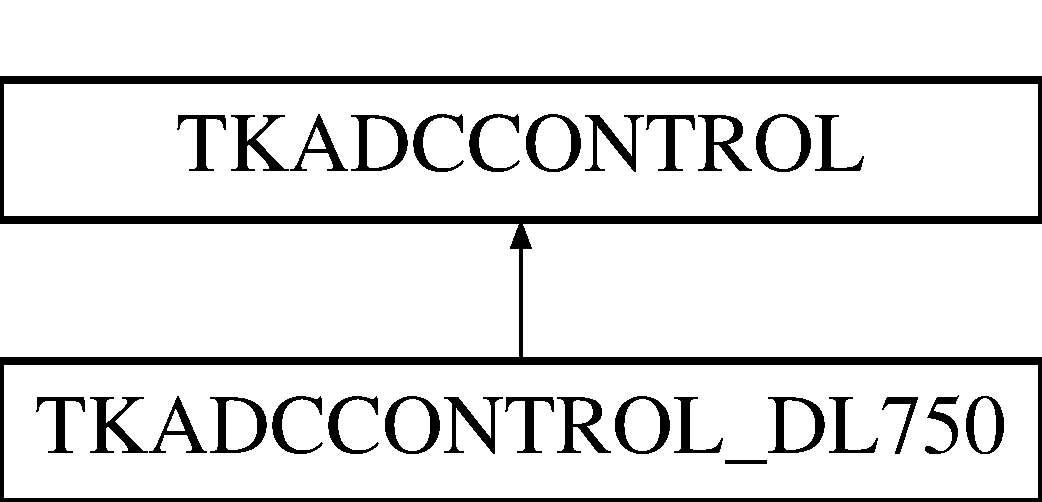
\includegraphics[height=2.000000cm]{class_t_k_a_d_c_c_o_n_t_r_o_l___d_l750}
\end{center}
\end{figure}
\subsection*{公開型}
\begin{DoxyCompactItemize}
\item 
\mbox{\Hypertarget{class_t_k_a_d_c_c_o_n_t_r_o_l___d_l750_a3d102b40e87ea05ca2676ba29ac7fcd3}\label{class_t_k_a_d_c_c_o_n_t_r_o_l___d_l750_a3d102b40e87ea05ca2676ba29ac7fcd3}} 
enum {\bfseries C\+O\+N\+D\+I\+T\+I\+O\+N\+F\+L\+AG} \{ \newline
{\bfseries A\+LL} = 0xffff, 
{\bfseries R\+UN} = 1 $<$$<$ 0, 
{\bfseries T\+RG} = 1 $<$$<$ 2, 
{\bfseries T\+R\+G\+I\+NV} = A\+LL -\/ T\+RG, 
\newline
{\bfseries C\+AL} = 1 $<$$<$ 3, 
{\bfseries T\+ST} = 1 $<$$<$ 4, 
{\bfseries P\+RN} = 1 $<$$<$ 5, 
{\bfseries A\+CS} = 1 $<$$<$ 6, 
\newline
{\bfseries M\+ES} = 1 $<$$<$ 7, 
{\bfseries H\+ST} = 1 $<$$<$ 8, 
{\bfseries S\+UP} = 1 $<$$<$ 9, 
{\bfseries N\+GO} = 1 $<$$<$ 10, 
\newline
{\bfseries S\+CH} = 1 $<$$<$ 11, 
{\bfseries N\+SS} = 1 $<$$<$ 12, 
{\bfseries I\+NI} = 1 $<$$<$ 13, 
{\bfseries F\+FT} = 1 $<$$<$ 14
 \}
\end{DoxyCompactItemize}
\subsection*{公開メンバ関数}
\begin{DoxyCompactItemize}
\item 
\mbox{\Hypertarget{class_t_k_a_d_c_c_o_n_t_r_o_l___d_l750_a446061dc1b932e53ca20d8ae449d788e}\label{class_t_k_a_d_c_c_o_n_t_r_o_l___d_l750_a446061dc1b932e53ca20d8ae449d788e}} 
int {\bfseries Get\+Status\+Condition} (T\+K\+A\+D\+C\+C\+O\+N\+T\+R\+O\+L\+\_\+\+D\+L750\+::\+C\+O\+N\+D\+I\+T\+I\+O\+N\+F\+L\+AG flag=C\+O\+N\+D\+I\+T\+I\+O\+N\+F\+L\+A\+G\+::\+A\+LL)
\item 
int \hyperlink{class_t_k_a_d_c_c_o_n_t_r_o_l___d_l750_a27ce5b790800ffee6d2daddeb0bf9e17}{Delete} (std\+::string file\+\_\+name)
\end{DoxyCompactItemize}


\subsection{詳解}
D\+L750\+A\+D\+Cコントロールクラス

D\+L750をコントロールするためのクラスです。 

\subsection{関数詳解}
\mbox{\Hypertarget{class_t_k_a_d_c_c_o_n_t_r_o_l___d_l750_a27ce5b790800ffee6d2daddeb0bf9e17}\label{class_t_k_a_d_c_c_o_n_t_r_o_l___d_l750_a27ce5b790800ffee6d2daddeb0bf9e17}} 
\index{T\+K\+A\+D\+C\+C\+O\+N\+T\+R\+O\+L\+\_\+\+D\+L750@{T\+K\+A\+D\+C\+C\+O\+N\+T\+R\+O\+L\+\_\+\+D\+L750}!Delete@{Delete}}
\index{Delete@{Delete}!T\+K\+A\+D\+C\+C\+O\+N\+T\+R\+O\+L\+\_\+\+D\+L750@{T\+K\+A\+D\+C\+C\+O\+N\+T\+R\+O\+L\+\_\+\+D\+L750}}
\subsubsection{\texorpdfstring{Delete()}{Delete()}}
{\footnotesize\ttfamily int T\+K\+A\+D\+C\+C\+O\+N\+T\+R\+O\+L\+\_\+\+D\+L750\+::\+Delete (\begin{DoxyParamCaption}\item[{std\+::string}]{file\+\_\+name }\end{DoxyParamCaption})\hspace{0.3cm}{\ttfamily [virtual]}}

A\+D\+Cの内部ストレージから指定したファイル名のバイナリデータを削除します。

存在しないファイル名が指定された場合の挙動は\+A\+D\+Cの仕様によります。 
\begin{DoxyParams}[1]{引数}
\mbox{\tt in}  & {\em file\+\_\+name} & 削除ファイル名を指定します。拡張子は不要です。 \\
\hline
\end{DoxyParams}
\begin{DoxyReturn}{戻り値}
0\+: 正常終了 

0以外\+: tmctl.\+hで定義されたエラーコードを返します 
\end{DoxyReturn}
\begin{DoxyNote}{覚え書き}
D\+L750, D\+L850 では存在しないファイル名が指定された場合、\+A\+D\+Cの画面に警告が出るに留まり、コントロールは継続されます。~\newline
 削除が実行されるとディスクアクセスが発生するため\+Wait\+A\+D\+C()等で待つ必要があります。 
\end{DoxyNote}
\begin{DoxyRefDesc}{todo}
\item[\hyperlink{todo__todo000002}{todo}]許されないファイル名を拒否する \end{DoxyRefDesc}


\hyperlink{class_t_k_a_d_c_c_o_n_t_r_o_l_afa385509f61162198950676d279f4c3c}{T\+K\+A\+D\+C\+C\+O\+N\+T\+R\+OL}を再実装しています。



このクラス詳解は次のファイルから抽出されました\+:\begin{DoxyCompactItemize}
\item 
U\+I/\+Project1/\hyperlink{tkadc_8h}{tkadc.\+h}\item 
U\+I/\+Project1/tkadc.\+cpp\end{DoxyCompactItemize}

\hypertarget{class_t_k_a_d_c_c_o_n_t_r_o_l___d_l850}{}\section{T\+K\+A\+D\+C\+C\+O\+N\+T\+R\+O\+L\+\_\+\+D\+L850 クラス}
\label{class_t_k_a_d_c_c_o_n_t_r_o_l___d_l850}\index{T\+K\+A\+D\+C\+C\+O\+N\+T\+R\+O\+L\+\_\+\+D\+L850@{T\+K\+A\+D\+C\+C\+O\+N\+T\+R\+O\+L\+\_\+\+D\+L850}}


{\ttfamily \#include $<$tkadc.\+h$>$}

T\+K\+A\+D\+C\+C\+O\+N\+T\+R\+O\+L\+\_\+\+D\+L850 の継承関係図\begin{figure}[H]
\begin{center}
\leavevmode
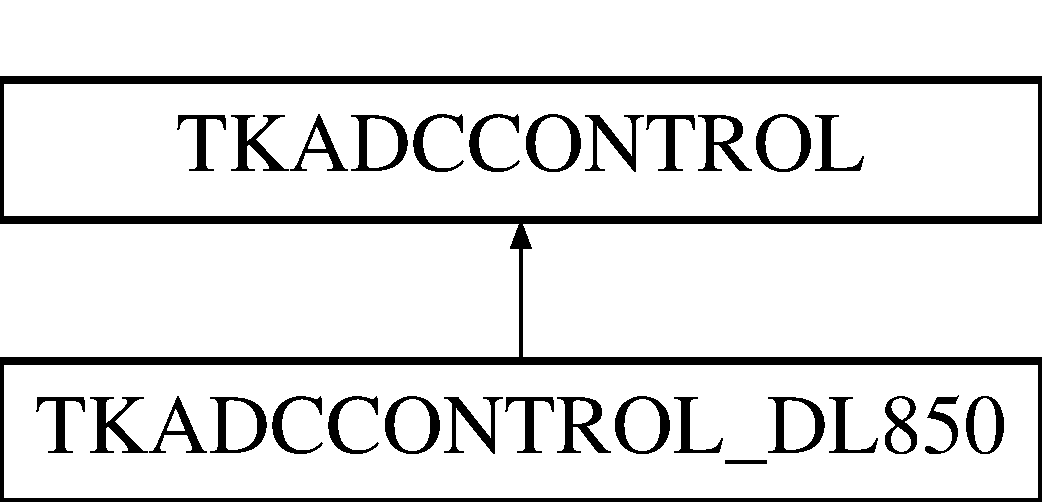
\includegraphics[height=2.000000cm]{class_t_k_a_d_c_c_o_n_t_r_o_l___d_l850}
\end{center}
\end{figure}
\subsection*{公開型}
\begin{DoxyCompactItemize}
\item 
\mbox{\Hypertarget{class_t_k_a_d_c_c_o_n_t_r_o_l___d_l850_aecf0f8f87a3fd72a24a12d859eefd456}\label{class_t_k_a_d_c_c_o_n_t_r_o_l___d_l850_aecf0f8f87a3fd72a24a12d859eefd456}} 
enum {\bfseries C\+O\+N\+D\+I\+T\+I\+O\+N\+F\+L\+AG} \{ \newline
{\bfseries A\+LL} = 0xffff, 
{\bfseries C\+AP} = 1 $<$$<$ 0, 
{\bfseries R\+EC} = 1 $<$$<$ 1, 
{\bfseries T\+RG} = 1 $<$$<$ 2, 
\newline
{\bfseries T\+R\+G\+I\+NV} = A\+LL -\/ T\+RG, 
{\bfseries C\+AL} = 1 $<$$<$ 3, 
{\bfseries T\+ST} = 1 $<$$<$ 4, 
{\bfseries P\+RN} = 1 $<$$<$ 5, 
\newline
{\bfseries A\+CS} = 1 $<$$<$ 6, 
{\bfseries M\+ES} = 1 $<$$<$ 7, 
{\bfseries H\+ST} = 1 $<$$<$ 8, 
{\bfseries C\+NT} = 1 $<$$<$ 9, 
\newline
{\bfseries N\+GO} = 1 $<$$<$ 10, 
{\bfseries S\+CH} = 1 $<$$<$ 11, 
{\bfseries R\+UN} = 1 $<$$<$ 12, 
{\bfseries K\+LK} = 1 $<$$<$ 13, 
\newline
{\bfseries AN} = 1 $<$$<$ 14
 \}
\end{DoxyCompactItemize}
\subsection*{公開メンバ関数}
\begin{DoxyCompactItemize}
\item 
\mbox{\Hypertarget{class_t_k_a_d_c_c_o_n_t_r_o_l___d_l850_aecc88bc7f7ae5b93e578f711ce653e0f}\label{class_t_k_a_d_c_c_o_n_t_r_o_l___d_l850_aecc88bc7f7ae5b93e578f711ce653e0f}} 
int {\bfseries Get\+Status\+Condition} (T\+K\+A\+D\+C\+C\+O\+N\+T\+R\+O\+L\+\_\+\+D\+L850\+::\+C\+O\+N\+D\+I\+T\+I\+O\+N\+F\+L\+AG flag=C\+O\+N\+D\+I\+T\+I\+O\+N\+F\+L\+A\+G\+::\+A\+LL)
\item 
int \hyperlink{class_t_k_a_d_c_c_o_n_t_r_o_l___d_l850_acef79a34544e50a51bab03b83652306a}{Delete} (std\+::string file\+\_\+name)
\end{DoxyCompactItemize}


\subsection{詳解}
D\+L850\+A\+D\+Cコントロールクラス

D\+L850をコントロールするためのクラスです。 

\subsection{関数詳解}
\mbox{\Hypertarget{class_t_k_a_d_c_c_o_n_t_r_o_l___d_l850_acef79a34544e50a51bab03b83652306a}\label{class_t_k_a_d_c_c_o_n_t_r_o_l___d_l850_acef79a34544e50a51bab03b83652306a}} 
\index{T\+K\+A\+D\+C\+C\+O\+N\+T\+R\+O\+L\+\_\+\+D\+L850@{T\+K\+A\+D\+C\+C\+O\+N\+T\+R\+O\+L\+\_\+\+D\+L850}!Delete@{Delete}}
\index{Delete@{Delete}!T\+K\+A\+D\+C\+C\+O\+N\+T\+R\+O\+L\+\_\+\+D\+L850@{T\+K\+A\+D\+C\+C\+O\+N\+T\+R\+O\+L\+\_\+\+D\+L850}}
\subsubsection{\texorpdfstring{Delete()}{Delete()}}
{\footnotesize\ttfamily int T\+K\+A\+D\+C\+C\+O\+N\+T\+R\+O\+L\+\_\+\+D\+L850\+::\+Delete (\begin{DoxyParamCaption}\item[{std\+::string}]{file\+\_\+name }\end{DoxyParamCaption})\hspace{0.3cm}{\ttfamily [virtual]}}

A\+D\+Cの内部ストレージから指定したファイル名のバイナリデータを削除します。

存在しないファイル名が指定された場合の挙動は\+A\+D\+Cの仕様によります。 
\begin{DoxyParams}[1]{引数}
\mbox{\tt in}  & {\em file\+\_\+name} & 削除ファイル名を指定します。拡張子は不要です。 \\
\hline
\end{DoxyParams}
\begin{DoxyReturn}{戻り値}
0\+: 正常終了 

0以外\+: tmctl.\+hで定義されたエラーコードを返します 
\end{DoxyReturn}
\begin{DoxyNote}{覚え書き}
D\+L750, D\+L850 では存在しないファイル名が指定された場合、\+A\+D\+Cの画面に警告が出るに留まり、コントロールは継続されます。~\newline
 削除が実行されるとディスクアクセスが発生するため\+Wait\+A\+D\+C()等で待つ必要があります。 
\end{DoxyNote}
\begin{DoxyRefDesc}{todo}
\item[\hyperlink{todo__todo000002}{todo}]許されないファイル名を拒否する \end{DoxyRefDesc}


\hyperlink{class_t_k_a_d_c_c_o_n_t_r_o_l_afa385509f61162198950676d279f4c3c}{T\+K\+A\+D\+C\+C\+O\+N\+T\+R\+OL}を再実装しています。



このクラス詳解は次のファイルから抽出されました\+:\begin{DoxyCompactItemize}
\item 
U\+I/\+Project1/\hyperlink{tkadc_8h}{tkadc.\+h}\item 
U\+I/\+Project1/tkadc.\+cpp\end{DoxyCompactItemize}

\hypertarget{class_t_k_a_n_a_l_y_z_e}{}\section{T\+K\+A\+N\+A\+L\+Y\+ZE クラス}
\label{class_t_k_a_n_a_l_y_z_e}\index{T\+K\+A\+N\+A\+L\+Y\+ZE@{T\+K\+A\+N\+A\+L\+Y\+ZE}}
T\+K\+A\+N\+A\+L\+Y\+ZE の継承関係図\begin{figure}[H]
\begin{center}
\leavevmode
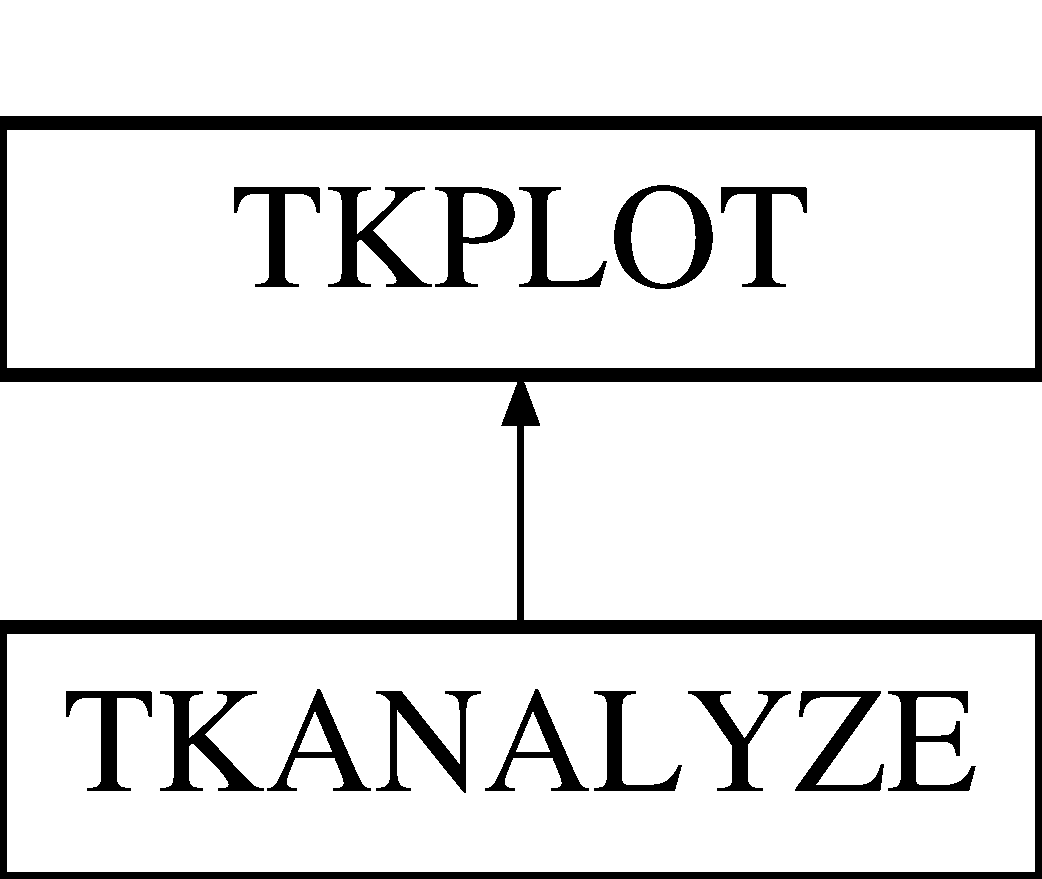
\includegraphics[height=3.000000cm]{class_t_k_a_n_a_l_y_z_e}
\end{center}
\end{figure}
\subsection*{クラス}
\begin{DoxyCompactItemize}
\item 
class \hyperlink{class_t_k_a_n_a_l_y_z_e_1_1_f_i_t_r_a_n_g_e}{F\+I\+T\+R\+A\+N\+GE}
\end{DoxyCompactItemize}
\subsection*{公開型}
\begin{DoxyCompactItemize}
\item 
\mbox{\Hypertarget{class_t_k_a_n_a_l_y_z_e_aaf7dd74ca27bd81681431db1e0bad011}\label{class_t_k_a_n_a_l_y_z_e_aaf7dd74ca27bd81681431db1e0bad011}} 
enum {\bfseries P\+R\+E\+D\+A\+T\+A\+P\+R\+O\+C\+E\+S\+SS} \{ {\bfseries Raw}, 
{\bfseries S\+MA}, 
{\bfseries S\+M\+A\+\_\+\+KH}, 
{\bfseries S\+M\+A\+\_\+\+K\+H\+\_\+\+S\+MA}
 \}
\end{DoxyCompactItemize}
\subsection*{公開メンバ関数}
\begin{DoxyCompactItemize}
\item 
\mbox{\Hypertarget{class_t_k_a_n_a_l_y_z_e_ac522bb7549f5e2329a8de8de2b2b2d8a}\label{class_t_k_a_n_a_l_y_z_e_ac522bb7549f5e2329a8de8de2b2b2d8a}} 
{\bfseries T\+K\+A\+N\+A\+L\+Y\+ZE} (\hyperlink{class_t_k_s_h_o_t}{T\+K\+S\+H\+OT} $\ast$T\+K\+Shot\+\_\+, clx\+::ini $\ast$Setting\+\_\+, std\+::string group\+\_\+)
\item 
\mbox{\Hypertarget{class_t_k_a_n_a_l_y_z_e_a597c5a215fdb450ba3e169c2487cb3ed}\label{class_t_k_a_n_a_l_y_z_e_a597c5a215fdb450ba3e169c2487cb3ed}} 
void {\bfseries Set\+M\+A\+Sample\+Number} (int sample\+\_\+number)
\item 
\mbox{\Hypertarget{class_t_k_a_n_a_l_y_z_e_aae3d430b4ed92bb61177cc8973ff2953}\label{class_t_k_a_n_a_l_y_z_e_aae3d430b4ed92bb61177cc8973ff2953}} 
virtual int {\bfseries Plot\+Analyze\+SP} (\hyperlink{class_t_k_p_l_o_t_a158082ae168750554cf23edde9a27416}{T\+K\+P\+L\+O\+T\+::\+P\+L\+O\+T\+S\+I\+ZE} plot\+\_\+size, int shot\+\_\+number)=0
\item 
\mbox{\Hypertarget{class_t_k_a_n_a_l_y_z_e_abcaf46784a1be43930c1909f5ce122aa}\label{class_t_k_a_n_a_l_y_z_e_abcaf46784a1be43930c1909f5ce122aa}} 
std\+::vector$<$ \hyperlink{class_t_k_p_l_o_t_1_1_p_l_o_t_i_n_f_o}{P\+L\+O\+T\+I\+N\+FO} $>$ {\bfseries Get\+Plot\+Info} ()
\item 
\mbox{\Hypertarget{class_t_k_a_n_a_l_y_z_e_a7a1898bb5c3959ba18cf4b6cb22557a5}\label{class_t_k_a_n_a_l_y_z_e_a7a1898bb5c3959ba18cf4b6cb22557a5}} 
std\+::vector$<$ \hyperlink{class_t_k_p_l_o_t_1_1_p_l_o_t_i_n_f_o}{T\+K\+P\+L\+O\+T\+::\+P\+L\+O\+T\+I\+N\+FO} $>$\+::pointer {\bfseries Get\+Plot\+Info\+Ptr} ()
\item 
\mbox{\Hypertarget{class_t_k_a_n_a_l_y_z_e_aa3c73c920679675b1a99bf2c0a3dfc1b}\label{class_t_k_a_n_a_l_y_z_e_aa3c73c920679675b1a99bf2c0a3dfc1b}} 
\hyperlink{class_t_k_a_n_a_l_y_z_e_1_1_f_i_t_r_a_n_g_e}{F\+I\+T\+R\+A\+N\+GE} \& {\bfseries Set\+Range} ()
\item 
\mbox{\Hypertarget{class_t_k_a_n_a_l_y_z_e_ac46755c0c97570a8b2f9fee8abe0098a}\label{class_t_k_a_n_a_l_y_z_e_ac46755c0c97570a8b2f9fee8abe0098a}} 
double {\bfseries Get\+Start\+Time} ()
\item 
\mbox{\Hypertarget{class_t_k_a_n_a_l_y_z_e_a07e65d7e0e9a7ca58f73432b44541a47}\label{class_t_k_a_n_a_l_y_z_e_a07e65d7e0e9a7ca58f73432b44541a47}} 
double {\bfseries Get\+Stop\+Time} ()
\item 
\mbox{\Hypertarget{class_t_k_a_n_a_l_y_z_e_aa26fd364fff1d69ead56a53d1d2de439}\label{class_t_k_a_n_a_l_y_z_e_aa26fd364fff1d69ead56a53d1d2de439}} 
unsigned int {\bfseries Get\+Start\+Point} (int adc\+\_\+id)
\item 
\mbox{\Hypertarget{class_t_k_a_n_a_l_y_z_e_a561d27047b90eb3a344a1c86f5290605}\label{class_t_k_a_n_a_l_y_z_e_a561d27047b90eb3a344a1c86f5290605}} 
unsigned int {\bfseries Get\+Stop\+Point} (int adc\+\_\+id)
\item 
\mbox{\Hypertarget{class_t_k_a_n_a_l_y_z_e_a607144cda4f6ad2cf472ee792c0aa8a7}\label{class_t_k_a_n_a_l_y_z_e_a607144cda4f6ad2cf472ee792c0aa8a7}} 
unsigned int {\bfseries Get\+One\+Cycle\+Stop\+Point} (int adc\+\_\+id)
\item 
\mbox{\Hypertarget{class_t_k_a_n_a_l_y_z_e_a5be002cc215145a2af05c85cf50aabe7}\label{class_t_k_a_n_a_l_y_z_e_a5be002cc215145a2af05c85cf50aabe7}} 
std\+::string {\bfseries Exec\+Pre\+Data\+Process} (int plot\+\_\+info\+\_\+index)
\end{DoxyCompactItemize}
\subsection*{公開変数類}
\begin{DoxyCompactItemize}
\item 
\mbox{\Hypertarget{class_t_k_a_n_a_l_y_z_e_a55e1a2c600ba6fb90f849f04e3dffc0d}\label{class_t_k_a_n_a_l_y_z_e_a55e1a2c600ba6fb90f849f04e3dffc0d}} 
\hyperlink{class_t_k_a_n_a_l_y_z_e_1_1_f_i_t_r_a_n_g_e}{F\+I\+T\+R\+A\+N\+GE} {\bfseries fitrange}
\item 
\mbox{\Hypertarget{class_t_k_a_n_a_l_y_z_e_a924ebf2dbad843a1daf66c85cdfa4b4a}\label{class_t_k_a_n_a_l_y_z_e_a924ebf2dbad843a1daf66c85cdfa4b4a}} 
P\+R\+E\+D\+A\+T\+A\+P\+R\+O\+C\+E\+S\+SS {\bfseries pre\+\_\+data\+\_\+process}
\end{DoxyCompactItemize}
\subsection*{限定公開メンバ関数}
\begin{DoxyCompactItemize}
\item 
\mbox{\Hypertarget{class_t_k_a_n_a_l_y_z_e_ab3051e2a2012e986b33a97a2389b2f47}\label{class_t_k_a_n_a_l_y_z_e_ab3051e2a2012e986b33a97a2389b2f47}} 
double {\bfseries calc\+Surface\+Area} (T\+K\+Charged\+Particle\+Type particle\+\_\+type)
\end{DoxyCompactItemize}
\subsection*{限定公開変数類}
\begin{DoxyCompactItemize}
\item 
\mbox{\Hypertarget{class_t_k_a_n_a_l_y_z_e_a9413390f419657d838a950ad91198b2d}\label{class_t_k_a_n_a_l_y_z_e_a9413390f419657d838a950ad91198b2d}} 
\hyperlink{class_t_k_s_h_o_t}{T\+K\+S\+H\+OT} $\ast$ {\bfseries this\+Shot}
\item 
\mbox{\Hypertarget{class_t_k_a_n_a_l_y_z_e_a8ef97d5dda7259043e08c5d80dc321d0}\label{class_t_k_a_n_a_l_y_z_e_a8ef97d5dda7259043e08c5d80dc321d0}} 
clx\+::ini $\ast$ {\bfseries Setting}
\item 
\mbox{\Hypertarget{class_t_k_a_n_a_l_y_z_e_affe19e7048a316ab493835883d9d5568}\label{class_t_k_a_n_a_l_y_z_e_affe19e7048a316ab493835883d9d5568}} 
std\+::string {\bfseries group}
\item 
\mbox{\Hypertarget{class_t_k_a_n_a_l_y_z_e_a15230e395923bdafd1b2ad44a931be02}\label{class_t_k_a_n_a_l_y_z_e_a15230e395923bdafd1b2ad44a931be02}} 
std\+::vector$<$ \hyperlink{class_t_k_p_l_o_t_1_1_p_l_o_t_i_n_f_o}{P\+L\+O\+T\+I\+N\+FO} $>$ {\bfseries plot\+Info}
\item 
\mbox{\Hypertarget{class_t_k_a_n_a_l_y_z_e_a7fd597ef5634b9ca6a346e305a0c1c23}\label{class_t_k_a_n_a_l_y_z_e_a7fd597ef5634b9ca6a346e305a0c1c23}} 
int {\bfseries ma\+\_\+sample\+\_\+number}
\end{DoxyCompactItemize}


このクラス詳解は次のファイルから抽出されました\+:\begin{DoxyCompactItemize}
\item 
U\+I/\+Project1/tkanalyze.\+h\end{DoxyCompactItemize}

\hypertarget{class_t_k_a_n_a_l_y_z_e_i_s_p}{}\section{T\+K\+A\+N\+A\+L\+Y\+Z\+E\+I\+SP クラス}
\label{class_t_k_a_n_a_l_y_z_e_i_s_p}\index{T\+K\+A\+N\+A\+L\+Y\+Z\+E\+I\+SP@{T\+K\+A\+N\+A\+L\+Y\+Z\+E\+I\+SP}}
T\+K\+A\+N\+A\+L\+Y\+Z\+E\+I\+SP の継承関係図\begin{figure}[H]
\begin{center}
\leavevmode
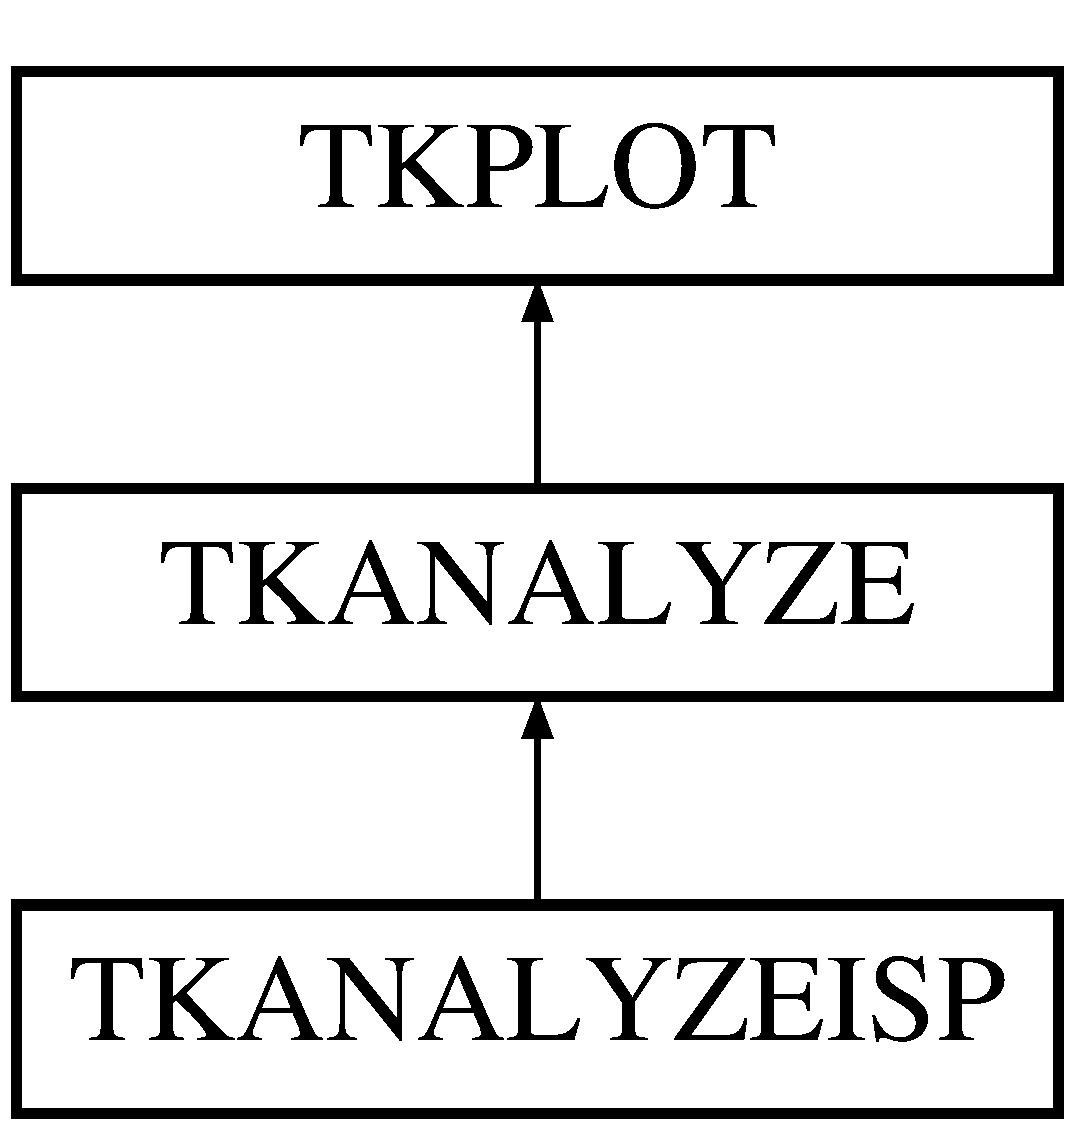
\includegraphics[height=3.000000cm]{class_t_k_a_n_a_l_y_z_e_i_s_p}
\end{center}
\end{figure}
\subsection*{公開メンバ関数}
\begin{DoxyCompactItemize}
\item 
\mbox{\Hypertarget{class_t_k_a_n_a_l_y_z_e_i_s_p_ad7af6efda43ab5c62bbddd8a8b39f2ef}\label{class_t_k_a_n_a_l_y_z_e_i_s_p_ad7af6efda43ab5c62bbddd8a8b39f2ef}} 
{\bfseries T\+K\+A\+N\+A\+L\+Y\+Z\+E\+I\+SP} (\hyperlink{class_t_k_s_h_o_t}{T\+K\+S\+H\+OT} $\ast$T\+K\+Shot\+\_\+, clx\+::ini $\ast$Setting\+\_\+, std\+::string group\+\_\+)
\item 
\mbox{\Hypertarget{class_t_k_a_n_a_l_y_z_e_i_s_p_a04ffee51cd9091aa6edb0ada63a0c455}\label{class_t_k_a_n_a_l_y_z_e_i_s_p_a04ffee51cd9091aa6edb0ada63a0c455}} 
int {\bfseries Plot\+Analyze\+SP} (\hyperlink{class_t_k_p_l_o_t_a158082ae168750554cf23edde9a27416}{T\+K\+P\+L\+O\+T\+::\+P\+L\+O\+T\+S\+I\+ZE} plot\+\_\+size, int shot\+\_\+number)
\end{DoxyCompactItemize}
\subsection*{その他の継承メンバ}


このクラス詳解は次のファイルから抽出されました\+:\begin{DoxyCompactItemize}
\item 
U\+I/\+Project1/tkanalyzeisp.\+h\end{DoxyCompactItemize}

\hypertarget{class_t_k_a_n_a_l_y_z_e_s_p}{}\section{T\+K\+A\+N\+A\+L\+Y\+Z\+E\+SP クラス}
\label{class_t_k_a_n_a_l_y_z_e_s_p}\index{T\+K\+A\+N\+A\+L\+Y\+Z\+E\+SP@{T\+K\+A\+N\+A\+L\+Y\+Z\+E\+SP}}
\subsection*{公開メンバ関数}
\begin{DoxyCompactItemize}
\item 
\mbox{\Hypertarget{class_t_k_a_n_a_l_y_z_e_s_p_aa2f68f6edb8adf34b6076f6826d56da8}\label{class_t_k_a_n_a_l_y_z_e_s_p_aa2f68f6edb8adf34b6076f6826d56da8}} 
{\bfseries T\+K\+A\+N\+A\+L\+Y\+Z\+E\+SP} (\hyperlink{class_t_k_s_h_o_t}{T\+K\+S\+H\+OT} $\ast$T\+K\+Shot\+\_\+, clx\+::ini $\ast$Setting\+\_\+)
\item 
\mbox{\Hypertarget{class_t_k_a_n_a_l_y_z_e_s_p_a1ba818f18587dca67f006dddcf38c774}\label{class_t_k_a_n_a_l_y_z_e_s_p_a1ba818f18587dca67f006dddcf38c774}} 
int {\bfseries Plot\+Raw} (T\+K\+P\+L\+O\+T\+::\+P\+L\+O\+T\+S\+I\+ZE plot\+\_\+size, int shot\+\_\+number)
\item 
\mbox{\Hypertarget{class_t_k_a_n_a_l_y_z_e_s_p_a287e554a4aee42c9232fe0d8b37f4fcb}\label{class_t_k_a_n_a_l_y_z_e_s_p_a287e554a4aee42c9232fe0d8b37f4fcb}} 
std\+::vector$<$ \hyperlink{struct_t_k_p_l_o_t_1_1_p_l_o_t_i_n_f_o}{T\+K\+P\+L\+O\+T\+::\+P\+L\+O\+T\+I\+N\+FO} $>$ {\bfseries Get\+Plot\+Info} ()
\item 
\mbox{\Hypertarget{class_t_k_a_n_a_l_y_z_e_s_p_ade64a95057a2325f7d210ee554ff5779}\label{class_t_k_a_n_a_l_y_z_e_s_p_ade64a95057a2325f7d210ee554ff5779}} 
std\+::vector$<$ \hyperlink{struct_t_k_p_l_o_t_1_1_p_l_o_t_i_n_f_o}{T\+K\+P\+L\+O\+T\+::\+P\+L\+O\+T\+I\+N\+FO} $>$\+::pointer {\bfseries Get\+Plot\+Info\+Ptr} ()
\end{DoxyCompactItemize}


このクラス詳解は次のファイルから抽出されました\+:\begin{DoxyCompactItemize}
\item 
tkanalyzesp.\+h\end{DoxyCompactItemize}

\hypertarget{class_t_k_d_a_t_a}{}\section{T\+K\+D\+A\+TA クラス}
\label{class_t_k_d_a_t_a}\index{T\+K\+D\+A\+TA@{T\+K\+D\+A\+TA}}
\subsection*{公開型}
\begin{DoxyCompactItemize}
\item 
\mbox{\Hypertarget{class_t_k_d_a_t_a_ab55f2c2d1c76bbeb3c1820ad2e749f38}\label{class_t_k_d_a_t_a_ab55f2c2d1c76bbeb3c1820ad2e749f38}} 
enum {\bfseries B\+Y\+T\+E\+O\+R\+D\+ER} \{ {\bfseries B\+I\+G\+\_\+\+E\+N\+D\+I\+AN}, 
{\bfseries L\+I\+T\+T\+L\+E\+\_\+\+E\+N\+D\+I\+AN}
 \}
\item 
\mbox{\Hypertarget{class_t_k_d_a_t_a_add3f58dbf65c97f4c9998e3a8b3f79fd}\label{class_t_k_d_a_t_a_add3f58dbf65c97f4c9998e3a8b3f79fd}} 
enum {\bfseries D\+A\+T\+A\+F\+O\+R\+M\+AT} \{ {\bfseries T\+R\+A\+CE}, 
{\bfseries B\+L\+O\+CK}
 \}
\end{DoxyCompactItemize}
\subsection*{公開メンバ関数}
\begin{DoxyCompactItemize}
\item 
\mbox{\Hypertarget{class_t_k_d_a_t_a_ad142911ef868b94bd2607ab4ca69f84d}\label{class_t_k_d_a_t_a_ad142911ef868b94bd2607ab4ca69f84d}} 
int {\bfseries Parse\+H\+DR} ()
\item 
\mbox{\Hypertarget{class_t_k_d_a_t_a_a64f288a761012bf276a5aa7f74dfcb44}\label{class_t_k_d_a_t_a_a64f288a761012bf276a5aa7f74dfcb44}} 
int {\bfseries Set\+A\+D\+C\+ID} (int iadc\+\_\+id)
\item 
\mbox{\Hypertarget{class_t_k_d_a_t_a_ad0a8defdf8de2ef2bbe42d7d8a53e051}\label{class_t_k_d_a_t_a_ad0a8defdf8de2ef2bbe42d7d8a53e051}} 
int {\bfseries Get\+A\+D\+C\+ID} ()
\item 
\mbox{\Hypertarget{class_t_k_d_a_t_a_ae63b673fda97ff6fef659f51fe40dbe8}\label{class_t_k_d_a_t_a_ae63b673fda97ff6fef659f51fe40dbe8}} 
int {\bfseries Set\+Data\+File\+Name} (std\+::string idata\+\_\+file\+\_\+name)
\item 
\mbox{\Hypertarget{class_t_k_d_a_t_a_a3f354a0eb29025867cbd1e3e27f8e41a}\label{class_t_k_d_a_t_a_a3f354a0eb29025867cbd1e3e27f8e41a}} 
std\+::string {\bfseries Get\+Data\+File\+Name} ()
\item 
\mbox{\Hypertarget{class_t_k_d_a_t_a_a0f0c38948586490c1bfe1f820418c5ef}\label{class_t_k_d_a_t_a_a0f0c38948586490c1bfe1f820418c5ef}} 
float {\bfseries Get\+H\+Resolution} ()
\item 
\mbox{\Hypertarget{class_t_k_d_a_t_a_a6c83babefbef168db08ca1c00cfe560d}\label{class_t_k_d_a_t_a_a6c83babefbef168db08ca1c00cfe560d}} 
float {\bfseries Get\+V\+Offset} (int const trace\+\_\+index)
\item 
\mbox{\Hypertarget{class_t_k_d_a_t_a_a78fccdabf4c7326ecb9dbe30ebe765e4}\label{class_t_k_d_a_t_a_a78fccdabf4c7326ecb9dbe30ebe765e4}} 
float {\bfseries Get\+V\+Resolution} (int const trace\+\_\+index)
\item 
\mbox{\Hypertarget{class_t_k_d_a_t_a_aaa91499a0c86542c6d240f07b2c7a5a6}\label{class_t_k_d_a_t_a_aaa91499a0c86542c6d240f07b2c7a5a6}} 
int {\bfseries Get\+V\+Max\+Data} (int const trace\+\_\+index)
\item 
\mbox{\Hypertarget{class_t_k_d_a_t_a_aed38093c0f7a086ab190c89770567531}\label{class_t_k_d_a_t_a_aed38093c0f7a086ab190c89770567531}} 
int {\bfseries Get\+V\+Min\+Data} (int const trace\+\_\+index)
\item 
\mbox{\Hypertarget{class_t_k_d_a_t_a_a5fe237cba051e352845786e13c0cd54f}\label{class_t_k_d_a_t_a_a5fe237cba051e352845786e13c0cd54f}} 
int {\bfseries Get\+Block\+Size} ()
\item 
\mbox{\Hypertarget{class_t_k_d_a_t_a_ac823854fcfb02d7788ec491b38f4d615}\label{class_t_k_d_a_t_a_ac823854fcfb02d7788ec491b38f4d615}} 
float {\bfseries Get\+H\+Offset} ()
\item 
\mbox{\Hypertarget{class_t_k_d_a_t_a_af0a676448ec4d492290517a7e60a2de3}\label{class_t_k_d_a_t_a_af0a676448ec4d492290517a7e60a2de3}} 
std\+::string {\bfseries Get\+Model\+Name} ()
\item 
\mbox{\Hypertarget{class_t_k_d_a_t_a_a63437cd1b2448b0b54ee6ec56da1321e}\label{class_t_k_d_a_t_a_a63437cd1b2448b0b54ee6ec56da1321e}} 
T\+K\+D\+A\+T\+A\+::\+B\+Y\+T\+E\+O\+R\+D\+ER {\bfseries Get\+Byte\+Order} ()
\item 
\mbox{\Hypertarget{class_t_k_d_a_t_a_a86117b4edecbf2e3013973fb016877e2}\label{class_t_k_d_a_t_a_a86117b4edecbf2e3013973fb016877e2}} 
T\+K\+D\+A\+T\+A\+::\+D\+A\+T\+A\+F\+O\+R\+M\+AT {\bfseries Get\+Data\+Format} ()
\item 
\mbox{\Hypertarget{class_t_k_d_a_t_a_a11fad512e15a5b8dd7be2ff786d5fd8e}\label{class_t_k_d_a_t_a_a11fad512e15a5b8dd7be2ff786d5fd8e}} 
int {\bfseries Get\+Data\+Offset} ()
\item 
\mbox{\Hypertarget{class_t_k_d_a_t_a_a0e9270376ed47917048fdd38f2f4a81d}\label{class_t_k_d_a_t_a_a0e9270376ed47917048fdd38f2f4a81d}} 
int {\bfseries Get\+Trace\+Total\+Number} ()
\item 
\mbox{\Hypertarget{class_t_k_d_a_t_a_ad70108b9612759566d7cc90e60f293c5}\label{class_t_k_d_a_t_a_ad70108b9612759566d7cc90e60f293c5}} 
int {\bfseries Channnel\+Number\+To\+Trace\+Number} (int const channel\+\_\+number)
\item 
\mbox{\Hypertarget{class_t_k_d_a_t_a_a8282e57fcee3618dfe533b6771adce96}\label{class_t_k_d_a_t_a_a8282e57fcee3618dfe533b6771adce96}} 
int {\bfseries Get\+Channel\+Number} (int const trace\+\_\+index)
\end{DoxyCompactItemize}


このクラス詳解は次のファイルから抽出されました\+:\begin{DoxyCompactItemize}
\item 
U\+I/\+Project1/tkshotinfo.\+h\item 
U\+I/\+Project1/tkshotinfo.\+cpp\end{DoxyCompactItemize}

\hypertarget{class_t_k_particle_palameter}{}\section{T\+K\+Particle\+Palameter クラス}
\label{class_t_k_particle_palameter}\index{T\+K\+Particle\+Palameter@{T\+K\+Particle\+Palameter}}
\subsection*{公開変数類}
\begin{DoxyCompactItemize}
\item 
\mbox{\Hypertarget{class_t_k_particle_palameter_a23ae16244a4143ee0642cf6620facf31}\label{class_t_k_particle_palameter_a23ae16244a4143ee0642cf6620facf31}} 
double {\bfseries density}
\item 
\mbox{\Hypertarget{class_t_k_particle_palameter_a65c396039f6aaf454837c2139af9da65}\label{class_t_k_particle_palameter_a65c396039f6aaf454837c2139af9da65}} 
double {\bfseries temperature}
\item 
\mbox{\Hypertarget{class_t_k_particle_palameter_a9be89d1ba1cb6c97e6154bf9f91f2437}\label{class_t_k_particle_palameter_a9be89d1ba1cb6c97e6154bf9f91f2437}} 
double {\bfseries mass}
\end{DoxyCompactItemize}


このクラス詳解は次のファイルから抽出されました\+:\begin{DoxyCompactItemize}
\item 
U\+I/\+Project1/tkphysics.\+h\end{DoxyCompactItemize}

\hypertarget{class_t_k_plasma}{}\section{T\+K\+Plasma クラス}
\label{class_t_k_plasma}\index{T\+K\+Plasma@{T\+K\+Plasma}}
\subsection*{公開変数類}
\begin{DoxyCompactItemize}
\item 
\mbox{\Hypertarget{class_t_k_plasma_ab2ba31fba9c3b255fa454d557b46c552}\label{class_t_k_plasma_ab2ba31fba9c3b255fa454d557b46c552}} 
double const  \& {\bfseries n\+\_\+e} = electron.\+density
\item 
\mbox{\Hypertarget{class_t_k_plasma_af742f3b64a9c48f6f0e3184bf7ebb0c2}\label{class_t_k_plasma_af742f3b64a9c48f6f0e3184bf7ebb0c2}} 
double const  \& {\bfseries n\+\_\+n} = neutral.\+density
\item 
\mbox{\Hypertarget{class_t_k_plasma_a0074fb0c178f69de84d5509d0bfd4ac0}\label{class_t_k_plasma_a0074fb0c178f69de84d5509d0bfd4ac0}} 
double const {\bfseries a}
\end{DoxyCompactItemize}


このクラス詳解は次のファイルから抽出されました\+:\begin{DoxyCompactItemize}
\item 
tkphysics.\+h\end{DoxyCompactItemize}

\hypertarget{class_t_k_plasma_parameter}{}\section{T\+K\+Plasma\+Parameter クラス}
\label{class_t_k_plasma_parameter}\index{T\+K\+Plasma\+Parameter@{T\+K\+Plasma\+Parameter}}


このクラス詳解は次のファイルから抽出されました\+:\begin{DoxyCompactItemize}
\item 
U\+I/\+Project1/tkphysics.\+h\end{DoxyCompactItemize}

\hypertarget{class_t_k_p_l_o_t}{}\section{T\+K\+P\+L\+OT クラス}
\label{class_t_k_p_l_o_t}\index{T\+K\+P\+L\+OT@{T\+K\+P\+L\+OT}}


{\ttfamily \#include $<$tkplot.\+h$>$}

T\+K\+P\+L\+OT の継承関係図\begin{figure}[H]
\begin{center}
\leavevmode
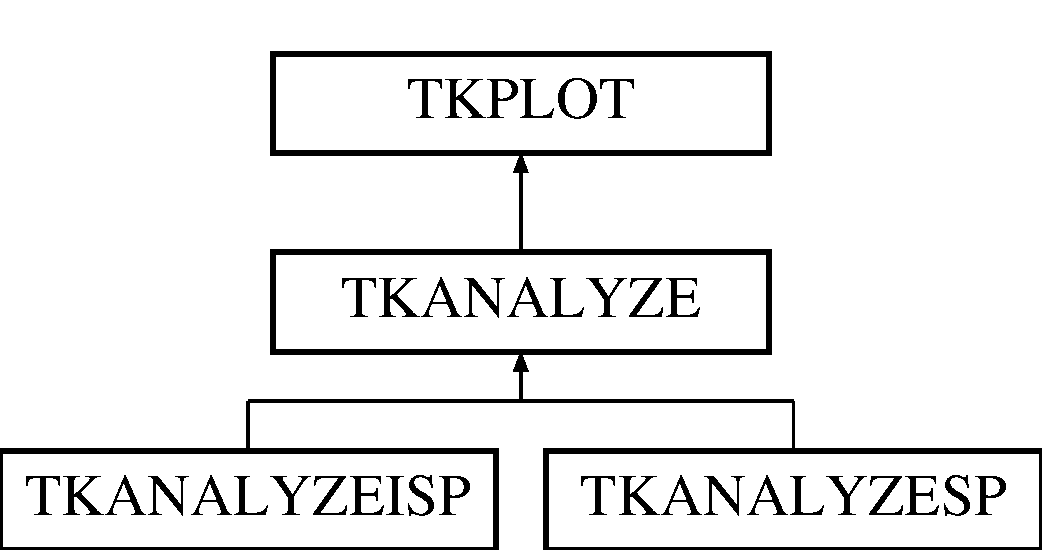
\includegraphics[height=3.000000cm]{class_t_k_p_l_o_t}
\end{center}
\end{figure}
\subsection*{クラス}
\begin{DoxyCompactItemize}
\item 
class \hyperlink{class_t_k_p_l_o_t_1_1_p_l_o_t_i_n_f_o}{P\+L\+O\+T\+I\+N\+FO}
\item 
class \hyperlink{class_t_k_p_l_o_t_1_1_p_o_s_i_t_i_o_n}{P\+O\+S\+I\+T\+I\+ON}
\item 
class \hyperlink{class_t_k_p_l_o_t_1_1_r_a_n_g_e}{R\+A\+N\+GE}
\item 
class \hyperlink{class_t_k_p_l_o_t_1_1_s_i_z_e}{S\+I\+ZE}
\end{DoxyCompactItemize}
\subsection*{公開型}
\begin{DoxyCompactItemize}
\item 
enum \hyperlink{class_t_k_p_l_o_t_a158082ae168750554cf23edde9a27416}{P\+L\+O\+T\+S\+I\+ZE} \{ {\bfseries S\+M\+A\+L\+L\+\_\+\+S\+I\+ZE}, 
{\bfseries M\+E\+D\+I\+U\+M\+\_\+\+S\+I\+ZE}
 \}
\item 
enum \hyperlink{class_t_k_p_l_o_t_a28dfea1dd78dfc49c1926518da615bfa}{D\+A\+T\+A\+S\+O\+U\+R\+CE} \{ \hyperlink{class_t_k_p_l_o_t_a28dfea1dd78dfc49c1926518da615bfaa98ad0e8750ae10ad556ed7a62affb452}{D\+A\+T\+A\+S\+O\+U\+R\+C\+E\+::\+B\+I\+N\+A\+RY}, 
\hyperlink{class_t_k_p_l_o_t_a28dfea1dd78dfc49c1926518da615bfaad2cd8253361a9c732d21ca1d336599cc}{D\+A\+T\+A\+S\+O\+U\+R\+C\+E\+::\+A\+S\+C\+II}
 \}
\end{DoxyCompactItemize}
\subsection*{公開メンバ関数}
\begin{DoxyCompactItemize}
\item 
\mbox{\Hypertarget{class_t_k_p_l_o_t_aeb9168bcf7e45c45fc38dab63e6b90b3}\label{class_t_k_p_l_o_t_aeb9168bcf7e45c45fc38dab63e6b90b3}} 
{\bfseries T\+K\+P\+L\+OT} (\hyperlink{class_t_k_s_h_o_t}{T\+K\+S\+H\+OT} $\ast$T\+K\+Shot\+\_\+)
\item 
\mbox{\Hypertarget{class_t_k_p_l_o_t_a0dcffb0672762042e8dca5791b97e182}\label{class_t_k_p_l_o_t_a0dcffb0672762042e8dca5791b97e182}} 
int {\bfseries Plot\+Raw} (const \hyperlink{class_t_k_p_l_o_t_a158082ae168750554cf23edde9a27416}{T\+K\+P\+L\+O\+T\+::\+P\+L\+O\+T\+S\+I\+ZE} plot\+\_\+size, const int shot\+\_\+number, bool replot=true)
\item 
\mbox{\Hypertarget{class_t_k_p_l_o_t_a5ddc4ef2a68d8649cfb2aebf507121fd}\label{class_t_k_p_l_o_t_a5ddc4ef2a68d8649cfb2aebf507121fd}} 
std\+::vector$<$ \hyperlink{class_t_k_p_l_o_t_1_1_p_l_o_t_i_n_f_o}{T\+K\+P\+L\+O\+T\+::\+P\+L\+O\+T\+I\+N\+FO} $>$ {\bfseries Get\+Plot\+Info} ()
\item 
\mbox{\Hypertarget{class_t_k_p_l_o_t_a4087cc1a73e760ac8eb32cbdf78a4433}\label{class_t_k_p_l_o_t_a4087cc1a73e760ac8eb32cbdf78a4433}} 
std\+::vector$<$ \hyperlink{class_t_k_p_l_o_t_1_1_p_l_o_t_i_n_f_o}{T\+K\+P\+L\+O\+T\+::\+P\+L\+O\+T\+I\+N\+FO} $>$\+::pointer {\bfseries Get\+Plot\+Info\+Ptr} ()
\end{DoxyCompactItemize}
\subsection*{限定公開メンバ関数}
\begin{DoxyCompactItemize}
\item 
\mbox{\Hypertarget{class_t_k_p_l_o_t_aae92c92917093101c52d08d132aee75b}\label{class_t_k_p_l_o_t_aae92c92917093101c52d08d132aee75b}} 
\hyperlink{class_t_k_p_l_o_t_1_1_p_l_o_t_i_n_f_o}{P\+L\+O\+T\+I\+N\+FO} \& {\bfseries load\+Plot\+Info\+Instance} (const int data\+\_\+index, const int trace\+\_\+index, const \hyperlink{class_t_k_p_l_o_t_a158082ae168750554cf23edde9a27416}{P\+L\+O\+T\+S\+I\+ZE} plot\+\_\+size=P\+L\+O\+T\+S\+I\+Z\+E\+::\+S\+M\+A\+L\+L\+\_\+\+S\+I\+ZE)
\end{DoxyCompactItemize}


\subsection{詳解}
グラフ描画に関するクラスです。 

\subsection{列挙型メンバ詳解}
\mbox{\Hypertarget{class_t_k_p_l_o_t_a28dfea1dd78dfc49c1926518da615bfa}\label{class_t_k_p_l_o_t_a28dfea1dd78dfc49c1926518da615bfa}} 
\index{T\+K\+P\+L\+OT@{T\+K\+P\+L\+OT}!D\+A\+T\+A\+S\+O\+U\+R\+CE@{D\+A\+T\+A\+S\+O\+U\+R\+CE}}
\index{D\+A\+T\+A\+S\+O\+U\+R\+CE@{D\+A\+T\+A\+S\+O\+U\+R\+CE}!T\+K\+P\+L\+OT@{T\+K\+P\+L\+OT}}
\subsubsection{\texorpdfstring{D\+A\+T\+A\+S\+O\+U\+R\+CE}{DATASOURCE}}
{\footnotesize\ttfamily enum \hyperlink{class_t_k_p_l_o_t_a28dfea1dd78dfc49c1926518da615bfa}{T\+K\+P\+L\+O\+T\+::\+D\+A\+T\+A\+S\+O\+U\+R\+CE}\hspace{0.3cm}{\ttfamily [strong]}}

データファイル形式型 \begin{DoxyEnumFields}{列挙値}
\raisebox{\heightof{T}}[0pt][0pt]{\index{B\+I\+N\+A\+RY@{B\+I\+N\+A\+RY}!T\+K\+P\+L\+OT@{T\+K\+P\+L\+OT}}\index{T\+K\+P\+L\+OT@{T\+K\+P\+L\+OT}!B\+I\+N\+A\+RY@{B\+I\+N\+A\+RY}}}\mbox{\Hypertarget{class_t_k_p_l_o_t_a28dfea1dd78dfc49c1926518da615bfaa98ad0e8750ae10ad556ed7a62affb452}\label{class_t_k_p_l_o_t_a28dfea1dd78dfc49c1926518da615bfaa98ad0e8750ae10ad556ed7a62affb452}} 
B\+I\+N\+A\+RY&バイナリファイル~\newline
 非常に高速に処理できますが、柔軟性にかけるため使用できないことがあります。 \\
\hline

\raisebox{\heightof{T}}[0pt][0pt]{\index{A\+S\+C\+II@{A\+S\+C\+II}!T\+K\+P\+L\+OT@{T\+K\+P\+L\+OT}}\index{T\+K\+P\+L\+OT@{T\+K\+P\+L\+OT}!A\+S\+C\+II@{A\+S\+C\+II}}}\mbox{\Hypertarget{class_t_k_p_l_o_t_a28dfea1dd78dfc49c1926518da615bfaad2cd8253361a9c732d21ca1d336599cc}\label{class_t_k_p_l_o_t_a28dfea1dd78dfc49c1926518da615bfaad2cd8253361a9c732d21ca1d336599cc}} 
A\+S\+C\+II&A\+S\+C\+I\+Iファイル~\newline
 データ変換のイニシャルタイムが必要であり、データ読み込みもハイコストなため、処理は遅くなりますが、全ての機能を利用できます。 \\
\hline

\end{DoxyEnumFields}
\mbox{\Hypertarget{class_t_k_p_l_o_t_a158082ae168750554cf23edde9a27416}\label{class_t_k_p_l_o_t_a158082ae168750554cf23edde9a27416}} 
\index{T\+K\+P\+L\+OT@{T\+K\+P\+L\+OT}!P\+L\+O\+T\+S\+I\+ZE@{P\+L\+O\+T\+S\+I\+ZE}}
\index{P\+L\+O\+T\+S\+I\+ZE@{P\+L\+O\+T\+S\+I\+ZE}!T\+K\+P\+L\+OT@{T\+K\+P\+L\+OT}}
\subsubsection{\texorpdfstring{P\+L\+O\+T\+S\+I\+ZE}{PLOTSIZE}}
{\footnotesize\ttfamily enum \hyperlink{class_t_k_p_l_o_t_a158082ae168750554cf23edde9a27416}{T\+K\+P\+L\+O\+T\+::\+P\+L\+O\+T\+S\+I\+ZE}\hspace{0.3cm}{\ttfamily [strong]}}

グラフサイズ型 

このクラス詳解は次のファイルから抽出されました\+:\begin{DoxyCompactItemize}
\item 
tkplot.\+h\end{DoxyCompactItemize}

\hypertarget{class_t_k_s_h_o_t}{}\section{T\+K\+S\+H\+OT クラス}
\label{class_t_k_s_h_o_t}\index{T\+K\+S\+H\+OT@{T\+K\+S\+H\+OT}}
\subsection*{公開メンバ関数}
\begin{DoxyCompactItemize}
\item 
\mbox{\Hypertarget{class_t_k_s_h_o_t_af116d5e195d9853c78d3e4ddb00e2c57}\label{class_t_k_s_h_o_t_af116d5e195d9853c78d3e4ddb00e2c57}} 
int {\bfseries Get\+A\+D\+C\+Number} ()
\item 
\mbox{\Hypertarget{class_t_k_s_h_o_t_a1314067d1c3ec702c29866ad124048eb}\label{class_t_k_s_h_o_t_a1314067d1c3ec702c29866ad124048eb}} 
std\+::string {\bfseries Get\+Data\+File\+Name} (int adc\+\_\+id)
\item 
\mbox{\Hypertarget{class_t_k_s_h_o_t_a8f91dff3640a574152c6fb3c5e542f62}\label{class_t_k_s_h_o_t_a8f91dff3640a574152c6fb3c5e542f62}} 
int {\bfseries Name\+Shot\+Number} (int ishot\+\_\+number)
\item 
\mbox{\Hypertarget{class_t_k_s_h_o_t_a8edc2c710c0dd04d619ddb5f105c41fe}\label{class_t_k_s_h_o_t_a8edc2c710c0dd04d619ddb5f105c41fe}} 
int {\bfseries Clear} ()
\item 
\mbox{\Hypertarget{class_t_k_s_h_o_t_ae8f63779c8d19ad6afab9e02ba066487}\label{class_t_k_s_h_o_t_ae8f63779c8d19ad6afab9e02ba066487}} 
int {\bfseries Append\+Data\+File} (std\+::string data\+\_\+file\+\_\+name)
\item 
\mbox{\Hypertarget{class_t_k_s_h_o_t_a055079afd19a206d3f525b6c2cbd5d75}\label{class_t_k_s_h_o_t_a055079afd19a206d3f525b6c2cbd5d75}} 
float {\bfseries Get\+H\+Resolution} (int adc\+\_\+id)
\item 
\mbox{\Hypertarget{class_t_k_s_h_o_t_abc9d569e4f7136cd0b3f56b8e0e2e8cd}\label{class_t_k_s_h_o_t_abc9d569e4f7136cd0b3f56b8e0e2e8cd}} 
int {\bfseries Get\+Block\+Size} (int adc\+\_\+id)
\item 
\mbox{\Hypertarget{class_t_k_s_h_o_t_ab43a63e3fe0f6797ee97eed0091339ba}\label{class_t_k_s_h_o_t_ab43a63e3fe0f6797ee97eed0091339ba}} 
float {\bfseries Get\+V\+Offset} (int adc\+\_\+id, int trace\+\_\+index)
\item 
\mbox{\Hypertarget{class_t_k_s_h_o_t_aafff8aa391415312187f769a4678c82f}\label{class_t_k_s_h_o_t_aafff8aa391415312187f769a4678c82f}} 
float {\bfseries Get\+V\+Resolution} (int adc\+\_\+id, int trace\+\_\+index)
\item 
\mbox{\Hypertarget{class_t_k_s_h_o_t_aa69c94f494055fd98ff3982681d6795c}\label{class_t_k_s_h_o_t_aa69c94f494055fd98ff3982681d6795c}} 
int {\bfseries Get\+V\+Max\+Data} (int adc\+\_\+id, int trace\+\_\+index)
\item 
\mbox{\Hypertarget{class_t_k_s_h_o_t_ab02def889d5bf8c6103dbac2a5f89ab6}\label{class_t_k_s_h_o_t_ab02def889d5bf8c6103dbac2a5f89ab6}} 
int {\bfseries Get\+V\+Min\+Data} (int adc\+\_\+id, int trace\+\_\+index)
\item 
\mbox{\Hypertarget{class_t_k_s_h_o_t_ae9bd114c4904e0f20929988b4307587f}\label{class_t_k_s_h_o_t_ae9bd114c4904e0f20929988b4307587f}} 
float {\bfseries Get\+H\+Offset} (int adc\+\_\+id)
\item 
\mbox{\Hypertarget{class_t_k_s_h_o_t_adb4af221e08781c6f742ff681d134163}\label{class_t_k_s_h_o_t_adb4af221e08781c6f742ff681d134163}} 
std\+::string {\bfseries Get\+Model\+Name} (int adc\+\_\+id)
\item 
\mbox{\Hypertarget{class_t_k_s_h_o_t_acfcfbf59a93120c97de2eee6acec5104}\label{class_t_k_s_h_o_t_acfcfbf59a93120c97de2eee6acec5104}} 
T\+K\+D\+A\+T\+A\+::\+B\+Y\+T\+E\+O\+R\+D\+ER {\bfseries Get\+Byte\+Order} (int adc\+\_\+id)
\item 
\mbox{\Hypertarget{class_t_k_s_h_o_t_a30ef4f11ad37a0e1ab3002d6e7a335d6}\label{class_t_k_s_h_o_t_a30ef4f11ad37a0e1ab3002d6e7a335d6}} 
T\+K\+D\+A\+T\+A\+::\+D\+A\+T\+A\+F\+O\+R\+M\+AT {\bfseries Get\+Data\+Format} (int adc\+\_\+id)
\item 
\mbox{\Hypertarget{class_t_k_s_h_o_t_ace4770ac6dcdec71ce95823689a58380}\label{class_t_k_s_h_o_t_ace4770ac6dcdec71ce95823689a58380}} 
int {\bfseries Get\+Data\+Offset} (int adc\+\_\+id)
\item 
\mbox{\Hypertarget{class_t_k_s_h_o_t_a45a19a71b5d82762601acef738ad504d}\label{class_t_k_s_h_o_t_a45a19a71b5d82762601acef738ad504d}} 
int {\bfseries Get\+Trace\+Total\+Number} (int adc\+\_\+id)
\item 
\mbox{\Hypertarget{class_t_k_s_h_o_t_a370000c7133ee68afe584d7c74864411}\label{class_t_k_s_h_o_t_a370000c7133ee68afe584d7c74864411}} 
int {\bfseries A\+D\+C\+I\+D\+To\+A\+D\+C\+Data\+Index} (int adc\+\_\+id)
\item 
\mbox{\Hypertarget{class_t_k_s_h_o_t_a5402cb531f82fe70ba46a4f0d97dfedf}\label{class_t_k_s_h_o_t_a5402cb531f82fe70ba46a4f0d97dfedf}} 
int {\bfseries Get\+A\+D\+C\+ID} (int adc\+\_\+index)
\item 
\mbox{\Hypertarget{class_t_k_s_h_o_t_a71522d246c17a4643838a01bef2943ff}\label{class_t_k_s_h_o_t_a71522d246c17a4643838a01bef2943ff}} 
int {\bfseries Get\+Channel\+Number} (int adc\+\_\+id, int trace\+\_\+index)
\end{DoxyCompactItemize}


このクラス詳解は次のファイルから抽出されました\+:\begin{DoxyCompactItemize}
\item 
tkshotinfo.\+h\end{DoxyCompactItemize}

\chapter{ファイル詳解}
\hypertarget{tkadc_8h}{}\section{U\+I/\+Project1/tkadc.h ファイル}
\label{tkadc_8h}\index{U\+I/\+Project1/tkadc.\+h@{U\+I/\+Project1/tkadc.\+h}}


A\+D\+Cをコントロールするためのクラスを宣言しています。 A\+D\+Cの制御に関して、モデルに依存する部分はここに記述してください。  


{\ttfamily \#include $<$string$>$}\newline
{\ttfamily \#include $<$iostream$>$}\newline
{\ttfamily \#include \char`\"{}tmctl.\+h\char`\"{}}\newline
\subsection*{クラス}
\begin{DoxyCompactItemize}
\item 
class \hyperlink{class_t_k_a_d_c_c_o_n_t_r_o_l}{T\+K\+A\+D\+C\+C\+O\+N\+T\+R\+OL}
\item 
class \hyperlink{class_t_k_a_d_c_c_o_n_t_r_o_l___d_l750}{T\+K\+A\+D\+C\+C\+O\+N\+T\+R\+O\+L\+\_\+\+D\+L750}
\item 
class \hyperlink{class_t_k_a_d_c_c_o_n_t_r_o_l___d_l850}{T\+K\+A\+D\+C\+C\+O\+N\+T\+R\+O\+L\+\_\+\+D\+L850}
\end{DoxyCompactItemize}
\subsection*{マクロ定義}
\begin{DoxyCompactItemize}
\item 
\mbox{\Hypertarget{tkadc_8h_adc3098545276669ab4c4771eb395bbc2}\label{tkadc_8h_adc3098545276669ab4c4771eb395bbc2}} 
\#define {\bfseries T\+K\+A\+D\+C\+\_\+\+A\+D\+C\+\_\+\+M\+O\+D\+E\+L\+\_\+\+D\+L750}~T\+K\+A\+D\+C\+C\+O\+N\+T\+R\+O\+L\+::\+A\+D\+C\+M\+O\+D\+E\+L\+::\+D\+L750
\item 
\mbox{\Hypertarget{tkadc_8h_a97e18823dd95e64bea5292f9d23ea048}\label{tkadc_8h_a97e18823dd95e64bea5292f9d23ea048}} 
\#define {\bfseries T\+K\+A\+D\+C\+\_\+\+A\+D\+C\+\_\+\+M\+O\+D\+E\+L\+\_\+\+D\+L850}~T\+K\+A\+D\+C\+C\+O\+N\+T\+R\+O\+L\+::\+A\+D\+C\+M\+O\+D\+E\+L\+::\+D\+L850
\item 
\mbox{\Hypertarget{tkadc_8h_a881027a2354a0e19afa983c2dc4b3e11}\label{tkadc_8h_a881027a2354a0e19afa983c2dc4b3e11}} 
\#define {\bfseries T\+K\+A\+D\+C\+\_\+\+A\+D\+C\+\_\+\+C\+H\+A\+N\+N\+E\+L\+\_\+\+M\+AX}~18
\end{DoxyCompactItemize}


\subsection{詳解}
A\+D\+Cをコントロールするためのクラスを宣言しています。 A\+D\+Cの制御に関して、モデルに依存する部分はここに記述してください。 

\begin{DoxyAuthor}{著者}
Kobayashi Takahiko 
\end{DoxyAuthor}
\begin{DoxyDate}{日付}
2017 
\end{DoxyDate}

\hypertarget{tkfileutil_8h}{}\section{tkfileutil.\+h ファイル}
\label{tkfileutil_8h}\index{tkfileutil.\+h@{tkfileutil.\+h}}


便利な汎用関数等です。  


{\ttfamily \#include $<$iostream$>$}\newline
{\ttfamily \#include $<$string$>$}\newline
{\ttfamily \#include $<$sstream$>$}\newline
{\ttfamily \#include $<$iomanip$>$}\newline
{\ttfamily \#include $<$fstream$>$}\newline
{\ttfamily \#include $<$vector$>$}\newline
{\ttfamily \#include \char`\"{}clx/salgorithm.\+h\char`\"{}}\newline
{\ttfamily \#include \char`\"{}tkutil.\+h\char`\"{}}\newline
\subsection*{クラス}
\begin{DoxyCompactItemize}
\item 
class \hyperlink{class_t_k_f_i_l_e_u_t_i_l_1_1_s_h_o_t_f_i_l_e_n_a_m_e}{T\+K\+F\+I\+L\+E\+U\+T\+I\+L\+::\+S\+H\+O\+T\+F\+I\+L\+E\+N\+A\+ME}
\end{DoxyCompactItemize}
\subsection*{名前空間}
\begin{DoxyCompactItemize}
\item 
 \hyperlink{namespace_t_k_f_i_l_e_u_t_i_l}{T\+K\+F\+I\+L\+E\+U\+T\+IL}
\begin{DoxyCompactList}\small\item\em 便利な汎用関数等です。 \end{DoxyCompactList}\end{DoxyCompactItemize}
\subsection*{関数}
\begin{DoxyCompactItemize}
\item 
std\+::string \hyperlink{namespace_t_k_f_i_l_e_u_t_i_l_afb1f2be7ac9b585fc688a2c9a0e50094}{T\+K\+F\+I\+L\+E\+U\+T\+I\+L\+::\+Binary\+To\+C\+SV} (std\+::string file\+\_\+path, bool force\+\_\+over\+\_\+write=false)
\item 
std\+::string \hyperlink{namespace_t_k_f_i_l_e_u_t_i_l_a021f69b1dbf05a9501e30326b836c2a9}{T\+K\+F\+I\+L\+E\+U\+T\+I\+L\+::\+Extract\+W\+DF} (std\+::string file\+\_\+path, bool force\+\_\+over\+\_\+write=false)
\item 
std\+::vector$<$ std\+::string $>$ \hyperlink{namespace_t_k_f_i_l_e_u_t_i_l_a378ed1b7bfa3028b922a122f72f38b28}{T\+K\+F\+I\+L\+E\+U\+T\+I\+L\+::\+Get\+Same\+Shot\+File\+Name} (std\+::string file\+\_\+path)
\item 
std\+::string \hyperlink{namespace_t_k_f_i_l_e_u_t_i_l_ae7b4e47d9221322ea5dbaaaefd83b2b6}{T\+K\+F\+I\+L\+E\+U\+T\+I\+L\+::\+Remove\+Extension} (std\+::string file\+\_\+path)
\end{DoxyCompactItemize}


\subsection{詳解}
便利な汎用関数等です。 

\begin{DoxyAuthor}{著者}
Kobayashi Takahiko 
\end{DoxyAuthor}
\begin{DoxyDate}{日付}
2017.\+5.\+14 
\end{DoxyDate}

\hypertarget{tkutil_8h}{}\section{tkutil.\+h ファイル}
\label{tkutil_8h}\index{tkutil.\+h@{tkutil.\+h}}


便利な汎用関数等です。  


{\ttfamily \#include $<$iostream$>$}\newline
{\ttfamily \#include $<$string$>$}\newline
{\ttfamily \#include $<$sstream$>$}\newline
{\ttfamily \#include $<$iomanip$>$}\newline
{\ttfamily \#include $<$fstream$>$}\newline
\subsection*{名前空間}
\begin{DoxyCompactItemize}
\item 
 \hyperlink{namespace_t_k_u_t_i_l}{T\+K\+U\+T\+IL}
\begin{DoxyCompactList}\small\item\em 便利な汎用関数等です。 \end{DoxyCompactList}\item 
 \hyperlink{namespace_t_k_u_t_i_l_1_1_literals}{T\+K\+U\+T\+I\+L\+::\+Literals}
\end{DoxyCompactItemize}
\subsection*{関数}
\begin{DoxyCompactItemize}
\item 
std\+::string \hyperlink{namespace_t_k_u_t_i_l_a02b37f2f23e258b7a44b83e1ac5b81b7}{T\+K\+U\+T\+I\+L\+::\+Zero\+Fill} (int const number, int const length)
\item 
bool \hyperlink{namespace_t_k_u_t_i_l_ab26eef58ef280f33492f52cb4fbe6b5d}{T\+K\+U\+T\+I\+L\+::\+Is\+Exist\+File} (std\+::string const file\+\_\+name)
\end{DoxyCompactItemize}


\subsection{詳解}
便利な汎用関数等です。 

\begin{DoxyAuthor}{著者}
Kobayashi Takahiko 
\end{DoxyAuthor}
\begin{DoxyDate}{日付}
2017 
\end{DoxyDate}

%--- End generated contents ---

% Index
\backmatter
\newpage
\phantomsection
\clearemptydoublepage
\addcontentsline{toc}{chapter}{索引}
\printindex

\end{document}
